%%% The main file. It contains definitions of basic parameters and includes all other parts.

%% Settings for single-side (simplex) printing
% Margins: left 40mm, right 25mm, top and bottom 25mm
% (but beware, LaTeX adds 1in implicitly)
\documentclass[12pt,a4paper]{report}
\setlength\textwidth{145mm}
\setlength\textheight{247mm}
\setlength\oddsidemargin{15mm}
\setlength\evensidemargin{15mm}
\setlength\topmargin{0mm}
\setlength\headsep{0mm}
\setlength\headheight{0mm}
% \openright makes the following text appear on a right-hand page
\let\openright=\clearpage

%% Settings for two-sided (duplex) printing
% \documentclass[12pt,a4paper,twoside,openright]{report}
% \setlength\textwidth{145mm}
% \setlength\textheight{247mm}
% \setlength\oddsidemargin{14.2mm}
% \setlength\evensidemargin{0mm}
% \setlength\topmargin{0mm}
% \setlength\headsep{0mm}
% \setlength\headheight{0mm}
% \let\openright=\cleardoublepage

%% Generate PDF/A-2u
\usepackage[a-2u]{pdfx}


%% Character encoding: usually latin2, cp1250 or utf8:
\usepackage[utf8]{inputenc}

%% Prefer Latin Modern fonts
\usepackage{lmodern}

%% Further useful packages (included in most LaTeX distributions)
\usepackage{amsmath}        % extensions for typesetting of math
\usepackage{amsfonts}       % math fonts
\usepackage{amsthm}         % theorems, definitions, etc.
\usepackage{amssymb}        % symbols
\usepackage{bbding}         % various symbols (squares, asterisks, scissors, ...)
\usepackage{bm}             % boldface symbols (\bm)
\usepackage{graphicx}       % embedding of pictures
\usepackage{fancyvrb}       % improved verbatim environment
\usepackage{natbib}         % citation style AUTHOR (YEAR), or AUTHOR [NUMBER]
\usepackage[nottoc]{tocbibind} % makes sure that bibliography and the lists
			    % of figures/tables are included in the table
			    % of contents
\usepackage{dcolumn}        % improved alignment of table columns
\usepackage{booktabs}       % improved horizontal lines in tables
\usepackage{paralist}       % improved enumerate and itemize
\usepackage{xcolor}         % typesetting in color

\usepackage{nameref}        % reference by name
\usepackage{mathtools}      % enhances the appearance of documents containing a lot of mathematics

\usepackage{todonotes}      % extension to typeset comments

\usepackage{multicol}       % support for table multi column
\usepackage{multirow}       % support for table multi row

\usepackage{makecell}       % easier support for multi row

\usepackage{pgf}            % use pgf backend
\usepackage{svg}            % draw svg figures

\usepackage{algorithm} 
\usepackage{algpseudocode} 

%%% Basic information on the thesis
% Thesis title in English (exactly as in the formal assignment)
\def\ThesisTitle{Fairness in group recommender systems}

% Author of the thesis
\def\ThesisAuthor{Bc. Ladislav Maleček}

% Year when the thesis is submitted
\def\YearSubmitted{2022}

% Name of the department or institute, where the work was officially assigned
% (according to the Organizational Structure of MFF UK in English,
% or a full name of a department outside MFF)
\def\Department{Department of Software Engineering}

% Is it a department (katedra), or an institute (ústav)?
\def\DeptType{Department}

% Thesis supervisor: name, surname and titles
\def\Supervisor{Mgr. Ladislav Peška, Ph.D.}

% Supervisor's department (again according to Organizational structure of MFF)
\def\SupervisorsDepartment{Department of Software Engineering}

% Study programme and specialization
\def\StudyProgramme{Informatics}
\def\StudyBranch{Artificial Intelligence}

% An optional dedication: you can thank whomever you wish (your supervisor,
% consultant, a person who lent the software, etc.)
\def\Dedication{%
\textcolor{red}{Dedication.}
}

% Abstract (recommended length around 80-200 words; this is not a copy of your thesis assignment!)
\def\Abstract{%
\textcolor{red}{Abstract}.
}

% 3 to 5 keywords (recommended), each enclosed in curly braces
\def\Keywords{group recommender systems, fairness, synthetic datasets, preference aggregation}


%% The hyperref package for clickable links in PDF and also for storing
%% metadata to PDF (including the table of contents).
%% Most settings are pre-set by the pdfx package.
\hypersetup{unicode}
\hypersetup{breaklinks=true}

% Definitions of macros (see description inside)
%%% This file contains definitions of various useful macros and environments %%%
%%% Please add more macros here instead of cluttering other files with them. %%%

%%% Minor tweaks of style

% These macros employ a little dirty trick to convince LaTeX to typeset
% chapter headings sanely, without lots of empty space above them.
% Feel free to ignore.
\makeatletter
\def\@makechapterhead#1{
  {\parindent \z@ \raggedright \normalfont
   \Huge\bfseries \thechapter. #1
   \par\nobreak
   \vskip 20\p@
}}
\def\@makeschapterhead#1{
  {\parindent \z@ \raggedright \normalfont
   \Huge\bfseries #1
   \par\nobreak
   \vskip 20\p@
}}
\makeatother

% This macro defines a chapter, which is not numbered, but is included
% in the table of contents.
\def\chapwithtoc#1{
\chapter*{#1}
\addcontentsline{toc}{chapter}{#1}
}

% Draw black "slugs" whenever a line overflows, so that we can spot it easily.
% \overfullrule=1mm

%%% Macros for definitions, theorems, claims, examples, ... (requires amsthm package)

\theoremstyle{plain}
\newtheorem{thm}{Theorem}
\newtheorem{lemma}[thm]{Lemma}
\newtheorem{claim}[thm]{Claim}

\theoremstyle{plain}
\newtheorem{defn}{Definition}

\theoremstyle{remark}
\newtheorem*{cor}{Corollary}
\newtheorem*{rem}{Remark}
\newtheorem*{example}{Example}

%%% An environment for proofs

\newenvironment{myproof}{
  \par\medskip\noindent
  \textit{Proof}.
}{
\newline
\rightline{$\qedsymbol$}
}

%%% An environment for typesetting of program code and input/output
%%% of programs. (Requires the fancyvrb package -- fancy verbatim.)

\DefineVerbatimEnvironment{code}{Verbatim}{fontsize=\small, frame=single}

%%% The field of all real and natural numbers
\newcommand{\R}{\mathbb{R}}
\newcommand{\N}{\mathbb{N}}

%%% Transposition of a vector/matrix
\newcommand{\T}[1]{#1^\top}

%%% Various math goodies
\newcommand{\goto}{\rightarrow}
\newcommand{\gotop}{\stackrel{P}{\longrightarrow}}
\newcommand{\maon}[1]{o(n^{#1})}
\newcommand{\abs}[1]{\left\lvert{#1}\right\rvert}
\newcommand{\dint}{\int_0^\tau\!\!\int_0^\tau}
\newcommand{\isqr}[1]{\frac{1}{\sqrt{#1}}}

%%% Various table goodies
\newcommand{\pulrad}[1]{\raisebox{1.5ex}[0pt]{#1}}
\newcommand{\mc}[1]{\multicolumn{1}{c}{#1}}

% Title page and various mandatory informational pages
\begin{document}
%%% Title page of the thesis and other mandatory pages

%%% Title page of the thesis

\pagestyle{empty}
\hypersetup{pageanchor=false}
\begin{center}

\centerline{\mbox{
\includegraphics[width=166mm]{img/logo-en.pdf}}}

\vspace{-8mm}
\vfill

{\bf\Large MASTER THESIS}

\vfill

{\LARGE\ThesisAuthor}

\vspace{15mm}

{\LARGE\bfseries\ThesisTitle}

\vfill

\Department

\vfill


\begin{tabular}{rl}
Supervisor of the bachelor thesis: & \Supervisor \\   
\noalign{\vspace{2mm}}
Study programme: & \StudyProgramme\\
\noalign{\vspace{2mm}}
Specialization: & \StudyBranch\\
\end{tabular}

\vfill

% Zde doplňte rok
Prague \YearSubmitted

\end{center}

\newpage

%%% Here should be a bound sheet included -- a signed copy of the "master
%%% thesis assignment". This assignment is NOT a part of the electronic
%%% version of the thesis. DO NOT SCAN.

%%% A page with a solemn declaration to the master thesis

\openright
\hypersetup{pageanchor=true}
\pagestyle{plain}
\pagenumbering{roman}
\vglue 0pt plus 1fill

\noindent
I declare that I carried out this master thesis independently, and only with the cited
sources, literature and other professional sources. It has not been used to obtain another
or the same degree.

\medskip\noindent
I understand that my work relates to the rights and obligations under the Act No.~121/2000 Sb.,
the Copyright Act, as amended, in particular the fact that the Charles
University has the right to conclude a license agreement on the use of this
work as a school work pursuant to Section 60 subsection 1 of the Copyright~Act.

\vspace{10mm}

\hbox{\hbox to 0.5\hsize{%
In \hbox to 6em{\dotfill} date \hbox to 6em{\dotfill}
\hss}\hbox to 0.5\hsize{\dotfill\quad}}
\smallskip
\hbox{\hbox to 0.5\hsize{}\hbox to 0.5\hsize{\hfil Author's signature\hfil}}

\vspace{20mm}
\newpage

%%% Dedication

\openright

\noindent
\Dedication

\newpage

%%% Mandatory information page of the thesis

\openright

\vbox to 0.5\vsize{
\setlength\parindent{0mm}
\setlength\parskip{5mm}

Title:
\ThesisTitle

Author:
\ThesisAuthor

\DeptType:
\Department

Supervisor:
\Supervisor, \SupervisorsDepartment

Abstract:
\Abstract

Keywords:
\Keywords

\vss}

\newpage

\openright
\pagestyle{plain}
\pagenumbering{arabic}
\setcounter{page}{1}


%%% A page with automatically generated table of contents of the master thesis

\tableofcontents

%%% Each chapter is kept in a separate file
\chapter{Introduction}  \label{chap_introduction}

% \addcontentsline{toc}{chapter}{Introduction}





Most of us interact with many recommender systems daily. Even if seemingly indirectly. The proliferation of this technology is astounding. Almost every interaction with today's web is in some way personalized. From the search results, shopping, listening to music, reading news, to browsing social media, and many more. Recommender systems has become quite literally unavoidable.

We can view recommender systems from a very simple perspective - they are algorithms that recommend items to users. Where items and users can be many different things, items, for example, being movies, news articles, a more complex object, or even entire systems. And users being, real people or other entities that exhibit some sort of preference on which the algorithm can decide.

One of the variants of recommender systems is those where the recommendation result is shared among more users based on their shared (aggregated) preferences. This is a subset called group recommender systems. They are not as widely used as the non-group variants, because we mostly use the web, listen to music and read the news as individuals. At least from the perspective of those systems. However, for some of the domains, there are valid use cases. We often listen to music and watch movies in groups. Select a restaurant and other public services not just for us. And that's where the group recommenders come in handy.

With groups as the target of a recommendation comes new challenges, among many others, how to measure satisfaction and ensure fairness among the group members. We first need to have a reliable way how to evaluate the recommendations. It starts to become harder than just simply rating the results based on single feedback, now we have multiple users with possibly very different personal experiences. We want to be fair towards all individuals in the group. But the fairness property can be tricky to describe and evaluate due to the subjective nature of preference perception and distribution among the group members.

Classical recommendation systems have been studied for quite a long time, but the group variant and more soft-level (meaning evaluation with metrics other than the classical accuracy and precision) thinking about them is quite recent. With the rise of social dilemmas around recommender systems is the fairness-ensuring topic becoming more important than before. And with that, there is growing popularity towards recommender systems that are trained (and therefore evaluated) with these novel requirements in mind.



\section{Problem statement}
The current research on the topic of group recommender systems is lacking. There are no standardized data sets that would offer evaluation of the research without using various methods of data augmentation and artificial data creation.
And the definition of fairness is not unified. It can mean many different things and be evaluated with many different methods.

These two aforementioned problems go hand in hand with the very subjective nature of user preference.
\todo[inline]{Mozna merge obou kapitol dohromady?}

\section{Research objective}

We would like to study how fairness can be defined in the context of the recommender systems, how it can be measured and eventually used to improve recommendations in the group setting. And explore different variants of fairness such as long-term fairness and different distribution of fairness among group members. 

The primary goal of this thesis is to research and design a novel group recommender system algorithm that would keep fairness as its primary optimization objective. If we could adapt fairness preserving methods such as voting systems from other fields to group recommendation problem. And evaluating the new algorithm with already existing approaches in the domain of group recommender systems.

Additionally, we would like to research and contribute to data sets that could be used for the group setting. Expanding single user data sets with data augmentation that would generate synthetic groups' information and creating a web application in a movie domain that would serve as a platform for online evaluation of group recommender algorithms and provided us with real-user group recommendation data.

\section{Thesis structure}

We start with an introduction to recommender systems and specifically to group recommender systems in the chapter: \nameref{chap:recommender_systems}. Then we will continue with the definitions and evaluation methods for fairness in chapter \nameref{chap:fairness}. Next, we will introduce few algorithms that are used in the group recommender field in chapter \nameref{chap:related_work}.
\textcolor{red}{TODO: check out other works and decide what should be here. This can be nice from the reading perspective, but is it really necessary?}




%%%%%%%%%%%%%%%%%%%%%%%%%%%%%%%%
% RECOMMENDER SYSTEMS
%%%%%%%%%%%%%%%%%%%%%%%%%%%%%%%%
\chapter{Recommender systems} \label{chap:recommender_systems}
In this chapter, we briefly introduce what recommender systems are (hereinafter referred to as RS), then continue with a description of the group variant of recommender systems and introduce common approaches and methods they employ.


\section{Recommender systems}\label{sec:01_rec_sys}
%\subsection{Introduction}
Broadly speaking, recommender systems are algorithms that suggest items to users. From another perspective, they aim to predict how a user would rate (like) an unseen item. They are used in various settings, for instance, e-commerce, media consumption, social networks, expert systems, search engines, and many others.

At their core, as stated in \cite{wiki:Recommender_system} they are essentially an information filtering system that aims to select a subset of items by some filtration criteria. In this case, the criteria are the user's preference. RS become necessary when it comes to suppressing the explosive growth of information on the web and function as a defense system against overloading the user with the vast amount of data that is present in almost every system today.

They can be viewed as decision support systems that guide users in finding and identifying items based on their idea about the desired state. In this situation, the desired state is to find an item that they would like \cite{grouprecommendersystems_felfernig2018group}.
 
RS can provide both by filtering based on user preference and providing alternatives by utilizing similarity. In a way, finding a suitable item can be viewed as a collaboration between the user and the recommender system, with varying degrees of freedom, from passively accepting the RS recommendations to actively interacting by giving feedback and stating preferences.

\subsection{High-level examples}\label{subsec:01_rec_sys.high_level_examples}
Recommender systems are used in multiple ways. We now present high-level examples of where and how they are utilized the most.
\begin{itemize}
    \item \textbf{Personalized merchandising}, where the system offers items that other users bought together with the viewed item. Items that a user could like based on the user's previous orders or viewed items.
    
    \item \textbf{Personalized content}, for content consumption services such as video and audio libraries. User is offered personalized content based on their preference profile, such as movies or videos that are similar to other content they consumed, globally popular for a regional subset of the user base, and so on.
    
    \item \textbf{Personalized news feed and social media feed}, offering users exciting content to keep them engaged with the service. In recent years there has been a push toward more socially responsible RS design in this context due to the overwhelming power of social media. It is important to deal with problems such as polarization \cite{recommender_systems_fighting_polarization}, fairness and disagreement.
    
    \item \textbf{Expert systems}, helping doctors, operators, and other people to make informed decisions based on data. They can help to deal with data overload and filter relevant items and choices. As well as explore the item space when searching for solutions with only weakly defined requirements.
    
    \item \textbf{Search experience}, that considers previous searches, preference profile, location, and other attributes.
\end{itemize}


\subsection{Main algorithmic approaches}\label{subsec:01_rec_sys.main_alg_approaches}

We can generally divide them by their approach mentioned in \cite{RS_handbook-ricci2011} and \cite{constraint_based_recommenders} into:
\begin{itemize}
    \item \textbf{Collaborative filtering} (CF)\newline
        Solely based on feedback from users (user-item interactions). Trying to recommend unseen items liked by users with a similar taste based on other items they have both rated. And thus exploiting data of users with similar preferences.
    \item  \textbf{Content-based filtering} (CB)\newline
        Uses item features or descriptions to recommend items similar to those the user liked or interacted with. We are essentially building a model of preference for users and exploiting domain knowledge about items that match the users' model.
    \item \textbf{Constraint-based recommendation}\newline
        It depends on hand-crafted deep knowledge about items. The user specifies a set of criteria based on which the system filters out items that meet the stated requirements. Additionally, the system can sort the items based on their properties if the stated criteria come with perceived importance - utility.
    \item \textbf{Hybrid systems}\newline    
        Combining multiple RS, either of the same type (with different parameters) or different types. This technique aims to increase recommendation efficacy. Main types according to \cite{grouprecommendersystems_felfernig2018group} are:
        \begin{itemize}
            \item Weighted where predictions of individual recommenders are summed up.
            \item Mixed, where predictions of individual recommenders are combined into one list.
            \item Cascade, where predictions of one recommender are fed as an input to another.
        \end{itemize}
\end{itemize}

The popularity of the first two approaches varies from domain to domain. Some domains naturally contain item-specific data, which allows for the use of \textit{content-based filtering}, for example, product parameters in e-shops. However, other domains do not. Then it is more beneficial to use \textit{collaborative filtering} techniques or a mix of the two.

There are benefits and drawbacks to both. CF can extract latent meaning from the data that would remain inaccessible to CB that relies on items' features. However, at the same time, it can cause problems to rely only on user-item interactions because we need a large amount of data to make a precise recommendation. There will be nothing to recommend if we cannot find similar enough other users that already rated some unseen items. This problem is called a \textit{cold-start problem}.

The third technique, \textit{Constraint-based filtering}, requires a deep knowledge that describes items on a higher level and is not very interesting due to the algorithmic simplicity. We will thus not discuss it further.

One other approach we did not include in the list is \textit{Critique-based recommendation}. Its popularity is relatively low, but it is still worth mentioning. It acts as a guide through the item space, where in cycles, we show the user items that are distinct in some property (we could say they lie in different areas of the item space), and the user either accepts or rejects them. Based on this feedback(critique) from the user, we narrow down the user's preferences, offer different (filtered/extended) set/sets of items, and try to guide the user to a satisfactory result. The feedback can, in some cases be provided for not just the item but even specifically for its properties or part of the items. An example could be: 'This carpet has a beautiful pattern, but the color is not that nice'.

%\todo[inline]{Jeste k tem critiquing, v nekterych pripadech API melo umoznit uzivateli rict, ktera vlastnost/oblast objektu nevyhovuje a tomu prizpusobit dalsi doporuceni - muzes zminit...}

Some of the classical and more advanced methods include:
\begin{itemize}
    \item User-based and item-based nearest neighbor similarity \cite{hill1995recommending}\cite{shardanand1995social}\cite{balabanovic1997fab}
    \item Matrix Factorisation techniques\cite{koren2009matrix}
    \item Deep Collaborative filtering \cite{he2017neural}\cite{YOUTUBE_deeprec-covington2016}\cite{DeepLearningBasedRecommenderSystem_zhang2019deep}
    \item Deep Content extraction\cite{DeepLearningBasedRecommenderSystem_zhang2019deep}
\end{itemize}



%%%%%%%%%%%%%%%%%%%%%%%%%%%%%%%%
% GROUP RECOMMENDER SYSTEMS
%%%%%%%%%%%%%%%%%%%%%%%%%%%%%%%%

\section{Group recommender systems} \label{sec:01_group_rec_sys}

So far, we have discussed only recommender systems, where an object of a recommendation is a single user (from now on referred to as single-user RS or simply as RS, depending on the context). However, what do we do when we have a group of users we want to recommend to? For example, a group of friends selecting a movie they want to watch or a group of colleagues listening to music together?  %We use a group recommender system (group RS). Where the objective of the system is to

Group recommender systems (group RS or GRS) are an interesting subarea of recommender systems, where the object of a recommendation is not just a single user but multiple individuals forming a group. The results of a recommendation for the group do need to reflect and balance individual preferences among all members.


\subsection{Characteristics of group RS}

There are many specifics that contrast GRS with single-user RS. Usually, some form of aggregation needs to be performed to transition from a single user preference that we gather to a recommendation for an entire group.

Situations differ for small and big groups, where the complexity of the users' preferences increases with the increasing number of users. At the same time, every person is different, some may be more forgiving, and some may be less willing to conform to a different set of tastes than their own.

Although there are not many reported deployments of such systems yet, we see domains that would greatly benefit from using GRS.

Two domains, in particular, come to mind: movie recommendation and music recommendation. In recent years with the rise of popularity of streaming services such as Netflix and Spotify, there finally exists enough data and, more importantly, a proliferation of these services that would allow the utilization of GRS.

Group recommendation systems usually operate on top of single-user RS and then perform some aggregation in order to provide the user group with relevant recommendations. There are two main types of GRS. The first aggregates user preferences that are fed to a single-user recommender system. The second performs the aggregation on the output of a single-user RS and, in some way, aggregates the recommended items of each group member into a single list. We will talk in-depth about the possible methods and strategies in Chapter \ref{chap:related_work}.

In our work, we focus on the second type that performs aggregation on top of an output of a single-user RS.


\subsection{Challenges}\label{subsec:01_group_rec_sys.challenges}

We now mention some of the most critical challenges in the group recommendation domain.

\begin{itemize}
    \item \textbf{How to merge individual preferences} \newline
        The main problem when extending RS systems to support the group setting is how to combine individual users' preferences. It is possible not to support groups at all and let users deal with the act of combining them via discussion. However, the problem then collapses back to a single-user setting, where the user represents the whole group. Therefore, we need to decide how and when to merge them. The main two approaches are mentioned in Subsection \ref{subsec:01_group_rec_sys.common_aproaches}.
        
    \item \textbf{Divergent group preferences} \newline
        Some users are so-called \textit{Grey-sheep} and \textit{Black-sheep}. These users are hard to recommend to because their preferences do not align with many or any other users (respectively). This problem is especially hard to solve in Collaborative filtering, which directly relies on finding similarities between users. Furthermore, the same problem arises in the group setting, where it becomes much harder to find solutions that would be satisfactory to all of its members. So in Group RS, the problem of outlying users can be observed on two levels, in the usual situation, where the group aggregated preferences are outlined, and on another level, where the inter-group preferences of individual users do not match.
    \item \textbf{Feedback gathering} \newline
        In most applications, feedback is gathered explicitly as well as implicitly. Explicitly by users rating recommended items and implicitly by the system observing users' behavior, such as which items they have visited or how long they have interacted with the item. Gathering direct feedback in the group setting is still possible, even if it is more problematic due to the possibility that not all members leave a rating. In some cases, gathering indirect (implicit feedback) can become even impossible, depending on how the system-user interactions are designed. In most cases, users will be selecting an item on a single device under one person's account. Therefore, it is hard to distinguish between the preferences of that one individual and the preferences of the group.
    \item \textbf{Active/passive, primary/secondary group members} \newline
        Another interesting issue arises when we consider that possibly not all members are equally important in the recommendation, as mentioned in \cite{deCampos_2009_managing_uncertanity_in_grouprec}. One example could be when parents select a movie to watch with their children. The children should (arguably) be given priority over the selection. A second example could be that we would want to prioritize the satisfaction of individuals in the group who were less satisfied the last time an item was consumed.
        
    \item \textbf{How to explain provided recommendations} \newline
    Explanation of single-user RS is already pretty challenging. With algorithms such as collaborative filtering, it is hard to explain why we are recommending an item apart from the obvious explanation that similar users liked this item. And with more advanced methods based on neural networks or more latent modeling of similarity and preference in general, it gets even more complex.
    
    This situation gets even worse, and another level of complexity emerges when we add the aggregation step to the recommendation process. 
    
    \item \textbf{Not all members present} \newline
    What can be done if we have a GRS preference model/data for a specific group and some of the members of that group are missing? We need to be able to modulate what members will be part of the recommendation process. This makes gathering and using feedback that would represent the whole group difficult.
    
    Another problem not entirely relevant to our work but still important is how we even know which group members are present. Many solutions exist, but they are not as seamless as the single-user variant, which is maybe one of the reasons why we do not see any widespread utilization of GRS so far.
    
    \item \textbf{Selecting from the provided list} \newline
    Providing the group with recommendations is an algorithmic task, but we need to take the presentation and how the users operate the service into account too. If, for example, one specific group member is selecting an item for the whole group, let's say, a movie to watch, this member will most probably have the easiest way to propagate their feedback to the selection. Therefore we need to take the implicit feedback with a grain of salt and not consider it as an implicit feedback from the whole group.
    
    Further, graphical user interfaces and the setup of the whole service, how users interact and select items, leave feedback, and other factors become important.
    
\end{itemize}


\subsection{Classification}
We now mention some basic classifications found in \cite{masthoff_2011_group_rec_systems}.
\begin{itemize}
    \item \textbf{Individual preferences are known vs. developed over time}
    
    Some GRS start with a good knowledge of the preference of each group member, such as if we have a system on a popular music streaming service. On the other hand, some systems, such as expert recommender systems, can even start with no information about the group members. It then needs to develop and model these preferences over time using a critique approach.
    
    \item \textbf{Real time consumption vs. option presentation}

    There are two options for GRS recommendation depending on how the items are consumed.
    
    Firstly, we can provide a set of items that are further filtered by the group members before they select an item that they like. In this case, when the list is further narrowed down by the group members, we can recommend more controversial item options.
    
    Secondly, when the recommendations are immediately consumed, such as a music playlist at a social event. We miss the selection process with which the group members narrow down the items list. In this case, one good option is to present the users with a list of already liked/seen items. This playlist would be composed of items the users like on their own.
    
    
    
    \item \textbf{Group preference weight is identical vs. alterable}
    
    There are situations in which the priority of group members differs when it comes to satisfaction. We can have systems that allow setting different weights for individual members.
    
    \item \textbf{Type of recommendation output}
    
    We can have many types of outputs from the recommender system. Such as a single item, a list of a predefined length, a set that does not have an explicit order, and others. The output in the case of expert systems can be a graph, a set of rules, or a feedback-gathering question.
    
    \item \textbf{Single vs. k-item utility}
    
    Another difference is how are the resulting recommended items processed by the users as presented in \cite{xiao_2017_fairness_aware_g_rec},\cite{connor_2001_polylens_rec_for_groups}. Do they select a single item, as is the case when recommending a list of movies? Do they consume the full list, such as playlist generation in the music domain? We must gather feedback and calculate the possible utility separately in these cases.
\end{itemize}


\subsection{Common approaches}\label{subsec:01_group_rec_sys.common_aproaches}

% \todo[inline]{Mention ephemeral vs persistent from paper PolyLens: A Recommender System for Groups of Users}
Now we introduce the two main algorithmic approaches of group recommender systems, according to \cite{recommendations_to_groups-jameson2007} these are:
\begin{itemize}
    \item \textbf{Group aware RS approach}\newline
    Builds a model for the group based on all its members' preferences. Either directly by creating a model of preference for the group or by aggregating models of individual users together and then recommending items for the group as a single entity.
    \item \textbf{RS aggregation approach}\newline
    Use single-user RS to recommend to each individual in the group and then aggregate the results together to create the final recommendation for the group.
    
    We can further split the aggregation approaches by where the aggregation takes place into the following two groups.
    
    \begin{itemize}
        \item Aggregation of individuals' preferences before the recommendation and then performing recommendation as if the preference belonged to a single user.
        \item Aggregation on top of recommendation results for individual users.
    \end{itemize}
    
    We will further mention these two approaches in detail in Subsection \ref{subsec:03_simple_aggregation_methods.methods}.
    
    % Firstly, aggregation of individuals' preferences before the recommendation and then performing recommendation as if the preference belonged to a single user.
    
    % Secondly, aggregation on top of recommendation results for individual users. We will further mention these two approaches in detail in \ref{subsec:03_simple_aggregation_methods.methods}.
    
\end{itemize}

% \todo[inline]{Mention division into groups based on where the recommender is "located" in relation to the aggregation, in short and then ref. the reader to the related work chapter where we discuss in depth. Or move the division from the related work here?}

In the RS aggregation approach, we further distinguish between two situations. A situation where we have predictions for all possible items and, therefore, can aggregate directly on the ratings of all items. And a situation where we only have a list of items (a subset of all items) for each user. These two can function very differently, for example, taking in context only the position in the recommended list or position and the rating. They are mentioned separately in \cite{recommendations_to_groups-jameson2007}. From a different point of view, they only differ in the availability of provided results from the underlying RS, so we group them under one main direction.

Further, both group-aware RS and aggregation approaches have advantages and disadvantages. One of the advantages of the Aggregation approach is that we can use the same RS as we would use for an individual recommendation. Either as a black box, directly performing aggregation on the top items that the black box provided, or in a more involved way by utilizing the predicted ratings. However, the aggregation strategies do rely on single-user RS so there is not much that can be done in order to extract some hidden latent preferences of the group, which in the case of the first method, the group-aware approach, can potentially be extracted.


We will discuss techniques from the latest literature in-depth in Chapter \ref{chap:related_work}.


At the same time, we need to define what it even means to recommend something to a group. Do we measure it by fairness, overall user satisfaction, or by the least satisfied member of the group? We will describe common approaches to these problems in Chapter \ref{chap:fairness}.
\chapter{Fairness} \label{chap:fairness}
% TODO: Introduction into the chapter, what we want to achieve, that we want try to define what Fairness is and how to measure it.

% TODO: Reword
So far, we have discussed recommender systems and the methods that are used in the field. But now, let us step back and look at the problem from a broader perspective of fairness as a social construct. Specifically, we will focus on the importance of fairness in the context of algorithms, what role it plays when using machine learning models with potentially sensitive data and see how and if we can make group recommenders better when we understand and define the underlying properties.

We will start with a general introduction to the topic of fairness, define its possible meanings and specify which one is important in our setting.
%\todo[inline]{vete chybi subject (we)}
This is required due to the overload of the word itself and the rising importance of the topic in today's world. Furthermore
%\todo[inline]{spis furthermore?}
, we will explain why fairness seems to be a crucial parameter in the group recommender setting and will try to reason about how to measure its effects.




\section{General} \label{sec:02_general}
% TODO: Start with a broad overview, why do we need something like fairness, define it, speak about it broadly.
% TODO: Problems with fairness, areas of usage, many possible definitions.

% I want to make an argument, that fairness is important to prevent notions of inequality which inherently leads to negative emotions

% it should lead the reader to think about it more, all the things we are discussing are general knowledge, we are not introducing something crazy

% IDEAS: Mention usage of the word fair/fairness
% https://www.youtube.com/watch?v=dKob6b8QzkU
% monkeys 
% https://www.youtube.com/watch?v=vHE6AYNOCrg
% many meaning of the word fairness, what does it mean for something to be fair

% the notion of fairness is probably important for developing cooperation

The word fairness
%\todo[inline]{pridal bych "fairness"}
itself is very hard and controversial to define.
%\todo[inline]{pridal bych carku}
In Cambridge Dictionary \cite{fairness_definition} it is
%\todo[inline]{zkracene is za 's se obecne nedoporucuje uvadet ve vedeckych textech - dobre pravidlo je ze apostroph je prijatelny jen u privlastnovacich vyrazu (John's shoe)}
defined as "The quality of treating people equally or in a way that is reasonable." Its use has been rising steadily from the 1960s as we can see on \ref{fig:popularity_of_fairness}.

\begin{figure}[htbp]
    \centering
    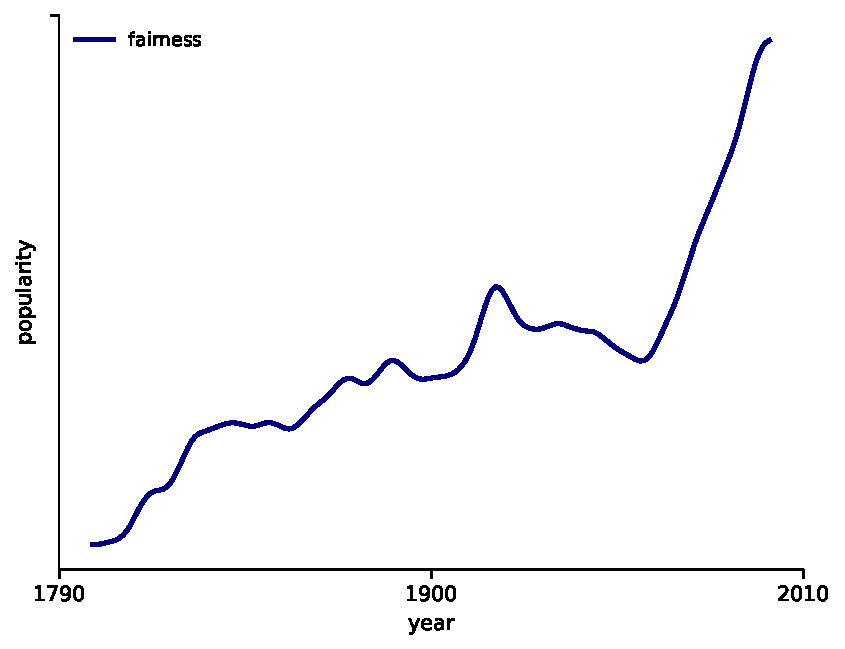
\includegraphics{img/google_ngram_fairness-eng_2012-1800-2000.pdf}
    \caption{The graph shows the phrase "fairness" occurring in the corpus of English books from 1800 to 2010. Source: Google Ngram Viewer, corpora 2012. \cite{google_ngram_viewer_2012}}
    \label{fig:popularity_of_fairness}
\end{figure}

Humans are obsessed with fairness. From a young age, children will get sad when something is not fair, when their sibling gets a more significant piece of a pie, more attention from their parent, or any other unequal situation. It can induce strong emotions such as envy, sadness, or anger, and it emerges very early, as early as 12 months of age or sooner as researched in \cite{children_fairness}.

And this behavior is not limited only to humans. We can observe the same behavior in monkeys. In \cite{brosnan2003monkeys}, the authors observed that if a monkey is getting the worse reward for the same task as its peer,  it refuses the reward and demands the same payout even if they were satisfied with the lesser reward for the same task before. In some sense, this is very strange, why should you care about someone having more if you have enough?

We observe the same behavior in many other species of animals, but not all. It seems that it requires a certain level of intelligence for the notion of fairness to emerge. As discussed in \cite{brosnan2014evolution}, based on studies of other non-human species, this evolutionary puzzle can be further dissected into responses to reward distribution among the cooperating group members. Where humans are willing to seek equalization of outcomes even if it means that they will loose some of their own reward as studied in \cite{willing_to_pay_to_equality}. At the same time, we humans like "free-rides" where we get high rewards for a small amount of work but dislike when someone else gets the same. This directly corresponds with the fairness itself - "It is not fair if someone else gets something we don't.". However, it all depends on our personality and the type of relationship involved. Some people are, for example, willing to accept that their partner makes more, but that is very subjective and in some cases can lead even to larger envy involved.

In some cases we observe a pattern of generosity, where children are willing to make their own sacrifices in order to ensure fairness, so that the other person does not have less than them, as presented in \cite{children_generocity_blake}. The authors studied fairness in multiple cultural settings and found out that this behavior is learned and only present in some cultures.

On the other hand, our society widely accepts the notion of "winner takes all", which can be problematic in itself, for example, in sports and business. In business it directly shapes the distribution of wealth, which is considered as one of the main problems of today's world. But discussing the social aspect of fairness is beyond the scope of this thesis.

When it comes to the true nature of fairness on the deepest level, it could even be possible that the notion of fairness emerges together with cooperation and therefore language and communication. It would mean that it is an inherent property of any intelligent agent that is created through an evolutionary process.
Another point of view could be that fairness acts as a mechanism that pushes towards equality among the group members and that leads to a higher stability of the group which would give an evolutionary advantage.
But more research has to be done, as our understanding of intelligence, consciousness, and related hard to quantify phenomena is lacking.\newline

Let us now get back to fairness in the context of computer systems.







\section{Algorithmic fairness}\label{subsec:02_general.algorithmic_fairness_and_possible_meanings}
% The Emerging Theory of Algorithmic Fairness
We will focus on fairness regarding society or individuals interacting with a computer system. We will not discuss further any meaning of fairness outside of the domain of computer science. This topic steers away from the main goal of defining fairness for the group RS sub-domain, but we think that it is very important topic in general, deserves more spotlight and can be a good middle step to understand specifics of the group RS setting.

\subsection{Sources of algorithmic unfairness}
%\todo[inline]{Pokud bys chtel neco formalnejsiho tak jako nadpis navrhuju Sources of algorithmic unfairness. Jinak ja bych tu variantu ze algoritmus je by design neferovy uplne nevyhazoval out of consideration. Treba cinsky credit score system - aneb je fer ze si nesmis koupit letenku protoze jsi prechazel na cervenou?}
%\todo[inline]{mozna radeji no understanding? Notion by mohl byt prosty fakt ze zna atribut}
%\todo[inline]{tahle veta je divna, chtelo by to lepe navazat - co  myslis tim ze autori algoritmu jsou lide - ze napsali ten alg. tak aby byl biased? Ze neco prehledli? Chtelo by to rozvest...}

How can a computer that has no underlying understanding of race or ethnicity discriminate against a group of people? At first this idea may seem strange, but we have to remember, that as with any other computer program, machine learning algorithms are designed by people. Data that is used to train those algorithms come from the real world, where bias and unfairness is unfortunately still present. And so, the trained models even if not usually meant with an ill-fated purpose will reflect that and in most cases include some form of bias or unfairness.
Of course, there exist uses of ML with bias that has been introduced on purpose. We can see that for example in the Chinese credit score system which is biased towards an individual based their class, race, political views and other factors which we, in the modern democratic world, consider as protected(sensitive) characteristics, which are not to be used as discrimination against an individual. But this type of bias in those circumstances is a knowingly designed and required feature of the system and therefore we will not discuss these systems any further.

In a more rigorous way, we can say that output of any machine learning (ML) algorithm is usually just a product of the underlying data. By design, accurate classifier will reproduce patterns found in the training data. And usually the bias is either transferred directly from the data or by wrongly defining the learning objective.

%At first, the idea of a machine being unfair may feel strange. How can a computer that has no understanding of race or ethnicity discriminate against a group of people? As with other computer programs, those who create the algorithms are people still people. Gathered data that are used to train the algorithm are from the real world. And so they reflect biases that are present in society. Algorithms with bias are not written with ill-fated purpose, it is usually just a side effect.
%\todo[inline]{Je to tak vzdy? pouzij neco jako "obvykle"}
%We can say that the results of any machine learning (ML) algorithm are just the product of the underlying data. By design, accurate classifier will reproduce patterns found in training data. 

%\todo[inline]{Celkove tenhle uvod by chtel jeste aspon jednou projit a idealne prepsat - mas tady hromadu myslenek ktere jsou sice asi validni, ale nejsou dobre provazane, nejsou rozvedene a ctenar z toho pak ma chaos.}


%Research of algorithm fairness tries to analyze machine learning algorithms and data gathering and processing with the goal of understanding how bias in them is created and how it can be fixed.
% \newline
Let us now present a division by the main sources of unfairness as stated in \cite{pessach2020algorithmic_fairness} with examples following in \ref{subsec:02_algo_fairness.examples_of_algo_biass}:
\begin{itemize}
    \item \textbf{Biases already included in the data set}\newline
    Such as dependence/correlation of data based on sensitive characteristics. Bias found in the data is by design reproduced by an accurate classifier.
    \item \textbf{Biases caused by missing data}\newline
    Missing or filtering out some of the training data can results in a data set that does not represent the target population.
    \item \textbf{Biases stemming from algorithmic objectives}\newline
    While training, we usually minimize some error, but that can lead to prioritization of interests of majority if left unchecked. It will always be easier to optimize results for groups with small entropy, than for niche groups that are more surprising and thus having a larger entropy.
    \item \textbf{Biases caused by "proxy" attributes}\newline
    Some attributes that are not directly considered sensitive still can contain information from sensitive attributes. In other words, they are not independent. The algorithm can therefore use the "proxy" attribute and exploit the sensitive attribute indirectly.
\end{itemize}

%\todo[inline]{Tenhle bullet list by snesl kazdy nejaky priklad kdy to nastane - ja sice vim o jake problemy se jedna, ale z toho popisu samotneho bych se toho IMO zas tak moc nedozvedel - kdyz tam uvedes vzdycky jeden konkretni priklad, bude to lepsi. Ted ctu ze mas priklady dal, tak mozna sem jen zminku o tom ze detailed examples later.}


It is important to define which sensitive characteristics need to be taken into account. As stated in \cite{european-union-agency-for-fundamental-rights-2018} those are: gender, ethnicity, sexual orientation, disability, and others. Most research in the domain of bias and fairness is, based on our perception, studied from the perspective of discrimination and impacts of algorithms on society. We observe bias to specific groups of population based on their race, sex, nationality, education, beliefs, and many other attributes (protected, as well as unprotected ones) which causes a measurable impact on our everyday life. We are, after all, are more than ever involved and surrounded by technology. It is therefore essential to understand the effects which biased algorithms can have and to study techniques and strategies to mitigate their negative impact.
%\todo[inline]{tady mi chybi nejaka mezi-veta - neco jako ze ty studies ukazaly velky impact na everyday life a proto je essential...} 

Further, we can also view fairness from the aspect of algorithmic decision-making, where a decision process can introduce unfairness based on some non-deterministic property or computation. Some sectors such as justice and finance have to strive for equality of outcome due to the high cost of errors of unfair decisions, either in the form of unjust punishments in the former case or financial loss in the latter one.
%\todo[inline]{Sentence fragment}


\subsection{Examples of algorithmic bias}\label{subsec:02_algo_fairness.examples_of_algo_biass}
We will now present a few instances of computer systems that have been used where bias towards a sensitive characteristic had a substantial impact.

% https://towardsdatascience.com/what-is-algorithm-fairness-3182e161cf9f
% https://towardsdatascience.com/real-life-examples-of-discriminating-artificial-intelligence-cae395a90070

\begin{itemize}
    \item \textbf{Amazon's automatic recruiting system}\newline
    As reported by \cite{amazon-unfair-hiring-2018}, in 2018 it was found that new system for hiring people for Amazon was biased towards women. IT field being mostly male dominated - women represent only around 23\% as stated in \cite{women-in-tech-2021}. Due to this disproportion the algorithm discovered in training data pattern between gender of the candidate and hiring results which lead it to assume that male candidates are preferred before female ones. The algorithm was not told the gender of the candidate, but it inferred it from other data such as university, hobbies and other. This bias is a combination of "bias already included in the data set" and "biases caused by proxy attributes". The company later disbanded the team and left the tool only as a helper tool that works in conjunction with the recruiters, instead of solely automatically.
    
    \item \textbf{Apple's credit card}\newline
    Apple released its own credit card in 2019. It works as follows: after the sign up, the user receives certain credit limit by the service provider (Goldman Sachs). Some people, as reported in \cite{apple-card-washingtonpost-2019}, noticed that their wives were assigned smaller credit limit even though their credit score was higher and they only had one shared bank account.
    In this case, investigation by New York State Department of Financial Services came to a conclusion based on an extensive analysis that no unlawful discrimination against applicants have taken place.%\todo[inline]{It works as follows: after the sign up, the user receives certain credit limit...
    
    \item \textbf{COMPAS} - Correctional Offender Management Profiling for Alternative Sanctions\newline
    COMPAS is an algorithm that was used in US justice system to predict the likelihood that a defendant would become a recidivist. Analysis \cite{compas-analysis-2020} found that black defendants were often predicted as being higher risk than they actually were and on the contrary white defendants were predicted to be less risky than in reality. In case of re-offended, this predicted risk was almost twice as high for blacks compared to whites. They conclude that the tool is very imprecise and does not reflect the true likelihood that it was designed to predict.
\end{itemize}

In these cases, society and mainly law has to act and protect those that are treated unfairly. European law can act as a good example of what can be done. The general data protection regulation (GDPR) and protection of individuals against algorithmic bias are some of the great and functioning examples.

Details about laws that are in effect in EU and definitions of sensitive characteristics and areas of protection can be found in Handbook on European non-discrimination law \cite{european-union-agency-for-fundamental-rights-2018}.


\subsection{Measures of algorithmic fairness}
%\todo[inline]{predpokladam ze tady jeste neni hotove intro.}
We need to have a precise way of how to measure bias towards sensitive characteristics in order to design and evaluate algorithms that are taking or should take measures to ensure fairness. 

At first sight our idea could be to just remove features that we consider sensitive entirely from the data set, but that will in most cases not suffice due to other features being slightly correlated with the sensitive feature. Correlation with, for example, gender will probably be too small to to be predicted with measurable accuracy, but this balance can tip over if we put many of these slightly correlated features together. We therefore need to approach this problem more rigorously.

We now present a few statistical methods as mentioned in \cite{fairness_ml_book_2017}:
\begin{itemize}


    \item \textbf{Independence}
        We say that sensitive characteristic Char is independent of a prediction Pred if:
        \begin{equation}
            P\left(Pred = p|Ch = a\right)=P\left(Pred=p|Char=b\right) \quad \forall p\in Pred \quad \forall a,b \in S
        \end{equation}
        Meaning that the probability of the given prediction is the same for two people from different groups with respect to the sensitive characteristic.
    
    
    \item \textbf{Separation}
        We say that random variables $(Pred,Char,Y)$ satisfy separation if the sensitive characteristics $Ch$ are statistically independent to the target value $Y$ given the prediction $Pred$.
        This relation can be expressed with:
        \begin{equation}
        \begin{split}
            P\left(Pred=p|Y=q,Char=a\right)=P\left(Pred=p|Y=a,Char=b\right) \\
            \quad \forall p\in Pred\quad q \in Y \quad \forall a,b \in Char
        \end{split}
        \end{equation}
        Meaning that dependence of prediction result on the sensitive attribute $Char$ can be justified by the attribute $Char$ being dependent on $Y$.
        
        % this is equality of outcome
    
    \item \textbf{Sufficiency}
        We say the random variables $(Pred,Char,Y)$ satisfy sufficiency if the sensitive characteristics $A$ are statistically independent to the target value $Y$ given the prediction $R$. This can be expressed as:
        \begin{equation}
        \begin{split}
            P\left(Y=q|Pred=p,Char=a\right)=P\left(Y=q|Pred=p,Char=b\right) \\
            \quad \forall q\in Y\quad p \in Pred \quad \forall a,b \in Char
        \end{split}
        \end{equation}
        We say that $Pred$ satisfies sufficiency i the target variable $Y$ and the sensitive attribute $Char$ are clear from the context.
        % \todo[inline]{add explanation}
        %this is equality of oportunity
    
\end{itemize}
% \todo[inline]{Separation a Sufficiency maji stejnou equation - asi typo...  BTW. nedokazal bys navazat ten pozadavek v kontextu group RS na ty metriky co popisujes predtim - IMO pokud group member beres jako sensitive attribute te skupiny, tak nas pozadavek je v podstate independence}


\subsection{Outcome vs. opportunity}
From separation and sufficiency, we see that they there is only a difference in the direction of the relationship between random variables $Pred$ and $Y$, we will call them 'equality of opportunity' and 'equality of outcome' respectively.

Let us now present an example of both. We have a model situation where we strive for gender equality in management of our company.

\begin{itemize}

    \item \textbf{Equality of outcome}
    We would like the resulting distribution to be fair such as there has to be 50\% male and 50\% female gender representation among our management. If we have more than 50\% men we need to fire them and hire only women. It may seem easy, and this is where most of the efforts usually stop, but even just finding what the desired resulting distribution needs to look like is a non-trivial task.
    \item \textbf{Equality of opportunity}
    In this case, we try to mitigate any bias that could skew the decision of who to hire towards any of the gender. Preferably, we don't want to even propagate the fact about the protected attribute (in this case gender) to the people making the final decision.
    
\end{itemize}
% Equality of outcome would mean that we say there has to be 50\% male and 50\% female gender representation among our management. If we have more than 50\% men we need to fire them and hire only women.

% Equality of opportunity, we will try to mitigate any bias that could skew the decision of who to hire towards any of the gender. Preferably, we don't want to even propagate the fact about the protected attribute (in this case gender) to the people making the final decision.

Both of these cases/methods have their place but should be used cautiously. They can cause a great deal of fairness equalization when used correctly, but at the same time great deal of harm, while implemented incorrectly.


With the already discussed topics in mind, we can get back and connect the fairness and the group recommendation systems with the subsequent possible interpretation. What applies to our group recommender domain is the notion of fairness in the sense of balance of preference between members of a group. Each member has their preference, and we are trying to balance them in the best possible way so that everyone likes the recommended object or list of objects equally.

Further, if we take group membership as a sensitive attribute of the group and consider it a sensitive attribute, then we want independence in the context of equality of outcome.

% \todo[inline]{Separation a Sufficiency maji stejnou equation - asi typo...  BTW. nedokazal bys navazat ten pozadavek v kontextu group RS na ty metriky co popisujes predtim - IMO pokud group member beres jako sensitive attribute te skupiny, tak nas pozadavek je v podstate independence}

%They may like the recommendation less because their favorite items may not be present.\todo[inline]{Tahle veta se mi moc nelibi - prilis zjednodusuje. NEco jako ze cost za fairness je ze z pohledu individual group members mohou dostat horsi doporuceni nez pro ne nejlepsi - to nemusi znamenat ze se jim doporuceni bude mene libit. Pokud jsou si vedomi toho ze jsou ve skupine, tak to muze snizit overhead rozhodovani, nebo zafunguje princip solidarity...}

\subsection{General methods of prevention}
Thanks to machine learning models being entirely dependent on the data as discussed previously, we can divide the general techniques of bias suppression by where on the data path is the change to the machine learning process made. We divide the general techniques into three categories as follows:
\begin{itemize}

    \item \textbf{Pre-processing}
    Adjust training data in a way that sensitive characteristics are uncorrelated. 
    
    The main benefit of preprocessing data this way is that if we ensure independence this way then any subsequent deterministic method will transitively also satisfy independence of the sensitive attributes.
    But as with any data transformation, that change data properties and distributions, we need to be careful as not to hinder the efficacy of the final model.
    
    \item \textbf{At training time}
    Design algorithms that set constraints on the optimization process it self.
    
    This type of change seems to be the hardest to technically and algorithmically implement. We need to have an access to the whole collection of raw data in order to ensure that we are not biased. Further more, we limit ourselves to ML methods that allow this type of constrain modulation. On the other hand main benefit is that we perform the optimization with full information of the task and therefore can potentially gain more utility.
    
    
    \item \textbf{Post-processing}
    Adjust parameters of already learned classifier so as to be uncorrelated with the sensitive attribute.
    
    This is the least favorable from the theoretical point of view due to us only being able to correct the bias in the way of ensuring equality of outcome which corresponds with the difference between the before mentioned properties of sufficiency and separation. At the same time it makes evaluation of the model performance harder.
\end{itemize}


\subsection{Other adverse effects}
% Zpracovat feedback loop, bias problemy muzou zpusobit problemy dlouhodobe, echochambers

It takes a lot of time to make data sets and models unbiased, especially so, because bias is included in most of the  data sets that come from the real world. Let us now discuss some other machine learning effects that play a big role when combating algorithmic fairness. We now need to take into account the iterative learning of the machine learning models, meaning that we, after putting them in production, retrain the model on data that was affected or directly generated in or by an environment that the models were part of.

Two of the most common problems are the so called 'negative feedback loop' and 'echo chambers'. 

%\todo[inline]{na tohle intro jeste mrkni}

\subsubsection{Negative feedback loop}\label{subsubsec:02_algo_fairness.adverse_effects.nfl}

A decision-making system that is learning from past data and is retrained in the future on data that were affected by it's decisions  (after being utilized in the environment from which we gather the data set) will consume its own (previous versions') decisions as training data. This can lead to amplification of biases that were already present and to further skew the distribution of the underlying data. This effect is called "negative feedback loop". 
%\todo[inline]{tady to chce nejake citace, resp. chybi ti tady jeden krok, tj. ze uzivatel je ovlivneny vystupy toho systemu}

%If we have a decision-making system that was trained on a given set of features, then the decisions of this system will be correlated with that set of features extracted from the data. The new data that will be produced by the environment which is affected by this system's decisions is then correlated with the features of the decision system. The new versions of the model will indirectly consume previous versions' of it self. It can lead to amplification of biases that were already present and further skew the distribution of the underlying data. This effect is called "negative feedback loop".

In order to build robust and fair algorithmic systems, we need to understand when and why this effect emerges. When we look at it from a simpler perspective, where the current system deployed in production is just a set of predictions, then training the next model is just training the previous with additional data that the current model made (the set of predictions from production). In this sense the set of features selected while the current model was trained will correlate with the new data and therefore affect the selected and used features in the new training. This can be very detrimental to performance of the model. And it is not easily fixable due to how data is gathered and how machine learning is iterated.

We will mention an example from \cite{towardsdatascience_negative_feedback_loop}. Lets assume that we are building a decision-making algorithm that decides where to put our call-center capacity in order to generate the most profit. In other words, to which telephone numbers from some candidate list to call. And lets again assume that in the prior data the conversion rate of person coming from page X is 5\%, from page Y is 2\% and from page Z is 1\%. The algorithm will naturally be selecting to focus our capacity to X, because it has the biggest conversion rate. Now fast forward some time when we are retraining the model on new data. Due to us preferring the page X, and not calling to people coming from Y and Z our data distribution of conversion rate looks like this: X: 8.5\%, Y: 0.5\% and Z: 0\%. We end up having less data about Y and Z due to us, not calling people coming from those pages. Now we will retrain the model and this bias towards X will reinforce. In this way the performance of the model is decreasing, due to the fact that
%\todo[inline]{ fact that}
data no longer following the actual underlying distribution. If we use concepts
%\todo[inline]{spis concepts}
from Reinforcement learning - we are exploiting, but not exploring.

This negative feedback loop can be and is very detrimental to models' performance and in a wider view even dangerous to society. Which directly leads us to a second adverse effect of echo chambers.

\subsubsection{Echo chambers}
The feedback loop described in previous section can be observed in effect not only when retraining algorithms, but in social groups as well. People naturally seek out information that reinforce and support their existing views as stated in \cite{garrett2009_reinforcing_opinion}. Serving content to user that supports their views will therefore lead to higher satisfaction and interaction with the system.

The main problem becomes the training metrics that try to maximize numerous aspects of the system's performance such as the amount of time user spent interacting with the service and return rate of the visitors. We use them as a target for the optimization and that leads to a creation systems that naturally locks its users in so called "echo chambers".
%Together with metrics that are used while training content recommendation systems, which try to maximize the amount of time user spent interacting with the service, or return rate of the visitors, can lead to a creation of system that naturally locks its users in so called "echo chambers". \todo[inline]{dlouha veta, revise}
While being inside, your own views will be reinforced. This, together with people increasingly consuming social media feed as their main source of news is probably one of the main forces behind the increasing polarization in society as discussed in \cite{echo_chambers_effect_2021} and \cite{echo_chambers_effect_twitter_2015}.

%\todo[inline]{Tady by to idealne chtelo referenci - mozna toho najdes dost na to, ze posledni veta nebude nutna} But more research and empirical findings that directly support these assumptions is needed.
%\todo[inline]{Extend}
% Need to find source for the increasing polarization.


%\subsection{X}\label{subsec:02_general.x}


\section{Fairness in Group recommender systems} \label{sec:02_fairness_in_grs}
% TODO: Important to distinguish and define the fairness in the group setting. Other related things such as group dynamics, LONG-TERM fairness, balancing among users. Possible RS related problems.

% Already mentioned in the next chapter, need support for: single item vs list fairness.

%Equality of oportunity and equality of outocme a rozlisit mezi tim a my jdeme po oportunity of outcome, tam nejde tolik o bias ale o ten vysledek

So far, we have discussed algorithmic fairness in the context of equality of opportunity, where the main goal is to not discriminate against an individual. The same issues are present in the Group RS domain, but we will focus on equality of outcome more. %\todo[inline]{Tady je prvni misto kde mluvis o equality of opportunity vs. outcome - IMO by si zaslouzilo zminit uz nekde na zacatku kapitoly o algorithmic fairness}
Our objective is to fairly distribute item recommendation quality between group members, so that everyone is as satisfied as possible and the level of satisfaction among users is as close to uniform as possible.
%\todo[inline]{misto sat. equally treba and the level of satisfaction is as close to uniform as possible}.

Let us first introduce two concepts of item preference:
\begin{itemize}
    \item \textbf{Member-likeable}\newline
    We say that a recommended item is member-likeable, if it is chosen with the aim of satisfying a single-group member, or a small subset of a group, more than with the aim of increasing the average.
    \item \textbf{Group-likeable}\newline
    We say that an item is group-likeable, if it is was selected for recommendation with the goal of uniformly satisfying all group members.
\end{itemize}

This is one of the main optimization decisions we have to make. In some settings, as we will discuss later, will member-likeability a better choice, in others it will be the group-likeability. We can view it as an opposing force. We can either push towards more or less uniformity.


\subsection{Specific cases of fairness}
Let us now mention some of the main ways and their differences, as how fairness in this context can be understood.
%\todo[inline]{ differences , different - zkus jedno z tech slov nahradit.  Nevim jak tebe, ale me vzdycky ve slohu ucili, ze bych se mel vyhnout pouzivani stejneho/podobneho slova 2x v jedne vete nebo vicekrat v navazujicich vetach...}

\begin{itemize}
    \item \textbf{Fairness distribution in isolated recommendation}\newline
    We recommend a list of items (possibly even a single item) and have to balance the choice of the items so that all members will be satisfied. This single list is an isolated recommendation. We can view fairness in this setting as a direct optimization problem, where items are considered better if they are liked on average (among the group members) more than items liked by some part of the group and disliked by the other. As the group size grows, this is harder and harder to satisfy because a larger group will most probably have a broader preference which will be harder to to meet due to the differences in members' taste. We can view preference of a group more like a set intersection than set union.
    
    \item \textbf{Fairness in a list of items that are consumed sequentially}
    This setting differs from the previous, because we can be recommending items that are less universally likable but more specific and only liked by a part of the group. Therefore intertwining the items so that each member will be satisfied "at some point". The balance of group-likable or member-likable items can be tuned according to our specific requirements.
    %\todo[inline]{zase, pouzivas tady pojmy group-likable a member-likable, ktere by IMO stalo zato rozvest hned na zacatku kapitoly - podle me by se ti hodily i v predchozim bullet-pointu}
    
    \item \textbf{Long-term fairness}\newline
    Further, we can distinguish another case where recommendations are provided in batches separated by some more significant amount of time (days or longer). This case is somewhat similar to the last one but differs by the fact that unfairness can be more costly to repair. If a person dislikes the item recommended by a group RS, they will less likely be part of the recommendation in the future. So the balance mentioned in the previous setting is an even more important and sensitive parameter to tune. And at the same time, it is more important to gather and process feedback.
    
    \item \textbf{Uneven importance of the group members}
    In some cases, there will be a situation where the expectation of fairness is distributed non-uniformly. For example, when watching a movie with your kids, you probably care about the satisfaction of your kids more than your own. But at the same time, you want to take yourself into account too. In these cases, it is essential to view required fairness as a fluid parameter that can be modified and satisfied by uneven criteria towards group members.
    
% TODO: It is nice to see what we want, but in order to build algorithms and improve, we first need to know how to measure it. List possible ways of how to measure the fairness, mainly in regards to group recommenders. Then discuss about the evaluation on data. The exact process of processing the the training and testing. Define everything very precisely and rigorously.
    
\end{itemize}

\subsection{Evaluation} \label{sec:02_evaluation}
\todo[inline]{DEADLINE 17.1. osnova v bodech}

% omezena komodita rozdistribuovat mezi zdroje
% 1 mira ferovosti a 2 mira relevance
% lepsi pro nas mit vsichni min a stejne nez nekdo vic a ostatni min
% najit metriky ferovosti a zamyslet se nad tim co a jak

\section{Other criteria} \label{sec:02_other_criteria}

% \todo[inline]{Moc se mi nelibi tenhle uvod a premyslel jsem z jakeho smeru by se to dalo pojmout. CO se na to divat ne jako koncepty podobne ferovosti, ale spis dalsi kriteria, ktere by mel dobry recsys pripadne ML system splnovat. To by IMO sedelo na vsechno mozna s vyjimkou biasu - ale ten by zas mozna mohl byt uvedeny primo v te casti o fairness...}

We have discussed fairness as one of the criterion for evaluation and optimization of RS and ML tasks, understandably so, as it is the main topic of this thesis. But what for is an algorithm that is as fair as possible if its outputs will be disliked? We need to have an overview of other optimization criteria in order to design algorithms that will be useful in real world applications. Fairness, as well as most other parameters we are usually trying to optimise is a part of a general multi-criterion optimization which we call - the real world. Let us now introduce some of the most popular criteria that we can aim to optimize.

% Let us now discuss some similar properties that are closely tied together with fairness in the general and algorithmic setting as it is helpful to have a wide overview of the problem while designing algorithms that optimize fairness. We can have a fair algorithm, but to what use it will be, if it recommends bad items that are disliked. Fairness, as well as most other parameters we are usually trying to optimise has to be part of a multi-criterion optimization, especially in the non-academia setting.

% -------------------------------------------------------
% TODO:
% think about adding 'how to measure' for each property
% -------------------------------------------------------

\subsection{Bias}
As already mentioned before, bias is an important harmful property that we are aiming to reduce. Examples of bias are all around us. Each person has at least some prejudice and false ideas about topics that they have no expertise in. It is therefore important that we actively try to broaden our minds and actively suppress these biases. Just then, we can truly become equal as individuals.

From the algorithmic view, bias is mostly introduced from the underlying data, that we are using as a training set. Sometimes these biases are even knowingly used to generate profit. For example in marketing, where sex is a very good indicator of preference. A good question arises - where lies the line between fair usage and abuse? We do not know yet, but it seems that privacy and fairness will be gaining importance and therefore the question of how to get rid of bias will become more significant.


\subsection{Privacy}
We have to extend our definition of privacy to ML systems as well. It tries to model given underlying data and therefore can leak users' information that is present in the data if the model is 'copying' the underlying data-set too well. Some models are explicitly based on similarity between users. A great example can be user-based collaborative methods from recommenders systems that were described in subsection \ref{subsec:01_rec_sys.main_alg_approaches}. In collaborative methods we first find users that are similar to our target user to whom we are generating a recommendation and then we recommend those items that the similar users liked and our user have not yet seen. It can inherently happen that this preference we are unknowingly exploiting can be considered private. In this approach lies the great strength of user-based collaborative methods, they can extract latent meaning from data that would stay otherwise hidden. But on the other hand it can lead to a breach of privacy.
%\todo[inline]{Premyslim jestli bys tady nemel pouzivat spis collaborative nez user-based, kdyz se tam pa bavis o latent space. Zaroven existuje celkem dost clanku na tema privacy preserving v collaborative RS, tak muzes neco zminit tady}
Another great example can be text processing systems that are taught on a huge corpus
%\todo[inline]{corpus?}
of diverse text ranging from books, private messages, code repositories and other sources. A good example is a coding assistant for generating suggestions called GitHub Copilot. After the release of an initial version, it was discovered that it leaks secret information from the code repositories that it was trained on as discussed in \cite{github_copilot_leaks_2} and \cite{github_copilot_leaks}, more specifically - API access keys. The issue was later mitigated by applying content filters that check for known secret data such as the already mentioned API access keys, emails, passwords and other personal data.

Other issues apart from private data propagation out of training data-sets to predictions of the models can be the gathering and usage of massive training data-sets it self. Fair use which is vaguely mentioned by almost all service providers that gather users data should be revised and brought up to standards of the 21st century.

Another dangerous privacy breach can be an identification of users from the published data-sets. We need to protect the gathered data and anatomize them so that the potentially private data cannot be traced back to the actual people. One major privacy leak happened with the second Netflix challenge as mentioned in \cite{netflix_leak_2010} using methods from \cite{netflix_leak_method_2008}. With only a very small amount of person's movie watch history, for example extracted from a public source such as IMDb.com, we can match the data from Netflix challenge to this public source. The Netflix challenge was later canceled.

% \todo[inline]{Tady opatrne, z nekolika duvodu:

% - as we all know je v scientific writing "no-go" - bud na to dovedes odkazat, nebo to dovedes odvodit, nebo jsi to vyzkoumal, ale bez toho to rozhodne "vsichni nevi":-),  R: Good point, psal jsem to v text flow a nepremyslel nad tim. Diky

% - celkove je tvoje prace "ctiva" coz je dobre - castecne je to diky tomu, ze se snazis vysvetlit veci lidsky spis nez formalne. To neni spatne, ale obcas je dulezitme nejake formalismy zavest (typicky pisu, kdyz mi nekde nejaky chybel) a obcas ten text sklouzava az prilis do standardu hovorove anglictiny (to uz jsem taky parkrat zminoval). Dalsi takove misto je prave tady. Celkove, je potreba udrzet rozumny balance mezi tezkopadnosti textu z duvodu prilisne formalnosti a prilisneho pouziti neformalni hovorove anglictiny, ktera je sice ctivejsi, ale inherentne nepresnejsi a obcas prilis zjednodusujici.

% Tvuj balance je zatim trochu vic vychyleny smerem k neformalnosti, coz - jak uz jsem psal - neni apriori spatne, ale je potreba aby ses v tom trochu hlidal}

% \todo[inline]{Jo a jeste jeden comment: dalsi nebezpeci privacy breach je identifikace uzivatelu z publikovaneho datasetu. To se pokud vim stalo pri druhe netflix challenge (to zes o ni nikdy neslysel ma svuj duvod), ale dost mozna i vicekrat - muzes zminit jestli chces.}

\subsection{Trust}
Different machine learning applications usually require very contrasting emphasis on optimizing trust. It directly corresponds with how high of an impact the provided algorithmic decision can have. We will put a system that recommends books to a way lower level of scrutiny than a system that recommends which medication or treatment should a person get. This direct proportion between the importance of machine learning output and a potential personal loss, needs to be taken into account while designing the system. Sometimes even a highly effective and correct output of a machine learning application can be dismissed only due to a lack of trust in the application. Then, the effectivity of the system can diminish even if the training and testing data tells otherwise. Trust can be greatly increased when providing explanations accompanying the output of the system.

% \todo[inline]{than others? rather than other metrics? Tady by to bylo na sirsi diskuzi: pokud je algoritmus zamereny jenom na trust, tak je velke riziko ze nevhodne predikci bude take uvereno a bude to mit blbe nasledky - mozna by stacilo trochu preformulovat tu uvodni vetu. Zase, videl jsem celou radu clanku na trust v RS, muzes mozna nejake zminit R: mne uz prijde, ze mam strasne moc citaci}

\subsection{Explainability}
Having a reasonable explanation as to why we are getting the result we are getting can greatly improve the real-world effectiveness of the system. It can decrease negative reactions to a non-ideal predictions and make users more forgivable as stated in \cite{tintarev2007survey}. We provide two examples of how can such an explanation look like, first from Amazon book store \ref{fig:amazon_explain_book_recommendation} and second from Facebook's explanation of why was a particular advertisement served \ref{fig:facebook_explain_book_recommendation}.

Explanations can achieve not only increased trust in the system as mentioned before, but increase in transparency, scrutability, persuasiveness, overall satisfaction and more. The main problem is, that explanations are generally hard to provide and they need to be taken into account while developing machine learning systems in all stages. Some algorithms are currently very hard or outright impossible to explain. One of the proliferated example are neural networks. Neural nets keep context in neural connections which are very hard to provide explanation for. We sometimes refer to this property of a system that we do not fully understand as "black-box" systems. We know how they work, how to train them, but due to the inner complexity we fail to explain the exact way of how the result was calculated. That leads to methods that approximate the black-box behavior and try to provide explanations with some varying degree of inaccuracy, such as \cite{explaining_black_box_2021}.

Explainability can be even indispensable. Lets for assume that a ML model is used to recommend a legal action against an individual in a judiciary setting. We cannot soundly present it as an evidence without being able to justify its actions and warrant its correctness.

% \todo[inline]{I presto ze mas black-box algoritmus, tak se muzes snazit davat explanations - mrkni treba na https://arxiv.org/abs/2103.11972 jinak je to celkem casty pripad u RS}

\begin{figure}[htbp]
    \centering
    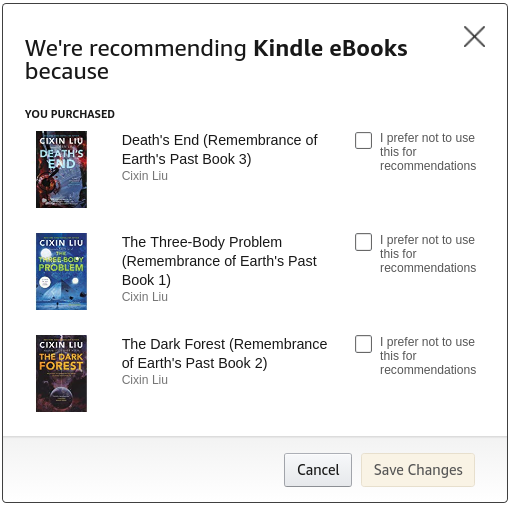
\includegraphics[scale=0.5]{img/AmazonExplanation.png}
    \caption{Amazon's web-page window that provides context why was a particular book recommended.}
    \label{fig:amazon_explain_book_recommendation}
\end{figure}

\begin{figure}[htbp]
    \centering
    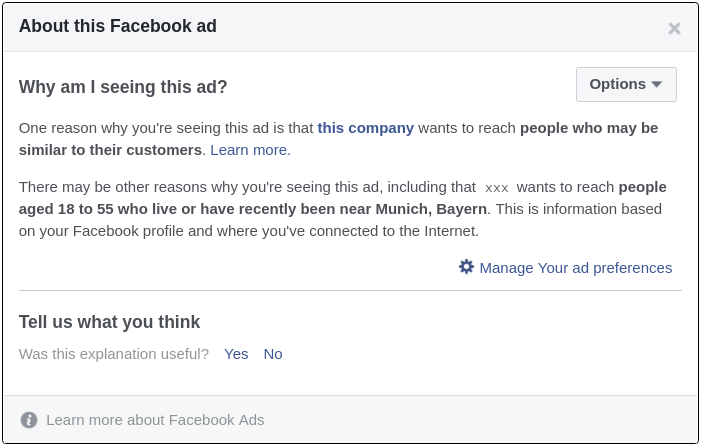
\includegraphics[scale=0.5]{img/FacebookAdExplanation2.png}
    \caption{Facebook's web-page window that provides information about what data lead to user's seeing Facebook's ads.}
    \label{fig:facebook_explain_book_recommendation}
\end{figure}

\subsection{Legitimacy}
Legitimacy can be viewed as an another step after explainability. When we provide a prediction together with a sound reasoning that can be verified either by a human analyst or by an other trusted system, then we can use it in more serious and sensitive deployments. One of them can be the legal domain. In it, computer systems can be used to provide unbiased and fair decisions and analysis, if set up correctly. But as mentioned many times before, we need to be very careful with the data that we use for training. Lot of care needs to be taken even if we do not use an automated training solutions. Most of the current systems used in the mentioned legal domain and other systems where legitimacy is required are most probably base on hand crafted rules that can very well be subject to bias as well. One of the examples being the system COMPAS presented in \ref{subsec:02_algo_fairness.examples_of_algo_biass}.

%\subsection{Auditability}
%\todo[inline]{Add 'Auditability?'}



\subsection{Consistency}
% \todo[inline]{Proc tahle uvodni veta? R: Protoze jsem to bouchal rychle jak hladovej datel :D :| a neprecetl si to po sobe.}
% \todo[inline]{tady vysvetli o jakou novelty ti jde - z kontextu bych tipoval, ze novelty ve smyslu davat na stejny input vzdy trochu jine doporuceni, protoze ty predchozi uz uzivatel videl, ale ani ja si tim nejsem jisty}

For some systems it is very important to stay consistent in outputs even with a slightly different inputs. Lets assume, that we are developing an illness detection algorithm, that offers medical personnel some insights about their patients based on provided symptoms. The predicted recommendation should not drastically change if for example the temperature changes by 0.1°C. It is therefore closely tied to the previous properties of legitimacy and explainability. Most high critical ML systems have to be designed with consistency in mind. Driver-less cars that abruptly change direction with only one pixel change in the input would not induce trust of its users.

From a different perspective we can view fairness as a sort consistency in the way that protected attributes of people do not have an effect on the output, the algorithm is consistent in respect of these protected attributes.
% \todo[inline]{Tady bys mohl zminit ze to souvisi i s fairness v tom ohledu, ze klicove protected atributy lidi by nemely mit vliv na vysledek -> alg. je vuci nim konzistentni. R: To je moc pekny osli mustek.} 

% From less high critical systems we can mention navigation properties in software and recommendation. We sometimes need machine learning user-tailored systems that are exceptional for speeding up work or retrieval of information, but its users would not be comfortable with often changes in the provided recommendations. 

One other meaning of consistency in regards to ML systems can be stability in the meaning of ML outputs being the same while navigating a system or an app. We can attribute it to the application's design more than the ML system it self. If a user is browsing a web page, lets say an aggregator of products on the web, they may rely on the back button while browsing the different outputs. In this setting, inconsistency and changes to the recommendation items may be harmful as it will affect the user experience while listing and using the provided information.

\subsection{Novelty}
Novelty can have multiple meanings when we use it to describe RS. Firstly it can be that the item it self is a new addition to the data-set and we do not have many user-item interactions which we would use to asses and recommend the new item.

Secondly, we can say that the the item is presented to the user for the first time. Sometimes, depending on the presentation of the recommended items, we have to show the recommended item repeatedly in order for it to be noticed. In that way, novelty can be viewed as a non binary attribute, where each time we present the item to the user it decreases the items novelty, with respect to that one user. But often it is viewed as a binary attribute, shown or not-yet-shown.

Thirdly, by novelty we can describe that an unusual item is presented to the user. Such situation can occur either due to the RS incorrectly assuming that the user will like that item, or by, on purpose introducing a new not yet seen item so that we introduce more exploration and present items that the user will view as fresh.

And lastly, novelty is important as an exploration. RS should try to broaden and expand the model of users' preference, which needs to be done by gathering feedback on items outside of the users current preference model. Balance between exploration and exploitation is difficult, but can substantially increase models' performance if done correctly.

In general and contrary to the previously mentioned consistency parameter, we usually strive for novelty and exploration. If a person is picking out a movie to watch, then showing them the same selection over and over would most certainly lead to their dissatisfaction due to the limited and repeated content that the system is providing. As with all properties, novelty requirements heavily depend on the domain the system is deployed in. This property is most sought for in domains where exploration is important.




% As an example, we can imagine that in a movie recommender system a user only watched Harry Potter movies, then a RS that does not try to introduce new novel items will only recommend other Harry Potter movies which will most probably be seen as boring, repetitive and valueless.


% 3 meanings
% new item in dataset
% new item presented to user
% unusual item presented to user
% item that wasn't shown to the user that many times



Contrary to the previously mentioned consistency parameter, we sometimes strive for novelty and exploration. If a person is picking out a movie to watch, then showing them the same selection over and over would most certainly lead to their dissatisfaction due to the limited and repeated content that the system is providing. This property is most sought for in domains where exploration is important.



% \todo[inline]{Zrovna pro novelty existuje celkem dost docela zajimavych interpretaci, ktere se daji zminit. Novelty jako inverse popularity (pokud nemame zaznamy o impressions, interakcni novelty - uzivateli jsme to zatim (mockrat) nezobrazovali, temporalni novelty - je to nove vytvoreny produkt}

\subsection{Coverage}
% Popsat situaci kde rs failuje v tom, ze nejake itemy jsou unreachable, nebudou pak doporuceny vsem, pripadne muzeme taky zminit to, ze popularni itemy budou vzdycky ve vyhode ktera nemusi byt uplne fair v tom, ze kdyz mas exposure tak je jednodussi dostat dalsi exposure, takovej trochu negative feedback loop. A muze se pak stavat, ze misto toho abychom doporucili item ktery je opravdu awesome pro toho uzivatele tak doporucime neco no neni tak awesome

In some ML and RS applications, there can emerge a situation where some items are never recommended. If the reason is that the item quality is bad then it can be the right system quality. In other situations, such as RS that recommends based on item properties, an undesirable behavior can occur when an item is just too different and we do not have a reasonable 'link' to other items that would serve as comparison for the recommendation. Then this item will be left out and never recommended.

Other coverage problem is with items that are popular. Popularity is sometimes a good indicator of quality, but not always. If an item is popular, then in a system that exploits popularity, it will receive more and more attention. This in turn further increases its popularity. In a way we can have a same type of phenomenon as Negative feedback loop mentioned in \ref{subsubsec:02_algo_fairness.adverse_effects.nfl}. It then happens that item exposure distribution will be unnaturally skewed even more towards the popular items. This can lead to decrease in system's performance due to some items that are less popular not being recommended even if being possibly a better choice for recommendation. In a way popularity and unpopularity correspond to a notion of novelty where instead of considering a single user we consider all users of the system together.

% \subsection{Diversity and similarity}
%

\subsection{Efficacy, accuracy and precision}
We have so far mentioned multiple other criteria. But all of them are hard to measure due to their somewhat subjective nature, let us now present two of the most widely used exact efficacy properties: accuracy and fairness.

Accuracy (sometimes as trueness) is a measure of how far away outputs of a ML system are from the desired outputs. Precision is a measure of how unsure or dispersed the outputs are, in other words how away are from each other. They are both measures of observation error and the definitions differ based on type of the systems outputs. We can see an illustration for continuous value prediction on \ref{fig:accuracy_fairness}

\begin{figure}[htbp]
    \centering
    \includesvg[width=9.5cm]{img/accuracy_and_precision.svg}
    \caption{Illustrative description of the relationship of accuracy and precision from \cite{Accuracy_precision}}
    \label{fig:accuracy_fairness}
\end{figure}

How to measure the distance of outputs to ground truth can differ based on the shape/dimensionality of the output. Usually we use a simple metric such as Euclidean distance or simple Manhattan distance.


For categorical data we have (binary retrieval task and multi-class classification respectively):
\begin{equation}
    Accuracy = \dfrac{\text{TP + TN}}{\text{TP + FP + TN + FN}} = \dfrac{\text{correct classifications}}{\text{all classifications}}
\end{equation}
and precision for binary classification:
\begin{equation}
    Precision = \dfrac{\text{TP}}{\text{TP + FP}}
\end{equation}

Precision for categorical data does not have a set meaning, we can either use precision for each class separately or have one class that act as a FP label.

Difficulties with using accuracy arise when miss labels to some or all items in the dataset. Calculating the correct denominator in categorical case or the correct distance to the reference value can be difficult or and impossible.

\subsection{Performance and scalability}
% Popsat motivaci teto sub, performance vice vyznamu, total resources needed, odezva, availability, scalability, one computer nezvladne uplne vsechno co si vymyslim
We can design any algorithm we want, but what for will it be if cannot then use it in the real world? Theoretical algorithms certainly have their place, but we are aiming to solve real problems of addressing fairness. Therefore another and last discussed property will be performance and with it related property of scalability.

Performance of as system can be described either in a form of total computational resources needed for processing, either the whole deployment or normalized to a single user. Other possible performance property can be the length of time needed for processing of a single request called latency. These two properties usually need to be balanced against each other. To a certain point we can either add more computational capacity to improve - decrease latency, or remove some capacity with the possible increase in latency.

Scalability is a property of a system that the it is able to handle a growing amount of work. We have to keep this property in mind while designing ML and RS systems. If for example we are using a comparison with other users such is the case in some RS algorithm, we will be growing the system requirements most probably linearly with the amount of users. This can be fine in for example research applications, but becomes a real concern when applying to a world wide applications used by millions of users. At these scales we will be required to scale using not only vertical scaling (that is using a more powerful computational resources), but mainly using horizontal scaling (by using many computers at once).



% \todo[inline]{Z toho co tu jsou jen jako nadpisy, tak diversity a similarity mi trochu splyvaji, podobne precision a accuracy - minimalne vzhledem k tomu ze jsi o ostatnich vecech mluvil na dost high-level urovni, tak bych tohle asi spojil dohromady.}


% TODO: Fairness is not the only property we can try to manage, what about privacy, accuracy, precision, coverage, diversity, novelty and so on. Mention them first in an overview, then separately in subsections in more detail. Try to define them mathematically.

\chapter{Related work} \label{chap:related_work}
In this chapter, we will go in-depth discussing common approaches that are being used in the group recommendation task. First, specifying the main approaches, dividing them into groups by how they approach the transition from single-user preferences to group results. Then mentioning the main simple techniques and describing how they interact with the common recommendation approaches. And at last diving into some of the more advanced methods that optimize the aggregation in a more elaborate way.

\section{Categories} \label{sec:03_categories}
We assume that we have individual user preferences (if group preferences are available, then the task actually becomes a simple recommendation with the group acting as a single user), therefore it is necessary to make a distinction based on where the algorithm goes from the preference of the group's individual users to a result for the whole group.

We can put each algorithm into one of the following three groups based on the aggregation step:
\begin{itemize}
    \item \textbf{Aggregate models} \newline
    The aggregation works on merging the preferences of each member of the group into a single set of preferences that can be then directly consumed by a recommender system, therefore creating a group preference model. Aggregating the single-user preferences either directly by aggregating ratings of seen, or and rated items, or by aggregating the extracted models of user preference to create a single model for the whole group, such as preference matrix in matrix factorization approaches, text descriptions, or item-based recommendations and so on, we will discuss these techniques later.
    
    % Aggregates the models for RS. Recommender is working on a set of already aggregated group preferences, either directly aggregating ratings of seen items, or more high level extracted features such as preference matrix in matrix factorization approaches, text description for item-based recommendations and so on, we will discuss these techniques later.
    
    This aggregation step precedes the recommendation step. We can see a visualization in figure \ref{fig:before_rec_agg}.
    
    
    \item \textbf{Aggregate predictions} \newline
     Aggregates predictions outputted from RS. Recommender recommends separately for each member of the group based solely on their single-user preferences. Then the resulting recommended items are aggregated together to a single list of recommendations for the whole group. There are two main ways how the final list can be created. Either directly take items recommended to each user and append them together in some specified manner, or the second way, calculate some common utility function from all recommended items and select those that are the most fitting to the group based on this utility function. We will discuss both in more detail in the section \ref{sec:03_simple_aggregation_metods}.
     
     The aggregation step follows after the actual recommendation step. We can see a visualization of this approach in figure \ref{fig:after_rec_agg}.
     
    \item \textbf{Aggregation is a uniform part of the recommender} \newline
    In this case, the algorithm directly works with users of the group and does not allow for a clear distinction of the aggregation step. It is deeply and inseparably built into the algorithm itself. Sometimes the perception of the inseparability of these two steps can vary in the literature. Some could say that for example aggregating the user profiles in matrix factorization makes the aggregation inseparable, because there is a specific preprocessing done before the aggregation step. But others will point out, that the user latent matrix is just a representation of a user preference, even if processed by the algorithm itself. We will let the reader decide for themselves where they see the distinguishing border. We will briefly discuss the available methods in section \ref{sec:03_advanced_methods}
\end{itemize}


This presented grouping based on the aggregation step is different from the main literature  \cite{recommendations_to_groups-jameson2007} and \cite{grouprecommendersystems_felfernig2018group}, where they also make a distinction into three groups, but instead based on the data that the aggregation processes and the position. Instead we have chosen a little different distinction based more on interaction of the aggregation with the recommender system, essentially putting two groups from aforementioned literature under single group (\textit{aggregate models}), but with the mentioned possible subdivision.
    

\begin{figure}[htbp]
    \centering
    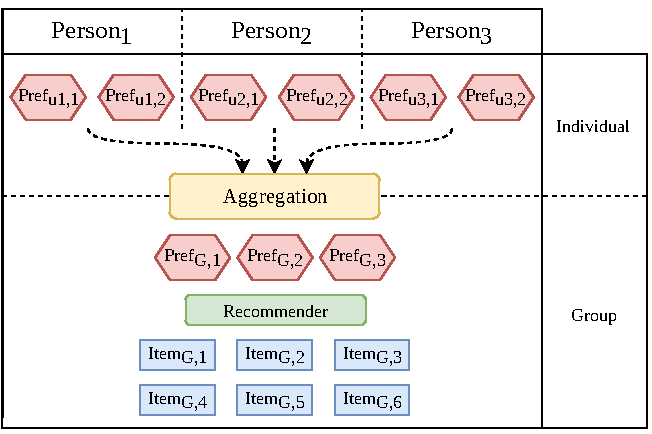
\includegraphics{img/before-rec-aggregation.pdf}
    \caption{High level overview of group recommendation with aggregation of individuals' preferences, before recommendation.}
    \label{fig:before_rec_agg}
\end{figure}

\begin{figure}[htbp]
    \centering
    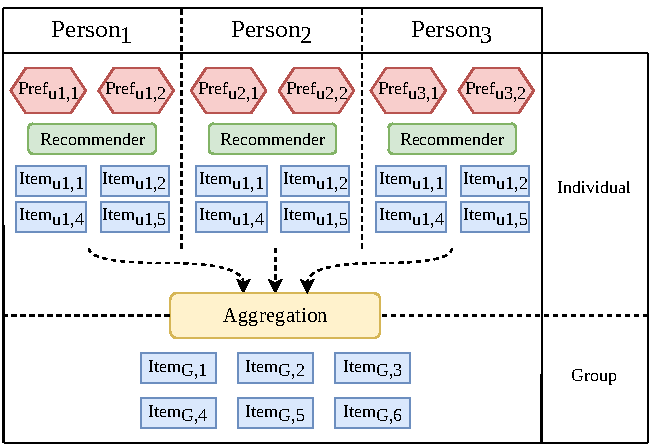
\includegraphics{img/after-rec-aggregation.pdf}
    \caption{High level overview of group recommendation with aggregation on top of recommendation results for individual users.}
    \label{fig:after_rec_agg}
\end{figure}






\section{Simple aggregation methods}\label{sec:03_simple_aggregation_metods}
We will now introduce the main aggregation functions (interchangeably as "aggregation strategies", "aggregation methods") used, together with an overview of how they interact with the single-user recommender systems introduced in chapter \ref{subsec:01_rec_sys.main_alg_approaches}
\subsection{Methods}\label{subsec:03_simple_aggregation_methods.methods}

The main aggregation methods can be divided into three groups, based on their high-level approach into - majority, consensus, and borderline based strategies. The majority-based generally use the most popular item among the group members, the consensus-based consider preferences of all the group members, and the borderline-based consider a subset of the items by some limiting criteria.

We now list the most common aggregation methods as mentioned in \cite{grouprecommendersystems_felfernig2018group}, \cite{masthoff_2011_group_rec_systems} and \cite{masthoff_2004_group_modeling} specify to which of the group mentioned above they belong.
%The common aggregation methods as mentioned in \cite{grouprecommendersystems_felfernig2018group}, \cite{masthoff_2011_group_rec_systems} and \cite{masthoff_2004_group_modeling} are:

\begin{itemize}
    \item \textbf{Additive utilitarian} (ADD, consensus)\newline
        Sum of scores for an item across the group
        \begin{equation}
            \argmax_{i \in I}{\sum_{u \in G}{\textrm{score}(u,i)}}
        \end{equation}
    
    \item \textbf{Approval Voting} (APP, majority)\newline
        Number users that like the item above a certain threshold
        \begin{equation}
            \argmax_{i \in I}{
                \big\lvert{\left\{
                    u \in G : \textrm{score}(u,i) \geq \textrm{treshold}
                \right\}}\big\rvert
            }
        \end{equation}
    
    \item \textbf{Average} (AVG, consensus)\newline
        Average of scores for an item across the group
        \begin{equation}
            \argmax_{i \in I}{\dfrac{\sum_{u \in G}{\textrm{score}(u,i)}}{\abs{G}}}
        \end{equation}
    
    \item \textbf{Average without Misery} (AVM, consensus)\newline
        Average of scores for an item across the group only if the item is above a certain threshold for all group members
        \begin{equation}
            \argmax_{ i \in I : \nexists u \in G | \textrm{score}(u,i) \leq \textrm{treshold}}{
                \dfrac{\sum_{u \in G}{\textrm{score}(u,i)}}{\abs{G}}
            }
        \end{equation}
        
    \item \textbf{Borda count} (BRC, majority)\newline
        Sum of scores derived from item rankings. The ranking score is defined for each user by ordering the user's items by score and awarding points corresponding to the location of the item in this ordered list. Worst item receiving 1 point and best item $|I|$ points.
        \begin{equation}
                \argmax_{i \in I}{\left(\sum_{u \in G}{\textrm{RankingScore}(u,i)}\right)}
            \end{equation}
        Where \textit{ranking score} is defined as follows:
        \begin{equation*}
            \textrm{RankingScore}(u,i) := 
            \big\lvert{\left\{
                i_{other} \in I : \textrm{score}(u,i_{other}) \leq \textrm{score}(u,i)
            \right\}}\big\rvert
        \end{equation*}
    
    \item \textbf{Copeland rule} (COP, majority)\newline
        Difference between number of wins and losses for pair-wise comparison of all items
        \begin{equation}
            \argmax_{i \in I}{
                \big(\textrm{W}(t, I - t) - \textrm{L}(t, I - t)\big)
            }
        \end{equation}
    
    \item \textbf{Fairness} (FAI, consensus)\newline
        Users, in turn, one after another select their top item.
        \begin{equation}
            \argmax_{i \in I}{{\textrm{score}(u_{current},i)}}
        \end{equation}
        Where $u_{current}$ is user selected from $G$ for each iteration according to some (in most cases circular, or ping pong) rule.
    
    \item \textbf{Least misery} (LMS, borderline)\newline
        Uses the lowest received rating among the group members as the item's aggregated rating.
        \begin{equation}
            \argmax_{i \in I}{\left(\min_{u \in G}{\left(\textrm{score}(u,i)\right)}\right)}
        \end{equation}
    
    \item \textbf{Most Pleasure} (MPL, borderline)\newline
        Uses the highest received rating among the group members as the item rating.
        \begin{equation}
            \argmax_{i \in I}{\left(\max_{u \in G}{\left(\textrm{score}(u,i)\right)}\right)}
        \end{equation}
        
    \item \textbf{Majority Voting} (MAJ, majority)\newline
        Uses the rating that was given by the majority of the group's members. (Can only work on discrete ratings)
        \begin{equation}
            \argmax_{i \in I}{\left(\mode_{u \in G}{\left(\textrm{score}(u,i)\right)}\right)}
        \end{equation}
    
    \item \textbf{Most Respected Person} (MRP, borderline)\newline
        Uses rating proposed by the most respected member of the group.
        \begin{equation}
            \argmax_{i \in I}{\textrm{score}(u_{most\_respected},i)}
        \end{equation}
        
        
    \item \textbf{Multiplicative} (MUL, consensus)\newline
        Multiplies all received ratings together.
        \begin{equation}
            \argmax_{i \in I}{\left(\prod_{u \in G}{\textrm{score}(u,i)}\right)}
        \end{equation}
        
        
    \item \textbf{Plurality Voting} (PLU, majority)\newline
        Each user has a set number of votes that get distributed. The item with the most received votes is selected.
        \begin{equation}
            \argmax_{i \in I}{\left(\sum_{u \in G}{\textrm{VotesAwarded}(u,i)}\right)}
        \end{equation}
        
        Where \textit{votes awarded} is some function that decides for each user how the available votes will be distributed among the items.
        
\end{itemize}

Some of the methods have an additional distinguishing factor, which is that they are iterative calculations instead of a single calculation that returns the final ordering. Most notably \textit{Fairness}, it calculates the next item purely from a currently selected user, users changing in iterations one after another. Another one is \textit{Plurality Voting}, this technique can also be iterative but it is not mandatory. Where after the top item is selected we reset the calculation, therefore selecting top items in an iterative manner. All the other ones are single-iteration methods, where the final list requires only one calculation.

Now we will show how these strategies work together with a recommendation in order to provide a full group recommender system, which will serve as an introduction of the inner workings of such system in order for us to then continue towards more advanced aggregation methods.

\subsection{Usage with recommender systems}
We now need to distinguish between \textit{model aggregation} and \textit{prediction aggregation} due to in most cases very different inputs and required outputs from the aggregation.
\subsubsection{Prediction aggregation}
In most cases using them as \textit{prediction aggregation} after the recommendation is quite straightforward. In all (to us known) cases RS returns recommended items together with some sort of rating of the recommendation. There are some applications where this presumption does not hold, such as building a group recommendation aggregation on top of a \textit{black box} recommender that only returns a list of items, for example, if extracting recommended items data from a web page where we only retrieve the list itself and we do not have access to the underlying recommender system. But in the following section we will assume that we have a full access to the rating data of the outputted items. We further assume that if necessary we can acquire ratings and ordering for all possible items.

As shown in figure \ref{fig:after_rec_agg}, we first get a list of recommended items (together with ratings) for each user. Then we can directly apply the methods mentioned in section \ref{subsec:03_simple_aggregation_methods.methods}.

\subsubsection{Model aggregation}
Running aggregation on top of user preferences, instead of lists of recommended items is more challenging due to many possible inputs that the recommender can take, such as explicit or and implicit feedback. As discussed in section \ref{sec:03_categories}, we have two main options, aggregation of ratings and aggregation of mined preferences.

First, the aggregation of ratings, in other words creating a set of ratings that represent the whole group. This approach is preferred due to its simplicity. We can use many of the before mentioned simple methods, mainly the \textit{consensus-based} which aggregate ratings directly (positive as well as negative ratings). Other mentioned methods can be used as well, but some of them do not make much sense to adapt, for example, the voting-based, with which we will be very limited due to the usual sparsity of the feedback ratings that we have available.

The second option, the aggregation of mined preferences, is more present in content-based systems. Where we aggregate not the rating themselves but some other data that represent the users' likes and dislikes. As an example, we will use the \textit{tf-idf} keyword extraction which is by far the most popular method used in the text-based recommendation as mentioned in \cite{beel_2016_rs_literature_survey}. We can weight \textit{tf-idf} concepts extracted from the user feedback by the received rating, and then aggregate these concepts together for the whole group. As we can see, it is a little more elaborate approach that requires more modifications to the simple methods mentioned.

%The above mentioned aggregation methods can be used with collaborative filtering, mentioned in \ref{subsec:01_group_rec_sys.common_aproaches}, as a \textit{model aggregation method} (Fig. \ref{fig:before_rec_agg}) as well as a \textit{prediction aggregation method} (Fig. \ref{fig:after_rec_agg}). As already mentioned the method is based on the idea of recommending items that were liked by users with similar preference. First we mention how \textit{prediction aggregation} works with collaborative filtering.

%\section{Advanced aggregation methods}\label{sec:03_advanced_aggregation_methods}
\section{Advanced methods}\label{sec:03_advanced_methods}
As we can see, the simple methods mentioned before are quite straightforward, they have mostly very simple and clear objectives, and try to optimize in different ways some quite vaguely specified goal. But as we have discussed in the chapter \ref{chap:fairness}, the objective is quite hard to define and measure. We will now introduce some other methods that either directly or indirectly try to optimize some better-specified goal.

\subsection{GFAR} \label{subsec:03_advanced_methods.gfar}
So far we have introduced methods that do not directly specify any form of optimization in a direction of \textit{fairness}. A new method introduced in\cite{GFAR-kaya2020} directly optimizes the resulting list to balance the relevance of the recommended items in a rank-sensitive way.

\subsubsection{Introduction}

As mentioned they focus on the \textit{fairness} of top-$N_G$ (\textit{fairness} of the top N recommended items for the group G). Where they define \textit{fairness} as a property of the top-$N_G$ items, not just any single item but the whole list. As already discussed in chapter \ref{sec:01_rec_sys} the difference between optimization independently item after item versus in some way for the whole list can yield significantly better results when it comes to sequential consumption of items or and balancing users with different preferences. For example, being one member of the group being treated unfairly due to different preferences from the rest of the group, then fairness defined as a property of the whole list can in some way compensate and give more priority for balancing fairness forwards this one user. This kind of unfairness is the main problem that they try to solve.

We have already mentioned one algorithm that tries to balance fairness of the whole list in chapter \ref{subsec:03_simple_aggregation_methods.methods}, FAI, which generates the aggregated results in iterations, each iteration optimizing for a different user in turns. This approach solves the aforementioned problem in a very simple (although somewhat dull) way by not considering the group preferences at all and just trying to please everyone in turns not considering if the item will be liked by the rest of the group.


\subsubsection{Approach}

What if we have instead taken into account the previously recommended items when we are selecting the next one in the list? The authors propose defining \textit{fairness} together with ordering within the group by saying that "a top-$N$ is fair to a group if the relevance of the items is balanced across the group members for \textit{each prefix} of the top-$N_G$". In other words for each iteration, we try to select an item that improves the balance as much as possible.

Let us first define Borda relevance following \cite{xiao_2017_fairness_aware_g_rec} as:


% In original paper there is an error in the direction of </>
\begin{equation}
    \textrm{Borda-rel}(u,i) = 
    \big\lvert{
        \left\{j : \textrm{rank}(j, \textrm{top-}N_u) < \textrm{rank}(i, \textrm{top-}N_u) \right\}, \forall_j \in \textrm{top-}N_u)
    }\big\rvert
\end{equation}

Where rank is the position of item $i$ in the user's $u$ candidate list (position is determined by ordering the items based on the returned items score, from the best to the worst). Borda relevance essentially gives zero points to the last item and increases the points by one for each position up in the list, with the first/top item getting $(\#\textrm{items} - 1$) points.

Now we can set probability of item $i$ being relevant for user $u$ as:

\begin{equation}
    p(\textrm{rel}|u, i) = \frac{\textrm{Borda-rel}(u, i)}{\sum_{j \in \textrm{top}-N_u}{\textrm{Borda-rel}(u, j)}}
\end{equation}

Let also $p(\neg\textrm{rel}|u, S)$ be the probability that item $i$ is not relevant for any of the items in set $S$. We derive the probability that atleast one item from set $S$ is relevant to the user $u$ as:

\begin{equation} \label{eq:atleast_one_relevant}
\begin{aligned}
    p(\textrm{rel}|u, S) &= 1 - p(\neg\textrm{rel}|u, S) \\
    & = 1 - \prod_{i \in S}{(1 - p(\textrm{rel}|u, i))}
\end{aligned}
\end{equation}

Now we want to generalize for the whole group, so we define $f(S)$ as the sum of probabilities for each user that they find at least one relevant item in the set $S$:

\begin{equation} \label{eq:relevance_for_set}
\begin{aligned}
    f(S) &= \sum_{u \in G}{\left(1 - p(\neg\textrm{rel}|u, S)\right)} \\
    & = \sum_{u \in G}{\left(1 - \prod_{i \in S}{(1 - p(\textrm{rel}|u, i))}\right)}
\end{aligned}
\end{equation}

We have used the Group G as a constant in equation \ref{eq:relevance_for_set} and forward, the group will stay the same during the calculation. $f(S)$ shows how to balance the fairness amongst the group members for a specified set of item. We now want to extend it in order to make it rank-sensitive by defining a marginal gain in function $f$ for adding a new item $i$ to the set $S$ as follows:

\begin{equation} \label{eq:relevance_for_set_add}
\begin{aligned}
    f(i, S) &= f(S \cup {i}) - f(S) \\
    & = \sum_{u \in G}{\left[p(\textrm{rel}|u, i) \prod_{j \in S}{(1 - p(\textrm{rel}|u, j))}\right]}
\end{aligned}
\end{equation}

Where we have used equations \ref{eq:atleast_one_relevant} and \ref{eq:relevance_for_set}. And finally, we can define an ordered set that is considered fair if it balances each of its prefixes. In other words, the first item of the set should be considered fair/balanced by all group members as much as possible, then the first two items and so on, we define fairness in an ordered set $OS$ as:

\begin{equation}
    \textrm{fair}(OS) = \sum_{k=1}^{|OS|}{f(OS)[k], \{i \in OS : \textrm{rank}(i, OS) < k\})}
\end{equation}


\subsection{Package-to-Group Recommendations}
Paper \cite{serbos_2017_fairness_packages_to_group_rec}?


\subsection{Top-N group RS with fairness}
Paper \cite{sacharidis_2019_top_n_with_fairness}?
% TODO:
% - Make a tool for download and transformation of datasets, and sell the work that I have done
% - Compare single user datasets
% - group rec datasets mention
% - do dataset group augmentation and add it to the tool


\chapter{Datasets}  \label{chap:datasets}
People are gregarious in nature, but the same, unfortunately, cannot be said about machine learning datasets. Vast majority of them are not directly usable in the group RS research due to only containing information about single user preference. In order to design and evaluate group recommender systems, we preferably need datasets that contain information about groups' preference.

In this chapter, we will start with description of which datasets are suitable for the use in RS domain. We describe commonly used datasets in the non-group RS domain. Analyse their high level properties and describe what transformations are needed in order to make the use of the dataset convenient. 

Next, we will talk about the existing group RS datasets and introduce methods that can be used to generate the group recommendation information synthetically from non-group RS datasets. We will use these methods to generate standardized synthetically enriched group RS datasets from non-group datasets that we will describe in the single user datasets subchapter.

And finally, we describe a data transformation library that we create for the purpose of simplifying the research efforts in the RS domain and for evaluation of our proposed algorithm.

% We will first describe a few of the popular datasets which we have determined to be used as research data the most. Then we will 

% -------------------------------------------------------------------------------------
\section{Single user datasets} \label{sec:single_user_datasets}
% -------------------------------------------------------------------------------------
Multiple well known and thoroughly studied datasets exist in the recommender system domain. Let us now present the popular ones that seems to be utilized the most.

If we talk about specific format of the data then we are referring to the unified format which we have transformed the original data into using the dataset transformation library. Further description about the data format transformations follow in \ref{subsec:04_single_user_datasets.gathering_processing}.



% -------------------------------------------------------------------------------------
\subsection{Movie Lens}
% -------------------------------------------------------------------------------------
One of the most well known dataset in the RS domain, it contains 25 million ratings in total across 62,000 movies and 162,000 users. The data were collected between 1995 and 2019 and the current version of this size (25M) was released in November of 2019. Data are organic and come from a web-based recommendation system at \href{https://movielens.org/}{movielens.org}. The project was specifically created in order to gather research data on personalized recommendation by researches at University of Minnesota.

Dataset is in a good format that is quite easy to parse and use. Further description follows in \ref{subsec:04_single_user_datasets.gathering_processing}.

\hfill \break
\noindent
\textbf{Number of items:} 62,000 \newline
\textbf{Number of users:} 162,000 \newline
\textbf{Number of user-item interactions:} 25,000,095 \newline
\textbf{User-item interactions format:} Sparse matrix of ordinal ratings [1, 1.5, 2, ... 4.5, 5] - user rated a movie \newline
\textbf{List of datatables:} Movies (detail in Table \ref{table:5.1_ML_movies}), Ratings (detail in Table \ref{table:5.1_ML_ratings}), Tags, Links, Genres, Genome Scores, Genome Tags

\begin{table}[ht!]
\centering
\begin{tabular}{ l l }
\verb|item_id| & \verb|title| \\
    \hline
     1  &                   Toy Story (1995) \\
     2  &                     Jumanji (1995) \\
     3  &            Grumpier Old Men (1995) \\
   ...  &                                ... \\
209169  &                A Girl Thing (2001) \\
209171  &     Women of Devil's Island (1962) \\ [1mm]
\multicolumn{2}{l}{{[62423 rows x 2 columns]}}
\end{tabular}
\caption{Short snippet of Movie Lens dataset's \texttt{movies.csv} table.}
\label{table:5.1_ML_movies}
\end{table}

\begin{table}[!ht]
\centering
\begin{tabular}{ l l l l }

% \texttt{user\_id} & \texttt{item\_id} & \texttt{rating} & \texttt{timestamp} \\
\verb|user_id| & \verb|item_id| & \verb|rating| & \verb|timestamp| \\
    \hline
    1 &      296  &   5.0 & 1147880044 \\
    1 &      306  &   3.5 & 1147868817 \\
    1 &      307  &   5.0 & 1147868828 \\
  ... &      ...  &   ... &        ... \\
162541 &    58559  &   4.0 & 1240953434 \\
162541 &    63876  &   5.0 & 1240952515 \\ [1mm]
\multicolumn{4}{l}{{[25000095 rows x 4 columns]}}
\end{tabular}
\caption{Short snippet of Movie Lens dataset's \texttt{ratings.csv} table.}
\label{table:5.1_ML_ratings}
\end{table}

% This dateset contains information about movies in the form of \textit{'\textless movieId, title, genres\textgreater'}, ratings in the form of \textit{'\textless userId, movieId, rating, timestamp\textgreater'} and additional information about links, tags, genome-scores and genome-tags.




% -------------------------------------------------------------------------------------
\subsection{KGRec}
\label{subsec:04_single_user_datasets.kgrec}
% -------------------------------------------------------------------------------------
KGRec is a smaller and less known dataset. We have chosen this dataset because it was utilized in GFAR method introduced in \cite{GFAR-kaya2020} and described in \ref{subsec:03_advanced_methods.gfar}. This dataset consists of two separate datasets of music and sound, KGRec-music and KGRec-sound respectively.

The first music dataset comes from \href{https://www.songfacts.com/}{songfacts.com} (items and text descriptions) and \href{https://www.last.fm/}{last.fm} (ratings, items, tags). Each user-item interaction is a user listening to a song.

The second, sound dataset, comes from \href{https://freesound.org/}{freesound.org}. Items are sounds with description using text and tags that were created by the person that uploaded the sound. Each user-item interaction is a user downloading an item, in this case a sound.

Further, we will consider only the music dataset and not utilize the sound dataset at all. We have made this decision to simplify comparisons and due to the origin of the sound dataset itself. It comes from a web-page where users can upload and download random sounds of their choosing, such as 'Mechanical clock movement' sound, 'Industrial elevator' sound and so on. The need for these sounds are most probably driven from people that are using them for their profession, such as video production and therefore does not reflect natural content consumption preferences.

Both datasets were created for the needs of \cite{kgrec_dataset_origin}, where they were introduced, they are altered for the needs of research in Recommendation Knowledge Graphs. Further, the original data that were used for creation of this datasets are described in \cite{kgrec_dataset_origin_full}.


\hfill \break
\noindent
\textbf{Number of items:} 8,640; 21,552\footnote{Number of items, users and user-item interactions are in order - music dataset; sound dataset} \newline
\textbf{Number of users:} 5,199; 20,000 \newline
\textbf{Number of user-item interactions:} 751,531; 2,117,698 \newline
\textbf{User-item interactions format:} one-valued implicit feedback - user listened or downloaded a song/sound \newline
\textbf{List of datatables:} Ratings(detail in Table \ref{table:5.1_KGRec_ratings}), Tags, Descriptions

\begin{table}[!ht]
    \centering
    \begin{tabular}{ l l }
        \verb|user_id|   & \verb|item_id| \\
        \hline
        7596     &  68  \\
        7596     & 130  \\
        7596     & 330  \\
        ...      & ...  \\
        50572897 & 8618 \\
        50572897 & 8619 \\ [1mm]
        \multicolumn{2}{l}{{[751531 rows x 2 columns]}}
    \end{tabular}
    \caption{Short snippet of KGRec dataset's \texttt{music\_ratings.csv} table.}
    \label{table:5.1_KGRec_ratings}
\end{table}

% \newline
% Both dataset are in the form of '\textlessuser userId, itemId\textgreater'


% -------------------------------------------------------------------------------------
\subsection{Netflix Prize}
% -------------------------------------------------------------------------------------

Data that were originally released in 2009 by the Netflix.com video streaming company for the \textit{Netflix Prize}, open competition with main prize of 1 million dollars. It contains data of more than 400 thousand randomly selected users from the company's database. Data contain information about users ratings of movies. It was originally available on the contest web page, but has been removed since.

The original data was split into multiple files in a file for ratings per movie manner. Each rating is a quadruplet of the form '\textless user, movie, date of rating, rating\textgreater'.

\hfill \break
\noindent
\textbf{Number of items:} 17,770 \newline
\textbf{Number of users:} 480,189 \newline
\textbf{Number of user-item interactions:} 100,480,507 \newline
\textbf{User-item interactions format:} sparse matrix of ordinal ratings [1, 2, 3, 4, 5] \newline
\textbf{List of datatables:} Ratings (detail in Table \ref{table:5.1_Netflix_ratings}), Movies (detail in Table \ref{table:5.1_Netflix_movies})

\begin{table}[!ht]
    \centering
    \begin{tabular}{ l l l l }
        \verb|user_id| & \verb|item_id| & \verb|rating| & \verb|date| \\
        \hline
              6 &             30 &             3 &  2004-09-15 \\
              6 &            157 &             3 &  2004-09-15 \\
              6 &            173 &             4 &  2004-09-15 \\
            ... &            ... &           ... &         ... \\
        2649429 &          17627 &             3 &  2003-07-21 \\
        2649429 &          17692 &             2 &  2002-12-07 \\ [1mm]
        \multicolumn{4}{l}{{[100480507 rows x 4 columns]}}
    \end{tabular}
    \caption{Short snippet of Netflix dataset's \texttt{ratings.csv} table.}
    \label{table:5.1_Netflix_ratings}
\end{table}
    
\begin{table}[!ht]
    \centering
    \begin{tabular}{ l l l }
        \verb|item_id| & \verb|release_year| & \verb|title| \\
        \hline
            1 &       2003.0 &            Dinosaur Planet    \\
            2 &       2004.0 & Isle of Man TT 2004 Review    \\
            3 &       1997.0 &                  Character    \\
          ... &          ... &                        ...    \\
        17769 &       2003.0 &                The Company    \\
        17770 &       2003.0 &               Alien Hunter \\ [1mm]
        \multicolumn{3}{l}{{[17770 rows x 3 columns]}}
    \end{tabular}
    \caption{Short snippet of Netflix dataset's \texttt{movies.csv} table.}
    \label{table:5.1_Netflix_movies}
\end{table}
% -------------------------------------------------------------------------------------
\subsection{Spotify - Million Playlist Dataset}
% -------------------------------------------------------------------------------------
This dataset was released in January 2018 for \textit{The Spotify Milion Playlist Dataset Challenge}. It contains 1,000,000 playlists with information about tracks that are part of each playlist. Main purpose of this dataset was to study and develop better algorithms for automatic playlist continuation where the system would be able to recommend songs that are similar to those that are already in the playlist. In contrast to the Netflix challenge, no prize was to be awarded at the end of the challenge.

Even though the context of this dataset are playlists and not users, we utilize a different view on the dataset, where each playlist will represent a single user. This way, we have an another big and organic dataset at our disposal. It can therefore be used not only for playlist continuation tasks, but for the classical RS domain tasks as well. In a sense, a single playlist is a specific subset of preference of the user that have created the playlist. Therefore we expect to see a narrower preference distribution for each of these 'playlist' users.

For completeness, it is necessary to add that some playlists are 'collaborative', meaning that they were created by multiple users. But they account for only 2.3\% of all playlists, which in our opinion does not substantially affect the dataset. These collaborative datasets could be used as a group recommender dataset on their own, unfortunately, the information about which user added which track, to the collaborative playlist, is not present.

\begin{table}[!ht]
    \centering
    \begin{tabular}{ l l }
        \verb|playlist_id|   & \verb|item_id| \\
        \hline
        549000     &  0  \\
        549000     & 1  \\
        549000     & 2  \\
        ...      & ...  \\
        302999 & 133087 \\
        302999 & 133088 \\ [1mm]
        \multicolumn{2}{l}{{[66346428 rows x 2 columns]}}
    \end{tabular}
    \caption{Short snippet of Spotify Milion Playlist dataset's \texttt{ratings.csv} table.}
    \label{table:5.1_Spotify_ratings}
\end{table}


\begin{table}[!ht]
    \centering
    \begin{tabular}{ l l l }
        \verb|item_id| & \verb|item_name| & \verb|artist_name|  \\
        \hline
             0 & Boots of Spanish Leather &         Bob Dylan \\
             1 &       Mr. Tambourine Man &         Bob Dylan \\
             2 &             Danny's Song & Loggins \& Messina \\ 
           ... &                      ... &               ... \\
       2262290 &               Robin Hood &        Crazy Fool \\
       2262291 &                Guilttrip &      Ace Reporter \\ [1mm]
       \multicolumn{3}{l}{{[2262292 rows x 6 columns]}}
    \end{tabular}
    \caption[Short snippet of Netflix dataset's \texttt{tracks.csv} table.]{Short snippet of Netflix dataset's \texttt{tracks.csv} table. (Columns \texttt{item\_uri}, \texttt{artist\_uri}, \texttt{album\_uri}, containing URI to Spotify object were omitted for simplicity due to their substantial length.)}
    \label{table:5.1_Spotify_tracks}
\end{table}

\hfill \break
\noindent
\textbf{Number of items:} 2,262,292 \newline
\textbf{Number of users:} 1,000,000 \newline
\textbf{Number of user-item interactions:} 66,346,428 \newline
\textbf{User-item interactions format:} one-valued implicit feedback - user added a song to a playlist\newline
\textbf{List of datatables:} Tracks (detail in Table \ref{table:5.1_Spotify_tracks}), Ratings (detail in Table \ref{table:5.1_Spotify_ratings})




% -------------------------------------------------------------------------------------
\subsection{Comparison of datasets}
% -------------------------------------------------------------------------------------

\begin{figure}[ht!]
    \centering
    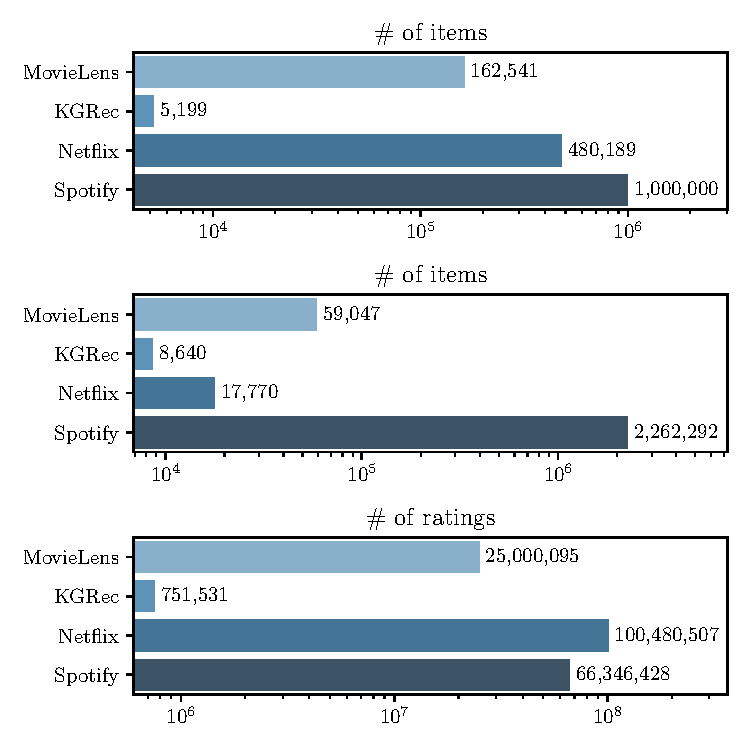
\includegraphics{img/figures/datasets_counts.pdf}
    \caption[Size comparison of the selected datasets.]{Size comparison of the selected datasets. All x-axes are log scale due to the big differences between the dataset.}
    \label{fig:datasets_counts}
\end{figure}

We have described each dataset separately, let us now compare them together to see how they differ. As we can see on Figure \ref{fig:datasets_counts} the Spotify and Netflix datasets are the biggest. We see that KGRec dataset is almost two orders of magnitude smaller than the rest of the datasets. As already mentioned, we have selected it due to it being utilized in the related literature. Spotify dataset is different by having two orders of magnitude more items, which can present a challenge on its own. If we for example use matrix factorization methods to compute the preference, then the amount of memory will rise by two orders of magnitude as well. Additionally, the sparsity of ratings is higher, which can negatively affect efficacy.

Movie Lens dataset has a potential benefit as it has actual ratings for each user-item interaction. All other presented datasets only contain user-item interactions in the form of one-valued implicit feedback.

\begin{figure}[ht!]
    \centering
    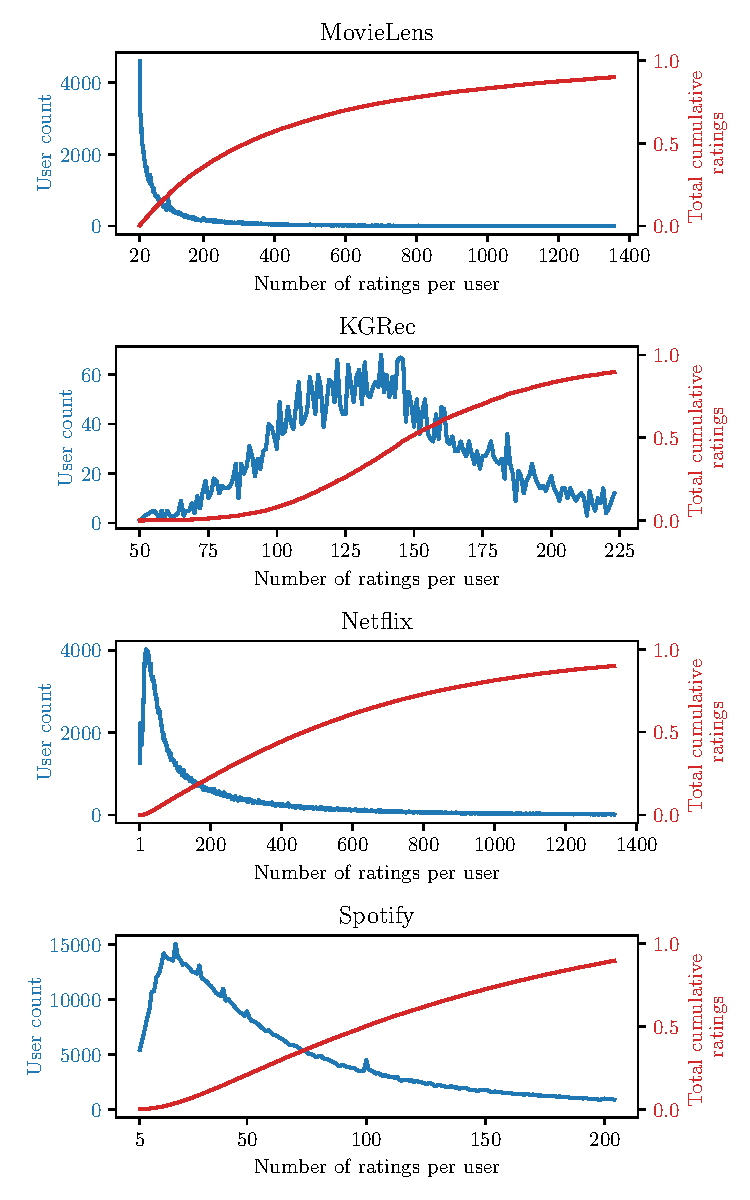
\includegraphics{img/figures/num_users_by_rating_count.pdf}
    \caption[Distribution of ratings]{Distribution of ratings for groups of users by how many ratings they have made. Blue line shows how many users have made that particular amount of ratings, while red line shows the total cumulative mass distribution of ratings. We have clipped the number of ratings by total cumulative ratings of 90\% due to very long-tailed data, where some small amount of users created a very high amount of ratings.}
    \label{fig:datasets_num_ratings}
\end{figure}

On Figure \ref{fig:datasets_num_ratings} we present the distribution of ratings among users. The left y-axis, blue, present count of users with particular number of ratings. We have clipped the users with high number of ratings so that we can better see the interesting part of the data, which would otherwise be squashed by the long tails. The clip was made on the last 10\% mass of all ratings.

We see, that Movie Lens nicely follows a power-law distribution. In this dataset, only users with more than 20 ratings are present which is visible on the figure as well and it is most probably the reason why we do not see the same initial rise in ratings as for Netflix and Spotify datasets'.

KGRec dataset is different, it is more jagged due to the smaller effect of being smoothed out by the the amount of data as with the other datasets. Interestingly enough, by contrast to the other datasets, the number of users does not follow an exponential distribution. At first, we thought the reason is, that the dataset was gathered at a website where users listen and download songs. These songs are always a part of an album and a user is downloading one song from an album, then they will most likely download the rest of the album as well. But, that would not explain why this number of ratings per user starts at around 75.

The true reason for this can be partially found in the original paper - \cite{kgrec_dataset_origin}. As already described in \ref{subsec:04_single_user_datasets.kgrec} the dataset was altered to better fit the required research objective of recommendation using knowledge graphs. As such, songs with less than 10 interactions were removed, users with less than 50 item interactions were removed and only songs with over average plays were counted as a user-item interaction. But this would not explain the non exponential nature of the distribution. We have downloaded and explored the original dataset from \cite{kgrec_dataset_origin_full}, the original dataset is not only a one-valued implicit feedback but it is the number of times a user has played the song. When we visualise the original dataset using 'sum of plays per user' instead of 'count of interactions per user', then we get a natural looking exponential distribution. Therefore, the most probable reason for the KGRec's dataset distribution is that users like to replay a smaller amount of songs multiple times which then creates more of a normal looking distribution.

Further, Netflix dataset looks similar to Movie Lens with two exceptions. First being that Movie Lens includes only users with at least 20 ratings, therefore the initial increase in number of ratings is not visible. Secondly, both Netflix and Spotify datasets have cumulative rating distribution shifted more to the right, which means that there is more ratings among users that were more active on the service and interacted with many items.




% -------------------------------------------------------------------------------------
\subsection{Datasets gathering and processing} \label{subsec:04_single_user_datasets.gathering_processing}
% -------------------------------------------------------------------------------------

eProcessing the above mentioned datasets was more difficult than it should have been. They are not easily accessible, some of them are available only behind a login wall and in different, incompatible and non standard formats. We have therefore processed and unified these datasets using a tool that we have developed. At first, we wanted to have a shared storage where they would be available in already transformed form, but that is not feasible due to datasets' licences. Let us now describe data transformations that we have done for each of the datasets. We aim to have the datasets in standard zipped CSV format that can be easily loaded by most of the popular data manipulation tools such as Pandas. Additionally, if not misleading, we prefer the columns of the datasets to be named in unified fashion.

\begin{itemize}
    \item \textbf{Movie Lens} dataset is available at the the authors web page \newline \href{https://grouplens.org/datasets/movielens/25m/}{grouplens.org/datasets/movielens/25m/}. It is easily accessible and ready-to-be-used dataset (files in valid CSV format, zipped together in a single archive). This was the nicest dataset to start working with. No transformations, apart from remapping user and item ids to be sequential, were necessary.
    
    \item \textbf{KGRec} dataset is available for download at the authors web page\newline \href{https://www.upf.edu/web/mtg/kgrec}{upf.edu/web/mtg/kgrec}. Unfortunately, downloading the dataset is not straightforward due to the download link being an unsecured http on a secured https site. This is a problem while using modern browsers which do not support mixed http and https content. The dataset has ratings in a standard CSV form with redundant information about the incidence, which is always of value 1. Main data in sparse incidence matrix representation are in the form of '\textless userId, itemId\textgreater'. Additional data with tags and descriptions of items are separated into individual files in the original dataset, we have transformed them into two CSV tables of form '\textless itemId, tags\textgreater' and '\textless movieId, description\textgreater' respectively. Further, remapping of user and items ids to sequential values was performed.
    \item \textbf{Netflix} dataset is available at an independent web page
    \newline
    \href{https://www.kaggle.com/datasets/netflix-inc/netflix-prize-data}{kaggle.com/datasets/netflix-inc/netflix-prize-data}.
    The original web page of the challenge is no longer available. The dataset was additionally processed by the uploader by aggregating the small per movie rating files into four bigger files. This dataset was in non-standard format where ratings were not in CSV but in a custom format reflecting the original movie ratings per file division. Each group of ratings for a movie starts with a line only containing the id of the movie and a colon, then ratings for the movie follow each per line in a format '\textless user-id,rating,timestamp\textgreater'.
    
    \item \textbf{Spotify} dataset is available at AIcrowd.com where the original Spotify challenge was introduced. Unfortunately, the dataset is behind a login wall. After registering and logging in, it can be downloaded from \newline\href{https://www.aicrowd.com/challenges/spotify-million-playlist-dataset-challenge}{aicrowd.com/challenges/spotify-million-playlist-dataset-challenge}.
    \newline
    
    The dataset is comprised of 1000 json files each describing 1000 playlists. The dataset contains a lot of information about each playlist such as the name, when it was modified, how many followers it has and so on. We go through all data and simultaneously create list of playlists to track mapping and another list with any additional track information, such as the Spotify URI links for the track, album and artist. We have created a separate numerical track id due to the native one of track URI being too long. Apart from the json files, the zip archive contains some python code to provide easy parsing and simple statistics about the dataset.
    
\end{itemize}


% todo: pocet ratingu
% srovnat itemy podle toho kolik lidi hodnotilo a zobrazit prumerny rating



We have created a Python CLI tool that can be used to easily download the available datasets. Further description of this tool and where it can be downloaded follows at the end of this chapter in \ref{sec:dataset_tool}.


% -------------------------------------------------------------------------------------
\section{Group datasets}
% -------------------------------------------------------------------------------------
Let us now investigate datasets that contain information about groups of users. We will look through some of the datasets mentioned in related literature.

\subsection{Datasets overview}\label{subsection:04_}

When reading through related literature on the topic of GRS, we have mostly encountered synthetically created datasets either from the Movie Lens dataset or from the Netflix dataset. The main reason for not utilizing datasets that have innate group information is that there is not many of them. Let us now go through some of the datasets mentioned in the related literature and determine their suitability for the use in group recommender system research.

First, we would like to point out a critical flaw that most literature in our domain has. If the authors decide to use some small, unknown and or proprietary dataset, instead of using the traditional Movie Lens and Netflix datasets, then for the research reproducibility, it is necessary to provide a detailed description about where and how the dataset can be obtained and how the raw dataset was created, filtered and altered. Most authors do not mention these details and only mention which dataset they were using and some high level information about the dataset such as the number of users, items and interactions. This makes the papers' experiments irreproducible and unverifiable. Same can sometimes be said about papers that use single user datasets with synthetically generated group information. Some of the time, it is not entirely clear as how have the synthetic groups been generated and what values have been the parameters set to.

In Table \ref{table:5.2_GRS_datasets_comparation} we present a high level overview about datasets that we found in the related literature.

\begin{table}[!ht]
    \centering
    \begin{tabular}{ r | c c c c }
         & \#users & \#items & \#groups & avg. g. size \\
        \hline
            CAMRa2011\cite{attentative_group_recommendation}
                & 602 & 7,710 & 290 & ? \\
            Douban\cite{gowalla_weeplaces_yelp}
                & 23,032 & 10,039 & 58,983 & 4.2 \\
            Gowalla\cite{gowalla_weeplaces_yelp}
                & 25,405 &  38,306 & 44,565 &  2.8 \\
            Mafengwo\cite{attentative_group_recommendation}
                & 5,275 & 1,513 & 995 & ? \\
            Meetup\cite{meetup_origin}
                & 42,747 & 2,705 & 13,390 & 16.66 \\
            Plancast\cite{meetup_plancast}
                & 41,065 & 13,514 & 25,447 & 12.01 \\
            Yelp\cite{gowalla_weeplaces_yelp}
                & 7,037 & 7,671 & 10,214 & 6.8 \\
            Weeplaces\cite{gowalla_weeplaces_yelp}
                &  8,643 & 25,081 & 22,733 & 2.9 \\
    \end{tabular}
    \caption[Size overview of selected GRS datasets]{Size overview of selected GRS datasets. Note: Some dataset sizes are given after transforming the original datasets by removing users and items that are not part of any group.}
    \label{table:5.2_GRS_datasets_comparation}
\end{table}


\subsubsection{CAMRa2011} \label{subsubsec:04_group_datasets.overview.camra}
CAMRa2011 dataset was released in 2011 for 2011 ACM Recommender Systems Conference. The dataset is unavailable at the original location and we were unable to retrieve it from the web. Numbers in Table \ref{table:5.2_GRS_datasets_comparation} are taken from \cite{attentative_group_recommendation}. We have found altered version of the dataset at \href{https://github.com/LianHaiMiao/Attentive-Group-Recommendation}{github.com/LianHaiMiao/Attentive-Group-Recommendation}, which is a GitHub repository for the code and experiments from \cite{attentative_group_recommendation}. The dataset is quite small and we are doubtful about its quality and source.


\subsubsection{Douban} \label{subsubsec:04_group_datasets.overview.douban}
This dataset has similar problems as the CAMRa2011 dataset, we are unable to retrieve it from the web. At the same time, in the already mentioned repository for \cite{attentative_group_recommendation}, we found an author's comment about adding the dataset soon (in 2018), which was never done.


\subsubsection{Gowalla} \label{subsubsec:04_group_datasets.overview.gowalla}
Gowalla was a location based social network. It has been dissolved in 2012 when it was acquired by Facebook. The dataset contains people logging in locations that they have visited. The dataset can be easily downloaded at \href{https://www.yongliu.org/datasets/}{yongliu.org/datasets/}, we have discovered this page and dataset in \cite{gowalla_weeplaces_yelp}.

This dataset does not directly contain any group information but it could be inferred by combining the check-in data in of format '\textless userid, placeid, datetime\textgreater' and friendship data that link pairs of users '\textless userid1, userid2\textgreater'. If you and some of your friends visit the same place at around the same time, we can state that probably you were part of the same group. And if you visit more places together then the chance of a random occurrence drops significantly.

We suspect that due to the data being location based there will be a substantial location similarity bias where if you visit a certain place then you are very likely to visit a popular place nearby regardless of its quality.

\begin{itemize}
    \item \textbf{Available group information:} No explicit information, but group information can be interpolated from information about friendships and user-item interaction timestamps
    \item \textbf{User-item interactions:} one-valued implicit feedback
    \item \textbf{Group-item interactions:} none
    \item \textbf{Items type:} points-of-interests
\end{itemize}


\subsubsection{Mafengwo} \label{subsubsec:04_group_datasets.overview.mafengwo}
Very small, proprietary dataset mentioned in \cite{attentative_group_recommendation}. Dataset is unavailable for download. We were unable to find other source from where we would be able to download this dataset.


\subsubsection{Meetup} \label{subsubsec:04_group_datasets.overview.meetup}
This dataset is crawled data from website \href{https://www.meetup.com}{meetup.com} from \cite{meetup_origin} used in \cite{meetup_plancast}. Meetup is a popular web page for meeting other people with same hobbies and interests. This dataset contains only data from two regions, New York City and state of California. One substantial distinction from other datasets is that the items represent non repeating social events. This creates difficulties with similarity calculation between users due to the low average number of user-item interactions per item. Groups are defined explicitly with the grouping function, you can communicate within the group and attend events or plan events together.

With some difficulties we have downloaded the dataset from
\newline\href{https://personal.ntu.edu.sg/gaocong/datacode.htm}{personal.ntu.edu.sg/gaocong/datacode.htm}.

\begin{itemize}
    \item \textbf{Available group information:} group memberships, groups are on average big
    \item \textbf{User-item interactions:} one-valued implicit feedback
    \item \textbf{Group-item interactions:} none
    \item \textbf{Items type:} social events
\end{itemize}


\subsubsection{Plancast} \label{subsubsec:04_group_datasets.overview.plancast}
Unfortunately we were unable to obtain this dataset for further analysis. In \cite{meetup_plancast} where this dataset is mentioned, there is no download link, only a reference to \cite{plancast_origin} where no additional information about the source is provided.

\subsubsection{Yelp}\label{subsubsec:04_group_datasets.overview.yelp}
This dataset contains reviews for businesses and places. In \cite{gowalla_weeplaces_yelp} they use a subset of the whole dataset only for the city of Los Angeles, the whole dataset can be downloaded at \href{https://www.yelp.com/dataset}{yelp.com/dataset} and in its unfiltered variant is vastly bigger than other mentioned datasets with over 6,9 million ratings.

\begin{itemize}
    \item \textbf{Available group information:} no explicit information, but group information can be interpolated from friendships and user-item interaction's timestamps
    \item \textbf{User-item interactions:} one-valued implicit feedback and text reviews
    \item \textbf{Group-item interactions:} none
    \item \textbf{Items type:} Points-of-interests
\end{itemize}


\subsubsection{Weeplaces} \label{subsubsec:04_group_datasets.overview.weeplaces}
Similarly to Gowalla dataset, Weeplaces was a website that aimed to visualize users' location based check-in activities. It has been integrated with multiple location-based social networking services such as Foursquare or Facebook.
It contains information about check-ins and friendships, same as the Gowalla dataset. It can be downloaded from \href{https://www.yongliu.org/datasets/}{yongliu.org/datasets/}. We have discovered this page and dataset in \cite{gowalla_weeplaces_yelp}.
Same arguments for the group information and location based bias hold for this dataset, again, same as for Gowalla dataset. 

How are groups created is not described in the original paper. Other information which is missing is a full description of how was the raw dataset transformed and filtered. High level description is present, but it is incomplete.


\begin{itemize}
    \item \textbf{Available group information:} none explicit, can be interpolated from friendship information and user-item interaction timestamps
    \item \textbf{User-item interactions:} one-valued implicit feedback
    \item \textbf{Group-item interactions:} none
    \item \textbf{Items type:} Places check-ins
\end{itemize}


\subsubsection{Dataset selection}
Let us now select subset of the mentioned datasets for further analysis and for inclusion to our download and transform tool.

We have rated all datasets on a scale of 'poor', 'ok' and 'good' in Table \ref{table:5.2_GRS_datasets_rating} for the following important criteria:
\begin{itemize}
    \item \textbf{Ease of retrieval} \newline
        We award 'poor' rating if the dataset cannot be downloaded at all. 'ok' rating if we can download the dataset with some difficulties from either the source in the mentioned paper or any of the related linked papers, we well as if we can download the dataset from an unrelated source. We award 'good' rating if the dataset is easily downloadable using the original sources or any source original to the dataset, such as the original research challenge web page.
    \item \textbf{Available group information} \newline
        We award 'poor' rating if the group information is either not very fitting to our use case, if the dataset does not contain any, or the group information is very scarce. We award 'ok' and 'good' in cases where the information is present and the the quality is good or great respectively. Ideal situation is if the dataset contains a full information about which members were part of the group-item interaction and when the group-item interaction is rated by each member.
    \item \textbf{Size}\newline
        We award 'poor' if the dataset size is borderline unusable (the definition of what size is and isn't usable can differ widely based on the utilized methods). We award good, if the amount of information is on the order of information we can find in single user datasets. We award 'ok' to sizes in between.
    \item \textbf{Source legitimacy} \newline
        We award 'poor' if the dataset comes from either not well known service of from a service that is already canceled. We award 'ok' if the source is less well known but legitimate and easily traceable and finally we award 'good' if the source is a well known service used around the world.
\end{itemize}

Additionally, some criteria that we were unable to assess (due to the dataset not being available for download) were marked 'n/a'.

With all relevant information about each dataset that can be found in the current subchapter and in Table \ref{table:5.2_GRS_datasets_rating}, we have concluded that
%that none of the mentioned datasets has high enough quality and satisfy our criteria.
% chosen datasets that do not have the rating 'poor' in any of the mentioned criteria. %The only datasets that fulfill these criteria are Yelp and Weeplaces datasets. We will include them in our dataset comparison and add to our Dataset downloader tool.
unfortunately no dataset currently satisfies our criteria. Gowalla, Weeplaces and Yelp datasets are borderline usable with retrieving the group information from friendships and timestamps of reviews. Constructing the groups would require us to set a window parameter, either floating or fixed to group users together. Further, Meetup dataset can be used, but the average group size is unnaturally high, especially for researching fairness which in the context of big groups becomes less relevant and harder to satisfy.

\begin{table}[!ht]
    \centering
    \begin{tabular}{ r | c c c c}
         & \makecell[c]{ease of \\ retrieval} & \makecell[c]{available \\ group \\ information} & size & \makecell[c]{source \\ legitimacy}\\
        \hline
            % CAMRa2011
            \nameref{subsubsec:04_group_datasets.overview.camra}
                & poor & n/a & poor & poor\\
            % Douban
            \nameref{subsubsec:04_group_datasets.overview.douban}
                & poor & n/a & ok & poor \\
            % Gowalla
            \nameref{subsubsec:04_group_datasets.overview.gowalla}
                & good & poor & ok &  ok\\
            % Mafengwo
            \nameref{subsubsec:04_group_datasets.overview.mafengwo}
                & poor & n/a & poor & poor\\
            % Meetup
            \nameref{subsubsec:04_group_datasets.overview.meetup}
                & ok & poor & ok & good\\
            % Plancast
            \nameref{subsubsec:04_group_datasets.overview.plancast}
                & poor & n/a & ok & poor\\
            % Yelp
            \nameref{subsubsec:04_group_datasets.overview.yelp}
                & good & poor & ok & good\\
            % Weeplaces
            \nameref{subsubsec:04_group_datasets.overview.weeplaces}
                &  good & poor & ok & ok\\
    \end{tabular}
    % \caption[Rating of selected GRS datasets.]{Rating of selected GRS datasets. Note for 'n/a' - we were unable to download the dataset, therefore unable to asses this criteria}
    \caption{Ratings of selected GRS datasets.}
    \label{table:5.2_GRS_datasets_rating}
\end{table}

% \subsection{Yelp}
% Dataset has been used in \cite{gowalla_weeplaces_yelp} after extensive filtration has been performed. The original dataset size is over 6.9 million of user ratings.

% \hfill \break
% \noindent
% \textbf{Number of items:} ?\newline
% \textbf{Number of users:}  ?\newline
% \textbf{Number of user-item interactions:}  ?\newline
% \textbf{User-item interactions format:} one-valued implicit feedback \newline
% \textbf{Group information:} \newline
% \textbf{Number of groups:} \newline
% \textbf{List of datatables:} \newline

% \subsection{Weeplaces}

% \hfill \break
% \noindent
% \textbf{Number of items:} ? \newline
% \textbf{Number of users:} ? \newline
% \textbf{Number of user-item interactions:} ? \newline
% \textbf{User-item interactions format:} one-valued implicit feedback \newline
% \textbf{Group information:} \newline
% \textbf{Number of groups:} \newline
% \textbf{List of datatables:} \newline

% \subsection{Comparison of datasets}




% -------------------------------------------------------------------------------------
\section{Creation of artificial groups} \label{sec:creation_of_artificial_groups}
% -------------------------------------------------------------------------------------

As we can see, datasets with group information are a scarce resource. Ideally, we would like to have a dataset that contains the following data - user-item interactions, information about groups that the users belong to and group-item interactions.

But, this information is hard to obtain in practice. Most of the datasets, that we have seen, only contain information about friendships, not directly about groups. Further, they do not contain any group-item interactions which we would like as the ground truth when training a group recommender systems. Instead, they only contain user-item interactions from which we can only estimate the corresponding group-item interactions.

We are unable to enrich the datasets with group-item interactions, because that is the task we are aiming to solve. We would in a way just cross evaluated a group recommender system with another one which would act as the ground truth source.

Generating the user groups, on the other hand, is possible. Let us now explore methods that allow us to do that.

% First, do the clustering of the people. Find the top-N similar users for the target person in a particular cluster. Select the tour with maximum voting among the top-N users by the individuals of the group.
% -------------------------------------------------------------------------------------
\subsection{Methods}
% -------------------------------------------------------------------------------------

Generally, we have three main methods how to create synthetic groups:
\begin{itemize}
    \item \textbf{At random}
    \item \textbf{Based on user similarity, using user-item interactions}.
    \item \textbf{Based on user similarity, using user-attributes}.
\end{itemize}

Creating groups at random is simple, for each group we take the desired amount of users from the user pool without replacement. And then for the next group either adding the users back to the pool or keeping them out and therefore having each user be part of at most one group. We could argue, that entirely random groups do not exist in the real world, but some groups actually can be pretty close to random at least in a specific preference such as music taste. For example, when commuting in the public transportation or dining in a restaurant, we would observe a very wide spectrum of preference among people.

The second and third cases are more interesting because there is only rarely a situation where groups are created entirely randomly. Most of the time users, that create groups in the real world, do have some similarity, either in preference (the second case) or in attributes, such as where they live, what is their age, gender, education and so on (the third case).

In reality, we most usually create groups with people in the same social setting, such as age related peers, friends from high school, university, work and other similar social settings and attributes. It would therefore make sense to utilize this information for creation of the artificial groups. But unfortunately, this information is not present in any of our datasets and it would need to be quite extensive in order to give us the desired outcome. This type of data is almost unattainable, maybe except for the biggest tech companies such as Google and Facebook.

Other argument against the use of user-attributes is that, when we utilize them as a grouping parameter, the concern for privacy and protection of sensitive attributes arises. These attributes should be protected as already discussed in \ref{subsec:02_general.algorithmic_fairness_and_possible_meanings}.

Using user-item interactions for measuring similarity is very convenient due to this information being the most accessible. It is very similar to a user based collaborative filtering discussed in \ref{subsec:01_rec_sys.main_alg_approaches}. The main differences are that we want to directly control the amount of similarity for creating either similar groups or groups with varying amount of diversity and that we do not perform the second step where we recommend items based on the relevant users.


In order to create user groups from user-item interactions we need a similarity metric that gives us a value representing how similar a pair of users is. There is a multitude of similarity metrics that can be used. We have selected to use the following: 
\begin{itemize}
    \item 
        \textbf{Pearson Correlation Coefficient} (PCC) due to its stable performance as mentioned in \cite{similarity_measures_comparason}, and due to its wide use in the recommender system domain.
        For two vectors $X$ and $Y$ it can be computed as follows:
        \begin{equation}
            P(X,Y) = \frac{cov(X,Y)}{\sigma_x \sigma_y}
            = \frac{\sum\limits_{i=0}^{n} (x_i - \overline{x})(y_i - \overline{y})}{\sqrt{\sum\limits_{i=0}^{n} (x_i - \overline{x})^2}\sqrt{\sum\limits_{i=0}^{n}(y_i - \overline{y})^2}},
        \end{equation}
        where $cov$ is covariance, and $\sigma$ is standard deviation.
        
        
    \item
        \textbf{Jaccard similarity} due to its simplicity and suitability for data with only one-valued implicit feedback:
        \begin{equation}
            J(X,Y) = \frac{|X \cap Y|}{|X \cup Y|} = \frac{|X \cap Y|}{|X| + |Y| - |X \cap Y|}.
        \end{equation}
        Where $X$ and $Y$ are sets of items that the users interacted with, or in other words have a positive rating of 1.
        
        For our case, we consider the intersection to be only when both samples have a positive value of 1. Sometimes matching zeroes is considered as an intersection as well.
        
    \item
        \textbf{Cosine similarity} due to its simplicity and property of not depending on the vectors magnitude, but only on their angle:
        \begin{equation}
            cos(X, Y) = \frac {X \cdot Y}{||X|| \cdot ||Y||}
             = \frac{\sum\limits_{i=0}^{n}{x_i y_i}} {\sqrt{\sum\limits_{i=0}^{n}{x_i^2}}\sqrt{\sum\limits_{i=0}^{n}{y_i^2}}}
            ,
        \end{equation}
        where $X$ and $Y$ are vectors of user preference.
        This insensitivity to scaling comes handy when working with different types of ratings among multiple datasets.
\end{itemize}

\begin{figure}[ht!]
    \centering
    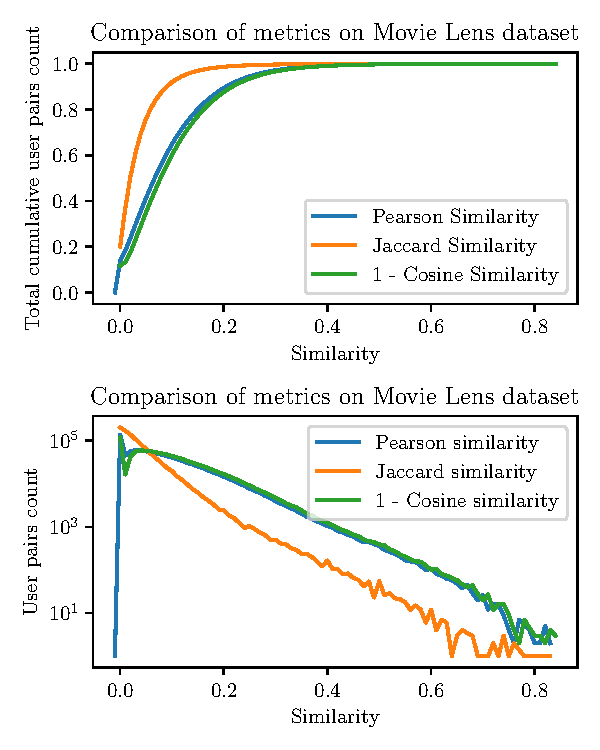
\includegraphics{img/figures/similarity_metrics.pdf}
    \caption{Comparison of similarity metrics on Movie Lens dataset.}
    \label{fig:similarity_metrics}
\end{figure}

% We have additionally considered Cosine similarity, but in our case it is important to consider only ratings that are a positive match due to most user item ratings not being present and therefore having value of '0'. The Cosine similarity would put users with sparse item ratings closer together due to taking matching 'zeros' as similar. The same hold for Jaccard similarity if we allow the intersection to match on 'zeros'.

We have compared the similarity metrics on a random sample of 1 million user pairs on \ref{fig:similarity_metrics}. Originally, we wanted to select Pearson Correlation Coefficient based on the before mentioned stability, but interestingly, PCC and the Cosine similarity are overlapping substantially. This is due to the ratings being very sparse which causes the means in PCC calculations to be close to 0 which then corresponds to the Cosine similarity. Further, PCC and Cosine similarity on average have more samples with higher similarity and less samples with lower similarity. We therefore select Cosine similarity as our similarity metric, due to its similarity to PCC and better properties than Jaccard similarity.

Now, we have a method of how to determine a similarity of two users. Further, we need to have a way of how to modulate the amount of similarity in the group. There is many interesting ways as how to create synthetic groups. Let us now present some of them.

Some of possible types of group creation:
\begin{itemize}
    \item \textbf{Random:}
        Randomly sample without replacement from the user-pool.
        
    \item \textbf{Similar:}
        Select one user randomly as a pivot, then fill in the remaining group spots with users that are as similar as possible. This basically is the k-nearest neighbours algorithm. Problem with this approach is that very rarely we encounter situations like this in the real world. Another problem is that selecting the most similar users is computationally expensive as we need to compute similarity between the pivot and every other user in the dataset. Which is not ideal for the sizes of our data.
        
    \item \textbf{Somehow similar, with outliers:}
        One other way how to relax the similarity is to randomly select a pivot user and then select the nearest neighbours only from a random subset of the whole user-pool. This way, we still get pretty similar users and do not need to perform so much computation.
        
        Other idea would be to select the next candidate based on the similarity to the last selected user instead of the pivot. In a way creating a chain of users based on the similarity of the individual links(users). This way, we could create more variable preference among the group members with still overlapping user-item interactions.
        
        Additionally, instead of selecting top-k similar users, we can make random steps in the similarity ordering, such as if we have 1000 most similar users ordered by the similarity metric, we do not need to take the top-k best ones, but for example 100th most similar, 200th most similar and so on.
        
        Further, instead of a top-k, we can select users based on a weighted probability generated either from the similarity or from the ordering of all the candidate members.
        
    \item \textbf{Similar to the whole group:}
        Instead of selecting candidates to be similar to a single main user, we can select next group members to incrementally be similar to group members already assigned, either by aggregating the ratings or by for example Borda count, this has the advantage of easier candidate selection, due to the bigger possible preference overlap. But it has a disadvantage of needing to perform more computation of similarity after each individual member selection.
        
    \item \textbf{Dissimilar:}
        Apart from finding group members based being as similar as possible, we can also try to create as dissimilar groups as possible. Here we can randomly select a first user and then select the next user which is as least similar as possible. Next, instead of selecting another user in the same way, we can calculate dissimilarity of all other uses with the joined preference of the users that are already selected to the group and again, select the most dissimilar one.
\end{itemize}


% -------------------------------------------------------------------------------------
\subsection{Selected approach}
% -------------------------------------------------------------------------------------
Let us now specify, in detail, the methods that we use and how we set the required parameters.

Easiest and most convenient option would be to calculate the similarity matrix for all users and then select groups based on this single calculation. But, this matrix can become pretty huge with the growing amount of users. Lets assume our worst case of 1,000,000 users of the Spotify dataset. Then we will have $10^{12}/2$ of similarity calculations that need to be processed and stored. This becomes difficult to manage as the amount of memory needed would be around on the order terabytes and the time needed for processing on the order of hours or days. We therefore opt for an iterative approach, where we randomly select only a smaller subset of potential group members and select the actual group members from this smaller group instead of the whole user pool. This can lead to calculating the users' similarity multiple times, but that that situation is somewhat unlikely and in total we will save orders of magnitude worth of similarity calculation (potentially depends on the number of groups we want to generate).

\subsubsection{At random}
Straightforward approach that generates groups with very distinct user preferences. We select the desired amount of users for one group from the user-pool and assign them together. Then repeat with the whole user-pool (not removing the selected members) again.

\subsubsection{Similar groups with top-k selection}
We select one user as a pivot of the group at random. Next we select some amount of users at random from the dataset as candidates and calculate the similarity between the pivot and each of the selected user candidates. Next we select the top-N most similar users to the pivot where N is the desired group size - 1 and fill in the rest of the group with these top-N most similar.

This ensures that there will be a pressure for similarity using the top-K mechanism as well as some variety due to the random selection of candidates.

\subsubsection{Similar groups with probability respecting similarity (PRS)}
We perform the same random selection as in the previous method for similar groups, but with a different procedure in the second step of selection from the candidates. We would like to select a candidate with a probability that corresponds to their similarity with the pivot user and decreases quite heavily to still ensure there is enough of a push towards selecting similar users.

\begin{figure}[ht!]
    \centering
    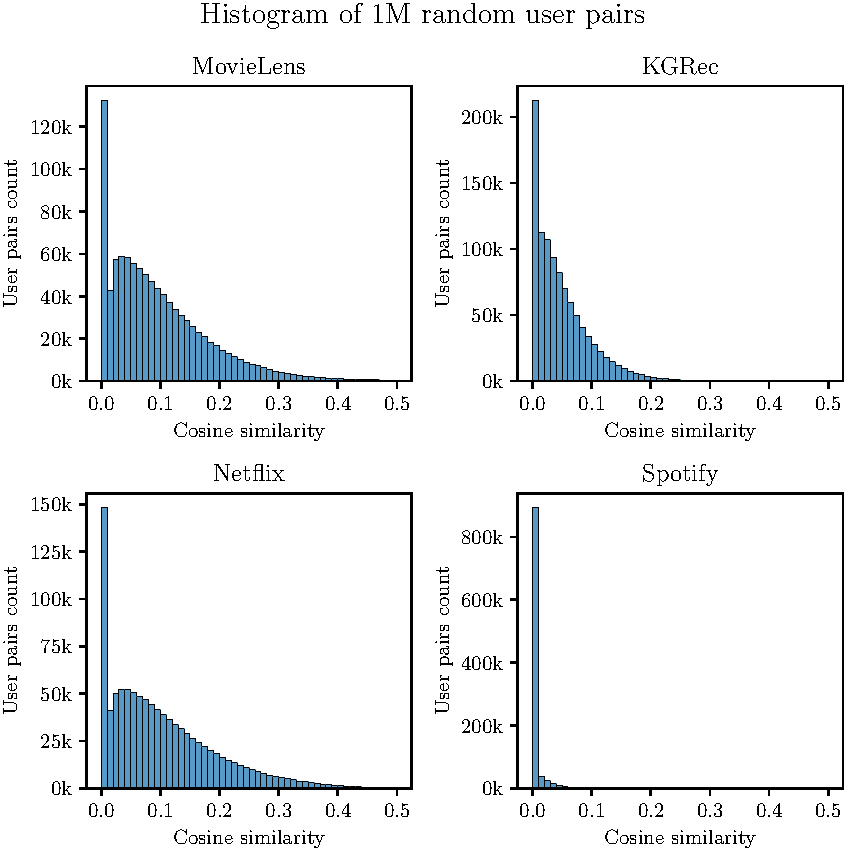
\includegraphics{img/figures/histogram_cosine_all.pdf}
    \caption{Histogram of cosine similarity of 1 million random user pairs from Movie Lens dataset.}
    \label{fig:cosine_all_histogram}
\end{figure}

Due to the exponentially decreasing number of users with higher similarity scores as can be seen on Figure \ref{fig:similarity_metrics} and in detail on Figure \ref{fig:cosine_all_histogram}, we need to ensure that potential group members with higher similarity still retain overall higher probability of being selected. We can do that by presetting the desired probability to the each cosine similarity group and then dividing this probability by the average number of user pairs in that similarity group.

Unfortunately, we do not have the precise average number of user pairs, which would require to compute similarity between all possible pairs. We can get a good estimation by sampling some amount of user pairs and calculating the ratio between the size of the group and the number of total samples. Sample of size 1 million on all datasets can be seen on Figure \ref{fig:cosine_all_histogram}.


In order to avoid deciding on the correct amount of bins to split the data into and how to smooth and sample from the bins, we have selected to model the expected cosine similarity probability density function minimizing the L2 norm. That allows us then to calculate what is the expected amount of samples in a small neighbourhood. For Movie Lens have selected an exponential distribution with parameter $\lambda=0.08918$. This distribution models our underlying data quite well, comparison can be found in Table \ref{table:5.3_modeled_comparison}. Most important portion of samples between 0.4 to 0.8 where most of the members with highest chance of being selected will fall, seems to be modeled quite precisely.
Then we can express the average expected amount of similarity pairs with similarity of $x$ in some small constant sized neighbourhood of size $NS$ to be:
\begin{equation}
    expectedSampleRatioOnInterval(x, N, \lambda) = cdf(exp(\lambda), x + N) - cdf(exp(\lambda), x),
\end{equation}
where cdf stands for the cumulative distribution function of in this case exponential distribution with the $\lambda$ parameter of $0.08918$.

\begin{table}[!ht]
    \centering
    \begin{tabular}{ c | c | c}
       cosine sim. & sampled data & $exp(\lambda=0.08918)$ \\
        \hline
        $\left[ 0.0, 0.1\right)$ & 600,716 & 674,139 \\
        $\left[ 0.1, 0.2\right)$ & 275,099 & 219,675 \\
        $\left[ 0.2, 0.3\right)$ & 90,355 & 71,583 \\
        $\left[ 0.3, 0.4\right)$ & 24,265 & 23,326 \\
        $\left[ 0.4, 0.5\right)$ & 6,660 & 7,601 \\
        $\left[ 0.5, 0.6\right)$ & 2,181 & 2,476 \\
        $\left[ 0.6, 0.7\right)$ & 602 & 807 \\
        $\left[ 0.7, 0.8\right)$ & 110 & 263 \\
        $\left[ 0.8, 0.9\right)$ & 12 & 85 \\
        $\left[ 0.9, 1.0\right]$ & 0 & 27 \\d
        total & 1,000,000 & 999,982
            
    \end{tabular}
    % \caption[Rating of selected GRS datasets.]{Rating of selected GRS datasets. Note for 'n/a' - we were unable to download the dataset, therefore unable to asses this criteria}
    \caption{Comparison of histograms of data sampled from the dataset and the created data model.}
    \label{table:5.3_modeled_comparison}
\end{table}

But we are not necessarily interested in the expected amount of samples on an interval, the main requirement is to have a ratio of expected occurrence between the sampled similarities. We are uninterested in the actual value, therefore approach using a probability density function of the modeled distribution is better. We can calculate the ration as follows:

\begin{equation}
    expectedSampleRatio(x, \lambda) = pdf(exp(\lambda), x) = \lambda e ^{-\lambda x},
\end{equation}
where pdf represents the probability density function.

Next, we need to have a way as how to scale the actual similarity. We would like to have a non-linear difference between samples. If a sample $A$ has similarity higher than sample $B$ by $0.1$, then we would like to have the sample $A$ to be selected twice as likely. Further, we can generalize the the difference as parameter $D$ and the multiplying factor as $M$.

We get:
\begin{equation}
    scale(x, D, M) = M^{\frac{1}{D}x} = M^{\frac{x}{D}},
\end{equation}
where for doubling the probability every 0.1 similarity difference will become:

\begin{equation}
    scale(x, 2, 0.1) = 2^{\frac{x}{0.1}} = 2^{10x}.
\end{equation}


\begin{equation}\label{eq:weight}
    \begin{aligned}
        weight(x, D, M, \lambda) &= \frac{scale(x, D, M)}{expectedSampleRatio(x, \lambda)} \\
        & = \frac{M^{\frac{x}{D}}}{\lambda e ^{-\lambda x}}
    \end{aligned}
\end{equation}

The parameter D in scale calculation has a big impact on the scaling, and unfortunately it needs to be tuned to each dataset separately due to the different ratings distributions as can be seen on Figure \ref{fig:cosine_all_histogram}. Through experimentation we have observed that the value of 0.1 seems to give us good results on every dataset apart for Spotify, where the width needs to be shortened substantially. We solve this situation by setting the parameter to the width of the interquartile range of the sampled ratings. In other words, we set it to the width of the middle 50\% mass for each dataset. We can see the resulting parameters for each dataset based on 1 million random user pairs in Table \ref{table:5.3_interquartile_width}. 

\begin{table}[!ht]
    \centering
    \begin{tabular}{ l l}
        dataset & \makecell[l]{interquartile \\ width (D)} \\
        \hline
        MovieLens & 0.104 \\
        KGRec & 0.057 \\
        Netflix & 0.114 \\
        Spotify & 0.025
            
    \end{tabular}
    % \caption[Rating of selected GRS datasets.]{Rating of selected GRS datasets. Note for 'n/a' - we were unable to download the dataset, therefore unable to asses this criteria}
    \caption{Scaling width parameter based on interquartile range of each dataset.}
    \label{table:5.3_interquartile_width}
\end{table}



\begin{algorithm}
	\caption{Generate groups with probability respecting similarity}
	\begin{algorithmic}[1]
	    \State Select scaling parameter $M$ and the desired amount of samples $S$ and amount of candidates $C$
	
	    \vspace{3mm}
	
	    \For {Desired number of samples $S$}
    	    \State Select random pair for users $u1$ and $u2$ from the user-pool
    	    \State Calculate similarity of $u1$ and $u2$ and store it
	    \EndFor
	    \State Fit an exponential distribution to the stored values
	    \State Calculate the width between 25th and 75th quartile as parameter D
	    \State Get its parameter $\lambda$
	    
	    \vspace{3mm}
	    
	    \For {Number of desired groups}
    	    \State Select 1 user $uCaptain$ from the user-pool as main user
    	    \State Select $C$ random users as $uCandidates$ from the user-pool
    	    \For {Each user $u$ from $uCandidates$}
    	        \State Calculate similarity between $uCaptain$ and $u$ as $sim$
    	        \State Calculate random candidate weight with (Eq. 5.8):
    	        \State $weight$ = scale($sim$, D, M) / expectedSampleRatio($sim$, $\lambda$)
    	    \EndFor
    	    \For{ Desired group size - 1}
    	    \State Perform weighted random selection on the candidates using the weights
    	    \State Add the selected user to the group and remove it from the candidates
    	    \EndFor
        \EndFor
	\end{algorithmic}
	\label{alg:create_sim_groups}
\end{algorithm} 



This gives us a framework as how to assign each candidate member a weight by which we can perform a weighted random choice and therefore introduce more variability into the group selection process. The full equation for a sample's weight can be calculated with equation \ref{eq:weight}, further, we describe the whole group generation process in Algorithm \ref{alg:create_sim_groups}.










% Pearson Correlation Coefficient due to its stable performance as mentioned in \cite{similarity_measures_comparason},  and due to its wide use among the recommender system domain.

% \textbf{Pearson correlation coefficient} for two vectors $X$ and $Y$ can be computed as follows:
% \begin{equation}
%     P(X,Y) = \frac{\text{cov}(X,Y)}{\sigma_x \sigma_y}
%     = \frac{{}\sum_{i=1}^{n} (x_i - \overline{x})(y_i - \overline{y})}{\sqrt{\sum_{i=1}^{n} (x_i - \overline{x})^2(y_i - \overline{y})^2}},
% \end{equation}
% where $cov$ is the covariance, and $\sigma$ is the standard deviation.

% Further we have selected \textbf{Jaccard similarity} due to its simplicity:
% \begin{equation}
%     J(X,Y) = \frac{|X \cap Y|}{|X \cup Y|} = \frac{|X \cap Y|}{|X| + |Y| - |X \cap Y|}.
% \end{equation}
% It has a 

% -------------------------------------------------------------------------------------
\subsection{Evaluation of the generated groups}
% -------------------------------------------------------------------------------------

% TODO: We want to evaluate the selected methods
% first, select how to measure,
% present our measurement graficek

We have implemented and used the selected techniques to generate synthetic groups. Let us now evaluate the performance of each method. And discuss the parameters of the generation process.

The random method is the simplest from the point of selecting parameters of the group creation. It does not have any.

Next, the top-k method, it only has a single parameter of the number of candidates from which we choose the actual group members. We have set the default number of candidates to 1000, due to the computational complexity rising linearly with the amount of candidates.

And lastly, the our PRS method. It has 3 parameters in total, where $\lambda$ is parameter of the exponential distribution fitted to a sample of user similarities. D is the distance and M the multiplier factor of the scale ratio. We have set the distance to be 0.1 and we vary the multiplier factor from 0,5 to 4.

We aim to compare the mean inter-group similarity. First, we define subset of size $n$ of set $S$ as

\begin{equation}
    R(S, n) := { x \in \mathcal{P}(S) : |x| = n},
    \end{equation}
where $\mathcal{P}$ is a powerset, set of all subsets. 

Then we define the inter-group similarity which represents the mean of similarity between all tuples in the group as
\begin{equation}
    intergroupSimilarity(G) = \frac{1}{|R(G,2)|}\mathlarger{\sum}_{\{a,b\} \in R(G,2)}  cos(a,b).
\end{equation}


\begin{figure}[ht!]
    \centering
    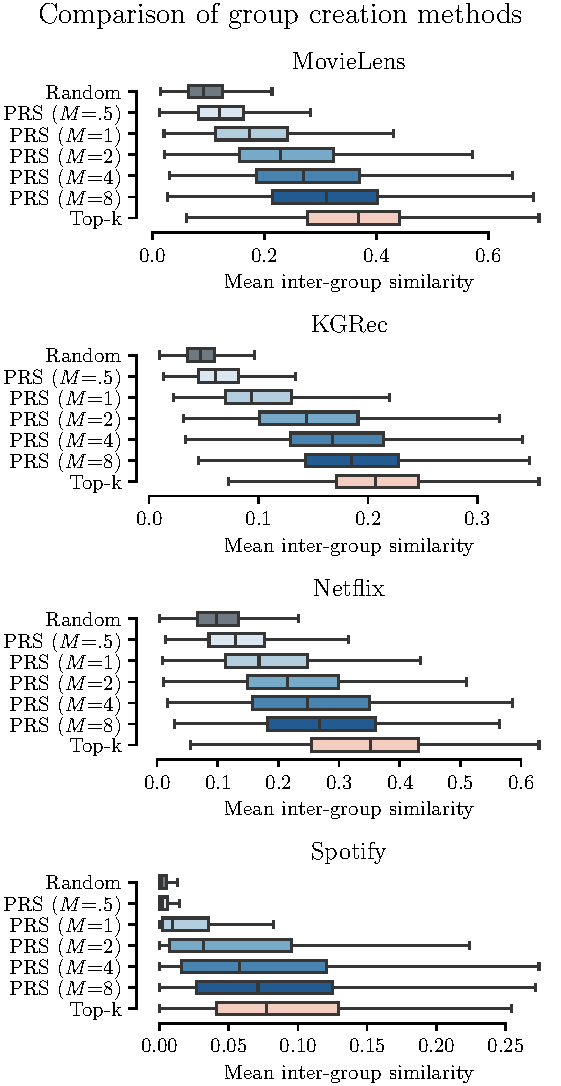
\includegraphics{img/figures/inter_group_means.pdf}
    \caption[Comparison of Random, Top-k and multiple variants of PRS group generation of size 5.]{Comparison of Random, Top-k and multiple variants of PRS group generation for groups of size 5. Number of candidates for PRS and Top-k was 1000.}
    \label{fig:inter_group_means}
\end{figure}

With each group generation method we have created 1000 groups of size 5. The resulting mean inter-group similarities can be seen on Figure \ref{fig:inter_group_means}. As expected, the random and top-k have the least and most mean inter-group similarity. With PRS we have achieved the desired scaling of the mean inter-group similarity between the random and top-k. Further more, we see that PRS generates groups that are comparably or more varied in the similarity as top-k, this is important. Other methods, which manage to create groups that utilize some sort of similarity scaling such as in \cite{GFAR-kaya2020} that select candidates based on their similarity with the pivot will not produce groups that vary in the inter-group similarity.

At first PRS did not scale well on the Spotify dataset with parameter D set to 0.1. The dataset has its similarity concentrated closer to zero. The reason for this is that most users (playlists) did rate not more than 30 items. Majority ratings are between $0$ and $0.1$, we therefore need to set the scaling width to a lower value in order to compensate for this. Based on this we have introduced the technique of setting the D parameter to the width of the interquartile range which solves the issue and decreases the amount of parameters that need to be tuned to only one - the scaling parameter M. 

In conclusion, we are satisfied with the PRS technique. It provides us with a method how reliably generate groups of varying inter-group similarity which are more heterogenous and therefore closer to reality than selecting group members directly based on the desired similarity.

\section{Dataset tool} \label{sec:dataset_tool}

We have created a Python CLI tool that allows users to download and process datasets mentioned in \ref{sec:single_user_datasets} and create artificial groups with methods described in \ref{sec:creation_of_artificial_groups}.

\todo[inline]{add parameters, screenshot and requrements}

% - clanky co cituji gfar vytvarely umele skupiny, prozkoumat,
% - lada clanek jednotlive popisy
% - porovnani prozkoumani a nasledne shrnuti/vylepseni

\chapter{Proposed group recommender system}  \label{chap:our_work}

As we have discussed so far, group recommendation is not an easy task. There are many social and mathematical optimization criteria that are hard to define and even harder to measure. Let us now present our algorithm that aims to provide group recommendations that optimize fairness and relevance. We published this algorithm originally at UMAP'21 in \cite{our_ep_fuzz_da}.

\section{Preliminary}

In our context, we see fairness as a property that no user should be systematically discriminated against when it comes to their satisfaction with the recommended items. Optimizing this type of fairness is hard, especially when we have a user or a subset of the group whose preferences differ from the rest.

Some algorithms, such as the Average (AVG) and Least Misery(LM), already optimize for fairness (even if not primarily designed for that purpose). We can say that AVG strategy is fair due to its property that it considers all members' preferences as equally important. If the task is to recommend only a single item, then there is not much improvement to be made apart from how we define what we consider fair. However, that is different for tasks where we recommend a list of items or we have multiple following recommendation sessions. Then we can tweak our following recommendations to fix our previously introduced fairness imbalance.

Let us now classify approaches by how they optimize fairness into the following groups: \textit{item-wise}, \textit{list-wise}, and \textit{rank-sensitive} fairness.

Firstly, item-wise approaches optimize single-item performance. They usually apply some form of aggregation, such as average for the AVG or minimum for the LM approach. Scores for each item are calculated independently, and so scores for one item do not affect scores for any other.

Secondly, \textit{list-wise} approaches take into consideration which items have been recommended before. This allows us to balance fairness among group members over multiple consecutively recommended items. All before mentioned methods from Subsection \ref{subsec:specific_cases_of_fairness} fall into this category. In other words, items are not recommended independently, but the total fairness of items recommended in succession is important. The simplest example of a \textit{list-wise fairness} approach is FAI. We select for each user, in turn, their most preferred item. This way, at some point, each user will be satisfied, and FAI therefore indirectly balances the per-user utility.

We can define a per-user utility function $r_u; u \in G$, which measures the specified properties that we aim to optimize during the process of generating a list of recommended items. We can then use this utility function to control the recommendation of the following items to balance fairness among the group members. Most commonly, the utility function is a mean of predicted relevance for each user.

Moreover, lastly, \textit{rank-sensitive} approaches optimize fairness for each prefix of the recommended list of items. This approach has theoretically ideal properties in use cases where we do not know what portion of the recommended list will be consumed or viewed by the users. We only know about a single related approach from this category, GFAR \cite{GFAR-kaya2020}. As already described in Subsection \ref{subsec:03_advanced_methods.gfar}, the authors define fairness through the sum of probabilities that at least one item from the list will be relevant to each user.

Our proposed algorithm falls into the group of \textit{rank-sensitive} approaches. It maximizes the per-user proportional fraction of total relevance. Compared to GFAR, it does not define fairness based on the ranks of items. This gives it more freedom in the item selection process due to rank sensitive approach discounting the relevance of items with decreasing rank quite quickly, even if, in reality, items on lower ranks can still present a great option.

As already mentioned in our paper about this algorithm \cite{our_ep_fuzz_da}, the main inspiration for our work is election algorithms that are used for mandates allocation.
Mandate allocation is an important problem in distributing mandates based on the votes received. The important part of the problem is what to do if the votes are not divisible in the way that would allow to distribute them by a simple one mandate per a set number of votes without any remaining votes left unassigned.

We focus on D'Hondt's algorithm (DA). It, as already stated in Subsection \ref{subsec:03_advanced_methods.DHondtDO}, is commonly used in election systems around the world. It is a greedy selection algorithm that minimizes the number of votes that need to be left aside so that the remaining votes are represented exactly proportionally as described in \cite{wiki:dhondt_method}.

D'Hondt's algorithm procedure works in discrete steps, where in each step, it selects the party with the maximum quotient $quot$ one seat. The quotient for each party is calculated as the total number of votes the party has received $V_p$ divided by the number of seats $s_p$ + 1 that has already been awarded to that party $p$. Initially, $s_p$ is set to zero.

\begin{equation}
    quot(V_p, s_p) = \dfrac{V_p}{s_p + 1},
\end{equation}

Directly using the DA algorithm is not possible due to it being designed for discrete mandate allocation problems. But this unfortunate property has been addressed in \cite{fuzz_da}. We describe the method of D'Hondt's direct optimization in more detail in Subsection \ref{subsec:03_advanced_methods.DHondtDO}.

\section{EP-FuzzDA}

Let us now describe our algorithm of \textbf{E}xactly \textbf{P}roportional \textbf{F}uzzy \textbf{D}'Hondt's \textbf{A}ggregation. It is a greedy algorithm that iteratively selects the best candidate item maximizing the marginal gains on \textbf{E}xactly-\textbf{P}roportional \textbf{rel}evance \textbf{sum} (EP-rel-sum) criterion.

As mentioned before, candidate allocation algorithm such as D'Hondt does not consider the varying relevance of candidate items nor the possible overlap of user preferences. Both these situations are very common in the domain of group recommender systems. We can probably find a set of items that closely balance the relevance between all group members. Nevertheless, each of these items may have a different candidate item that is a better fit for the group in the average rating but would lead to more imbalance. This could easily lead to recommending mediocre items only for the sake of balancing fairness.

We, therefore, want to maximize the balance of items' utility for each group member but without hindering the possible additional utility provided to members that overlap in preference with other members or are easier to satisfy. One solution is to optimize for the total item relevance but cap the maximum possible gain for each individual user so that it does not further add to the total item score. We call this cap \textit{exactly proportional relevance allowance}. It is calculated as a proportional share of each user on the total sum of all so far selected items' relevance.


Let us assume that we have already selected items $\mathcal{L}$ (this set can be empty), with individual relevance of $r_{i,u}$ for all items $i \in I$ and users $u$ of a group $\mathcal{G}$. We will use the example in Table \ref{table:6.2_relevance_example} for the following calculations.

\begin{table}[!ht]
    \centering
    \begin{tabular}{c | c c c | c c c c}
               &       &       &       &      &    & \multicolumn{2}{c}{EP-FuzzDA} \\
        Object & $u_1$ & $u_2$ & $u_3$ & AVG  & LM & step 1 & step 2\\
        \hline
        $c_1$ & 0.9 & 0.8 & 0.0 & 0.567 & 0.0 & 1.13 & - \\
        $c_2$ & 0.6 & 0.5 & 0.0 & 0.367 & 0.0 & 0.73 & 0.17 \\
        $c_3$ & 0.5 & 0.9 & 0.0 & 0.467 & 0.0 & 0.93 & 0.37 \\
        $c_4$ & 0.0 & 0.1 & 0.9 & 0.333 & 0.0 & 0.43 & 1.00 \\
        $c_5$ & 0.1 & 0.1 & 0.8 & 0.333 & 0.1 & 0.53 & 0.90 \\
        $c_6$ & 0.2 & 0.0 & 0.7 & 0.300 & 0.2 & 0.50  & 0.70 \\
    \end{tabular}
    \caption[Example of relevance calculation for item-wise aggregations]{Example of relevance calculation for item-wise aggregations. Least-misery, average, and two steps of our DA method. Step 2 is after selecting $c_1$ in step 1.}
    \label{table:6.2_relevance_example}
\end{table}


We then calculate the relevance allowance for a new candidate item as follows. First, we sum up relevance for all users for all already selected items as 
\begin{equation}
    TOT(\mathcal{G}, \mathcal{L}) = \sum_{i \in \mathcal{L}}\sum_{u\in \mathcal{G}} r_{i,u},
\end{equation}

Then we define $TOT_c$ for a candidate item $c$ (different from all already selected) as $TOT(\mathcal{G}, \mathcal{L} \cup c)$. This represents the prospected total utility if we would select the candidate $c$.




We then calculate the maximum allowed utility (relevance) with the appropriate weight of a user $w_u$ as:
\begin{equation}
    allowed\_utility_u = TOT_c * w_u.
\end{equation}

The weight of each group member can either be set to $1/|\mathcal{G}|$ or arbitrarily so that $\sum_{u \in \mathcal{G}} w_u = 1$. This weight represents how important each user is in the group and will scale the preferred utility ratio between group members if not set uniformly.

In our example in Table \ref{table:6.2_relevance_example}, at step 1. we have $TOT_{c1} = 0.9 + 0.8 + 0.0 = 1.7$ which scaled by uniform weight of $1/3$ to $ 1.7 * (1/3) = 0.57 = allowed\_utility_u$. We then calculate the unfulfilled relevance as the total received utility (from already selected items in $\mathcal{L}$) subtracted from the maximum allowed utility. We are selecting the first item. Therefore all users start with a received utility of 0, which makes the unfulfilled relevance for candidate item $c_1$ set to $0.57$ for all users.

\begin{equation}\label{eq:list_user_relevance}
    \mathit{total\_received\_utility}_u= \sum_{i \in \mathcal{L}} r_{u,i},
\end{equation}

\begin{equation}
    \mathit{unfulfilled\_rel}_u= max(0, allowed\_utility_u - \mathit{total\_received_utility}_u).
\end{equation}

We can then finally calculate the utility of each item by
\begin{equation}
    \mathit{rel}_i= \sum_{u \in \mathcal{G}} min(rel_{u,i}, \mathit{unfulfilled\_rel}_u).
\end{equation}


We can now calculate the utility of item $c1$ as $min(0.9, 0.57) + min(0.8, 0.57) + min(0.9, 0.57) = 1.13$. And similarly for all other candidate items. After the first round, we select $c1$ and follow into a second one. Now it starts to get interesting because we need to calculate the total received utility and use it to calculate the unfulfilled relevance correctly.

For item $c_2$ we have $TOT_{c_2} = 1.7 + 0.6 + 0.5 + 0.0 = 2.8$ (1.7 is $TOT$) and user $u_1$ we have unfulfilled relevance of $2.8 / 3 - 0.6 = 0.03$, for user $u_2$ we have $2.8 / 3 - 0.8 = 0.13$ and for $u_3$ we have $2.8 / 3 - 0.0 = 0.93$. All numbers are capped to the min 0. So in total the relevance of item $c_1$ is $min(0.6, 0.03) + min(0.5, 0.13) + min(0.93, 0.0) = 0.16$. We can see the output of relevance calculations for all items in the example table under column step 2. In the second step, we would therefore select item $c_4$.

Let us now be more formal with the definition of EP-rel-sum. We have a list of recommendations $\mathcal{L}$ and its total relevance $TOT$ as defined previously. Next, we have the $r_u$ total relevance of all items from $\mathcal{L}$ for user $u$ as defined with Equation \ref{eq:list_user_relevance}. Further, we have the per-user proportional relevance allowance $a_u$ ($\mathit{allowed\_utility_u}$)  as $TOT * w_u$. Weights $\sum_{u \in \mathcal{G}} w_u = 1$. 
Then we finally define the EP-rel-sum criterion as

\begin{equation}
    \textrm{EP-rel-sum}(\mathcal{L}_G) = \sum_{\forall u \in \mathcal{G}} \min(r_u, a_u).
\end{equation}

We can observe that for two lists $L_G^1$ and $L_G^2$ with the same total relevance, EP-rel-sum will be higher for the list more proportional to the weights $w_u$ distribution. Another way around, if we have two lists with the same relevance distribution, the one with higher total relevance will receive a higher EP-rel-sum score.

\begin{algorithm}\label{alg:fuzzy_dhondt}
    \caption{Exactly-Proportional Fuzzy D'Hondt's Aggregation}
    \begin{algorithmic}[1]
        \State {\bfseries Input:} group members $u \in \mathcal{G}$, candidate items $i \in \mathcal{I}$, relevance scores $r_{u,i} \in \mathbf{R}$, \#items to recommend $k$, user's weights $w_u$; $\sum w_u = 1$ 
        \State {\bfseries Output:} ordered list of group recommendations $\mathcal{L}_G$ of size $k$
        \vspace{1mm}
        \State $\mathcal{L}_G = []$ 
        \State $TOT = 0$
        \State $\forall u: r_u = 0$
        \vspace{1mm}
        \For{$1$ to $k$}
            \For{$i \in \mathcal{I} \setminus \mathcal{L}_G$}
                \State $TOT_c = TOT + \sum_{\forall u} r_{u,i}$
                \State $\forall u: \mathit{allowed\_utility}_u = TOT_i * w_u$
                \State $\forall u: \mathit{unfulfilled\_relevance}_u = max(0, \mathit{allowed\_utility}_u - r_u)$
                \State $gain_i = \sum_{\forall u} min(r_{u,i}, \mathit{unfulfilled\_relevance}_u)$
            \EndFor
            \State $i_{best} = \argmax_{\forall i}(gain_i)$
            \State append $c_{best}$ to $\mathcal{L}_G$
            \State  $\forall u: r_u = r_u + r_{u,i_{best}}$
            \State $TOT = \sum_{\forall u} r_u$
        \EndFor
        \State \textbf{return} $\mathcal{L}_G$ 
    \end{algorithmic}
\end{algorithm}

And finally, to make EP-rel-sum ranking sensitive, as previously described, we define marginal gains while extending the list of items as

\begin{equation}
    gain(\mathcal{L}_G, c_j) = \textrm{EP-rel-sum}(\mathcal{L}_G \cup \{c_j\}) - \textrm{EP-rel-sum}(\mathcal{L}_G).
\end{equation}

EP-FuzzDA, which we describe in Algorithm \ref{alg:fuzzy_dhondt}, iteratively selects the item that provides the maximal marginal gain to the already selected set of items. It, therefore, is a \textit{rank-sensitive} approach for optimizing fairness.

Another nice property not present in other group recommendation algorithms is that our algorithm naturally incorporates scaling of user preference importance using the weights $w_u$. We will use this later in our experiments for weighted groups and long-term fairness evaluation.

% -------------------------------------------------------------------------------------
\chapter{Experiments}  \label{chap:experiments}
% -------------------------------------------------------------------------------------

Let us now talk about our experiments. First, we describe the evaluation process, which we use, and the rationale behind it. Then, we present the data flow and software we have written, and finally, we present the results.

The following experiments are an extension of our original research paper \cite{our_ep_fuzz_da}. Differences and extensions that have been made will be discussed further. Most notably, they are the addition of 3 new datasets, different matrix factorization algorithms, and a different group generation method.


All code for Python scripts and Jupyter notebooks can be found at \newline\href{https://github.com/LadislavMalecek/MasterThesisAnalysis}{github.com/LadislavMalecek/MasterThesisAnalysis}. All file paths mentioned in this chapter assume to have the base path at the root of this repository (when cloned on the disk).

% -------------------------------------------------------------------------------------
\section{Evaluation}\label{subsec:experiments.evaluation}
% -------------------------------------------------------------------------------------

Our experiments are run in an offline setting. We therefore only have the users' preferences, not the actual group ratings. Further, as discussed in Chapter \ref{chap:datasets}, we do not have a dataset that would contain group preferences, nor a dataset that would contain any group information. Let us now discuss the separate parts of the evaluation and the choices we have made in the experiments. Later we will put everything together and go through each step of the experiment.

% -------------------------------------------------------------------------------------
\subsection{Coupled vs. decoupled} \label{subsec:07_experiments.evaluation.coupled_decoupled}
% -------------------------------------------------------------------------------------
One of the problems with group recommendation systems is the evaluation. In the case of a single-user RS, it is common to have the data split into training, validation, and testing parts. This way, for example, if we train a matrix factorization algorithm, we can check how it is performing at the end of our training using the testing portion of the dataset which is separated from the data that has been used for training.
This can be used even if the user ratings are very sparse, which in the majority of cases they are. But with multiple users, such is the case for group RS, we would need to have the ratings overlapping for the group members, meaning that they all have rated the same items. Even worse, with each additional member, the overlap of ratings will become smaller and smaller.

We can distinguish between two main approaches for evaluating group recommendation systems - coupled and decoupled.

The main difference, as we can see in Figure \ref{fig:coupled_decoupled}, is that in the \textbf{coupled} (tightly coupled with the underlying RS) evaluation approach, we evaluate our performance on a with-held set of testing data and in the \textbf{decoupled} evaluation, we consider the underlying single user recommendation system the source of our ground truth. The coupled approach, therefore, evaluates not only the group RS aggregation method but the underlying single-user RS as well.

The coupled evaluation has the undesired property of favoring group RS that tends to select the per-user best items as we have mentioned in \cite{peska2021coupled}.

\begin{figure}[ht!]
    \centering
    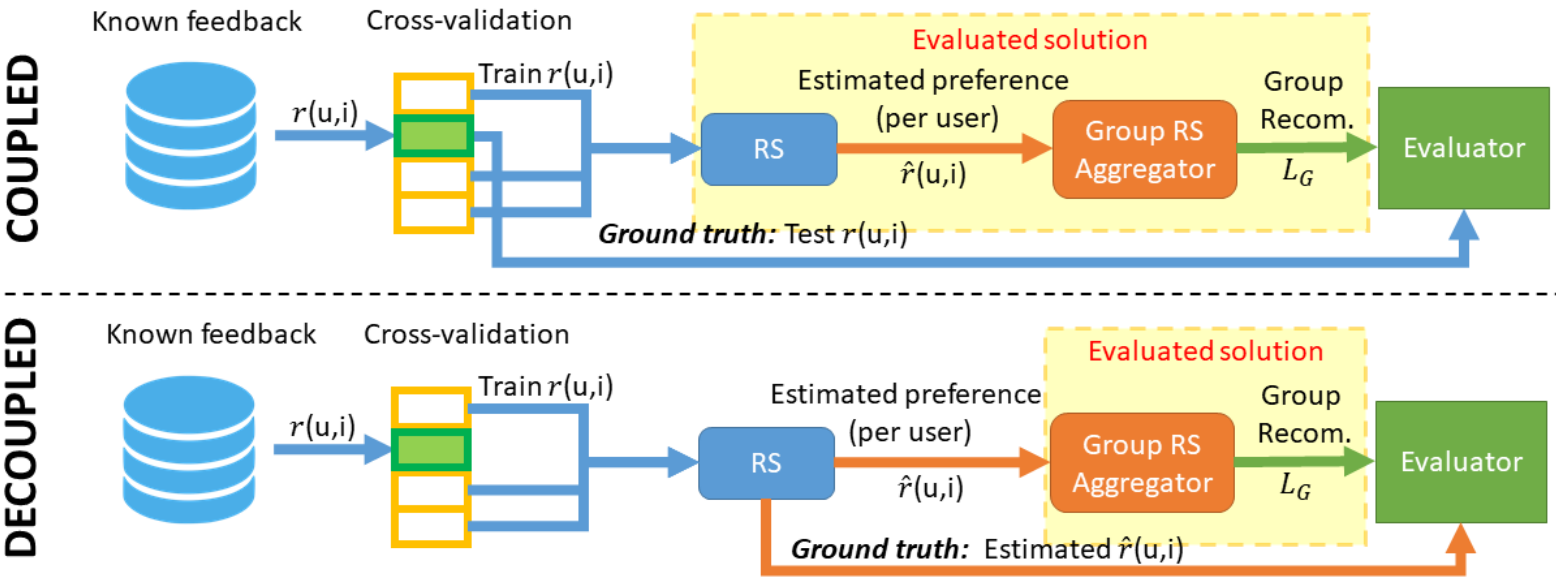
\includegraphics[width=5.5in]{img/coupled_decoupled_evaluation.png}
    \caption{Example of two main evaluation approaches from \cite{peska2021coupled}.}
    \label{fig:coupled_decoupled}
\end{figure}

% -------------------------------------------------------------------------------------
\subsection{Metrics}\label{subsec:07_experiments.evaluation.metrics}
% -------------------------------------------------------------------------------------

After running the group recommendation algorithm, we end up with a list of recommendations for each group. We now need to evaluate the performance of each algorithm.
For each group size, group type, and algorithm, we want to get a measure of how well they have performed.

Firstly, we need to get the ground truth from our underlying RS for each item and each group member.
Now for each group member and list of recommendations, we evaluate two metrics: normalized discounted cumulative gain (\textbf{nDCG}) and average relevance score (\textbf{AR}). We have chosen nDCG due to its popular use in our domain and a good representation of the probability of selection of an item based on the item's position in the list. AR metric has been chosen due to its simplicity and an overall good measure of performance for short lists of recommendations.

For each group and each user, we have \textbf{AR} and \textbf{nDCG} scores. Further, we calculate the aggregated per-group statistics for both of these metrics. We calculate \textbf{mean}, minimal user's score (\textbf{min}), and the ratio between minimal and maximal scores (\textbf{M/M}). All of these are valid fairness definitions on their own, depending on the definition of fairness as discussed in Chapter \ref{chap:fairness}. These metrics are also used in related literature \cite{GFAR-kaya2020}, \cite{sacharidis_2019_top_n_with_fairness}. Finally, we aggregate results for all groups together by calculating the mean of the metrics.

% -------------------------------------------------------------------------------------
\subsection{Evaluation use-cases}\label{subsec:07_experiments.evaluation.use_cases}
% -------------------------------------------------------------------------------------

In \cite{GFAR-kaya2020}, they focus only on the scenario of uniform groups, where each user is weighted uniformly. For our experiments, we are evaluating not only the \textbf{uniform} scenario but \textbf{weighted} and \textbf{long-term} scenarios as well.

In the \textbf{weighted scenario}, we randomly assign a weight to each of the group members (all summing up to a total of 1). This weight represents the non-uniform importance of each group member. This scenario is a relevant strategy for situations in structured groups where some members have a priority, such as a family with children watching a movie or a birthday party. This is an extension of the most respected person strategy described in \cite{most_respected_person}, with less rigid rules of only requiring weights to be in an interval of [0,1], with the total sum of weights in the group equal to 1.

In the \textbf{long-term scenario}, we assume that, in reality, the groups are more permanent with multiple instances of recommendation that are time separated. Such as a group of friends watching a movie every week or any other fixed group that consumes content together repeatedly. In this scenario, we want to prevent a systematic bias against one or multiple members and recommend items in the subsequent sessions with respect to the satisfaction and fairness of the previous sessions. We use the weights as in the previous weighted scenario and adjust them accordingly to satisfy the under-represented uses. We define the weights as a non-negative difference between the exactly proportional share of total relevance and the sum of relevance scores that the user has gained so far.

To evaluate the long-term scenario, we recommend items five times in a row, where after each row we calculate the appropriate weights and exclude the previously recommended items from further recommendation. After these five recommendation rows, we evaluate the mean utility for each user.


% -------------------------------------------------------------------------------------
\section{Evaluation setup} \label{sec:07_experiments.evaluation_setup}
% -------------------------------------------------------------------------------------
The experimental setup is an extended version from our \cite{our_ep_fuzz_da}. In the paper, we have used experiments from \cite{GFAR-kaya2020}, that we have extended with our algorithms and weighted and long-term recommendations.

Unfortunately, the original code from \cite{GFAR-kaya2020} we have worked with is quite proprietary and written in Java. For this work, we would have to extend it even further (compared to our work in \cite{our_ep_fuzz_da}) by adding the new group generation process that we have designed in Section \ref{sec:creation_of_artificial_groups}, new datasets, and a new matrix factorization. For convenience and further future research reusability, we have therefore made a decision to write all parts of the experiment in Python.

The main notable change from \cite{GFAR-kaya2020} is that we have modified the evaluation procedure. We use the decoupled evaluation instead of the coupled one as it gives an unfair advantage to algorithms that select the per-user best items and does not evaluate the underlying single-user RS in a coupled way as mentioned in Subsection \ref{subsec:07_experiments.evaluation.coupled_decoupled}.

Our experiments have 5 following steps.

% \begin{itemize}
    % \item \textbf{Data retrieval and processing:}
    \subsection{Data retrieval and processing}
        Unfortunately, as discussed in detail in Chapter \ref{chap:datasets}, we cannot host or append the used datasets directly to our code repository due to licensing. We have to therefore start with retrieving and processing the datasets.
        
        Run \path{./gather_datasets/downlad_and_transform.py} script directly if \newline you wish to retrieve the datasets manually. It supports Movie Lens, Netflix, KGrec, and Spotify datasets and performs cleanup and transformation to make further processing of the datasets as convenient as possible.

        The cleaning process transforms the datasets to a unified format with a single table of user ids, item ids, and ratings (if provided), normalizes and removes empty gaps from user and item ids, and validates the downloaded data.
    
        We have committed the weights that are outputted from the next step of matrix factorization to the repository. Therefore it is possible to skip this step if desired.

        
        
    % \item \textbf{Training matrix factorization algorithm:}
    \subsection{Training matrix factorization algorithm}
        We use two matrix factorization (MF) methods to generate our ground truths for the decoupled evaluation. First is our custom implementation of the highly parallel alternating least squares method (ALS) that we use for datasets with explicit ratings. The second is an implicit variation of the ALS method from a Python library Implicit \footnote{https://github.com/benfred/implicit} that we use for datasets with implicit ratings.

        As an output of this step, we get the two factors of MF, user and item factor matrix. We avoid saving the full target matrix due to the substantial size of the larger datasets, which would further increase our memory requirements. Instead, we calculate the ratings on the fly in the next steps.

        Run \path{./matrix_factorization/matrix_factorization.py} if you wish to calculate the matrix factorization manually.

        In our experiments, we use the following parameters for matrix factorization: number of iterations 15, random seed 42, regularization factor of 0.1, convergence threshold of 0.0001, and number of factors 50 for KGRec, 200 for Movie Lens, and 300 for Netflix and Spotify datasets. For KGRec and MovieLens datasets, we have selected the parameters similarly as in \cite{GFAR-kaya2020}. For other datasets, Netflix and Spotify, we have selected the parameters by hand based on a simple heuristic - the bigger and more complex the dataset, the higher the number of factors.
        
        Matrix factorization methods tend to degenerate when selecting the wrong parameters for the size of the factors, but the results for different types of groups (based on similarity PRS(M=1) and PRS(M=4)) do suggest that this is not the case, due to better results for groups with higher similarity (groups of more similar members are easier to satisfy). If the factors would degenerate and provide us only with flat ratings, then there would not be a difference in results for the two mentioned types of groups.

        We have committed the generated weights for all datasets into the code repository. Therefore it is possible to skip this step if desired. They are stored in a binary Numpy format with one exception for the Spotify dataset for which the item factor has reached the limit of GitHub LFS maximum file size. Therefore, we have zipped this dataset's factorization data in a standard .zip format.
        
    % \item \textbf{Creation of synthetic user groups:}
    \subsection{Creation of synthetic user groups}
        We have implemented 3 group creation strategies as already discussed in Section \ref{sec:creation_of_artificial_groups}. These are Random, Top-K, and Probability respecting similarity (PRS) algorithms. As shown in Figure \ref{fig:inter_group_means}, our method PRS nicely scales between the two extremes of Random and Top-K selection. We further assume that these two extremes do not often appear in real-world scenarios. Therefore, we have omitted them from our evaluation to simplify our experiments and only use groups created by the PRS algorithm.

        Run \path{./create_groups/create_random_groups.py} to create random groups \newline
        or run \path{./create_groups/create_topk_groups.py} to create Top-K groups \newline
        or run \path{./create_groups/create_prs_groups.py} if you wish to create PRS groups.
        
        We use PRS with two different settings of M, first at $M=1$ and second at $M=4$. Based on our analysis in \ref{subsec:04_creation_of_artificial_groups.evaluation}, we believe these two variants nicely represent the usual group setting.
        
        Further, for each setting, we generate 1000 groups in sizes 2, 3, 4, 6, and 8. We use 1000 candidates for each group, and lastly, we use 10,000 samples to get the dataset's similarity distribution.

        For weighted experiments, we additionally generate group weights as described in Subsection \ref{subsec:07_experiments.evaluation.use_cases}.
        
        Run \path{./create_groups/create_group_weights.py} if you wish to generate them manually.
    
    % \item \textbf{Running GRS algorithms:}
    \subsection{Running GRS algorithms}
        After the previous steps, we finally have all the required data to run GRS algorithm. We use the following algorithms from Chapter \ref{chap:related_work}: \textbf{AVG}, \textbf{LM}, \textbf{FAI}, \textbf{XPO\cite{sacharidis_2019_top_n_with_fairness}}, \textbf{NPO}, \textbf{GFAR\cite{GFAR-kaya2020}} together with \textbf{EP-FuzzDA} and is direct optimization variant \textbf{DHondtDO}.

        We use a computation optimization for all algorithms, where for each group member, we select their top 1000 candidate items (by rating), and then we compute the algorithm's item selection only on a joined set of these top items. Note that it is 1000 for each group member, so the number of candidate items in the set for the whole group will be bigger. For XPO and NPO, we use 30 candidate items instead of 1000 due to the computational complexity of those algorithms (this will be further discussed in \ref{sec:experiments.discussion}).

        Complete overview of all parameters for each algorithm:
        \begin{itemize}
            \item \textbf{AVG, LM, FAI}: candidate items = 1000
            \item \textbf{XPO, NPO}: candidate items = 30, monte Carlo trials = 100
            \item \textbf{GFAR}: candidate items = 1000, max relevant items = 100
            \item \textbf{EP-FuzzDA, DHondtDO}: candidate items = 1000, 
        \end{itemize}

        For each group and each algorithm, we get the top 10 items.

        Run \path{./experiments/run_algorithms.py},
        \newline
        \path{./experiments/run_weighted_algorithms.py} and
        \newline
        \path{./experiments/run_longterm_algorithms.py} to generate uniform, weighted and long-term experiments, respectively.
    
    % \item \textbf{Evaluation:}
    \subsection{Evaluation}
        The last step is an evaluation of the results. We have 4 datasets, 5 group sizes of 2, 3, 4, 6, 8. 2 types of groups, and 8 GRS algorithms. and 6 metrics combination as described in Subsection \ref{subsec:07_experiments.evaluation.metrics}.
        We evaluate these results in the following Jupyter notebooks under the directory \path{./evaluation/} directory. For uniform run \path{evaluation_uniform.ipynb}, 
 for weighted run \path{evaluation_weighted.ipynb} and for long-term \path{evaluation_longterm.ipynb}. These notebooks are meant to be run manually to get the results, but support an execution in the style of the previous scripts by running \path{jupyter}\kern 0.2em\path{run}\kern 0.2em\path{./evaluation/evaluation_uniform.ipunb}.
        
% \end{itemize}

% -------------------------------------------------------------------------------------
\section{Results}
% -------------------------------------------------------------------------------------

Due to the high number of datasets, we will present the efficacy on the Movie Lens (25M) dataset. Significant results of other datasets that differ from the Movie Lens dataset will be also discussed. Results for other datasets can be found in Appendix \ref{apendix:additional_results}.

% -------------------------------------------------------------------------------------
\subsection{Uniform scenario} \label{subsec:07_experiments.results.uniform}
% -------------------------------------------------------------------------------------

\begin{table}[!htbp]
    \centering
    \scalebox{0.76}{\hspace*{-1.2cm}{
    \begin{tabular}{ c | c c c | c c c || c c c | c c c}

\multicolumn{1}{c}{} & \multicolumn{6}{c}{PRS(M=1), group size s=2} & \multicolumn{6}{c}{PRS(M=4), group size s=2} \\
\multicolumn{1}{c}{} & \multicolumn{3}{c}{AR} & \multicolumn{3}{c}{nDCG} & \multicolumn{3}{c}{AR} & \multicolumn{3}{c}{nDCG} \\
& mean & min & M/M & mean & min & M/M & mean & min & M/M & mean & min & M/M \\
\hline
AVG & \textbf{64.75} & 49.19 & 0.67 & \underline{0.85} & \underline{0.78} & 0.85 & \textbf{66.11} & 50.50 & 0.69 & \underline{0.85} & \underline{0.78} & 0.86 \\
FAI & 56.05 & 48.45 & 0.79 & 0.76 & 0.71 & \underline{0.88} & 57.16 & 49.52 & 0.79 & 0.76 & 0.71 & \underline{0.88} \\
LM & 58.55 & \underline{55.68} & \underline{0.91} & 0.81 & 0.72 & 0.81 & 60.02 & \underline{57.21} & \underline{0.92} & 0.82 & 0.73 & 0.82 \\
XPO & 55.85 & 48.01 & 0.78 & 0.75 & 0.69 & 0.85 & 57.05 & 48.98 & 0.78 & 0.75 & 0.69 & 0.86 \\
NPO & 54.52 & 46.12 & 0.77 & 0.73 & 0.67 & 0.84 & 55.67 & 47.36 & 0.77 & 0.73 & 0.67 & 0.84 \\
GFAR & 48.55 & 43.38 & \textit{0.82} & 0.68 & 0.63 & \textit{0.86} & 49.43 & 44.14 & \textit{0.83} & 0.68 & 0.63 & \textit{0.87} \\
DHondtDO & \underline{64.06} & \textit{52.47} & 0.74 & \textbf{0.86} & \textbf{0.83} & \textbf{0.94} & \underline{65.43} & \textit{54.08} & 0.75 & \textbf{0.86} & \textbf{0.83} & \textbf{0.94} \\
EP-FuzzDA & \textit{59.61} & \textbf{57.00} & \textbf{0.92} & \textit{0.83} & \textit{0.76} & 0.83 & \textit{61.10} & \textbf{58.56} & \textbf{0.93} & \textit{0.83} & \textit{0.76} & 0.84 \\

\multicolumn{12}{c}{} \\
\multicolumn{1}{c}{} & \multicolumn{6}{c}{PRS(M=1), group size s=3} & \multicolumn{6}{c}{PRS(M=4), group size s=3} \\
\multicolumn{1}{c}{} & \multicolumn{3}{c}{AR} & \multicolumn{3}{c}{nDCG} & \multicolumn{3}{c}{AR} & \multicolumn{3}{c}{nDCG} \\
& mean & min & M/M & mean & min & M/M & mean & min & M/M & mean & min & M/M \\
\hline
AVG & \textbf{61.01} & 42.67 & 0.56 & \underline{0.78} & \underline{0.70} & \underline{0.81} & \textbf{61.30} & 44.04 & 0.58 & \underline{0.78} & \underline{0.71} & \underline{0.81} \\
FAI & 49.62 & 41.07 & 0.72 & 0.67 & 0.56 & 0.74 & 50.03 & 41.94 & 0.73 & 0.67 & 0.56 & 0.74 \\
LM & 53.67 & \underline{49.61} & \textbf{0.86} & 0.74 & 0.61 & 0.72 & 54.67 & \underline{50.80} & \textbf{0.87} & 0.74 & 0.63 & 0.73 \\
XPO & 49.88 & 40.81 & 0.71 & 0.67 & 0.56 & 0.73 & 50.35 & 41.73 & 0.72 & 0.67 & 0.57 & 0.74 \\
NPO & 47.95 & 38.68 & 0.69 & 0.64 & 0.53 & 0.70 & 48.49 & 39.33 & 0.70 & 0.65 & 0.53 & 0.71 \\
GFAR & 46.78 & 39.83 & \textit{0.75} & 0.65 & 0.55 & 0.74 & 47.27 & 40.56 & \textit{0.76} & 0.65 & 0.55 & 0.75 \\
DHondtDO & \underline{60.16} & \textit{46.00} & 0.64 & \textbf{0.79} & \textbf{0.75} & \textbf{0.90} & \underline{60.47} & \textit{47.25} & 0.66 & \textbf{0.79} & \textbf{0.74} & \textbf{0.90} \\
EP-FuzzDA & \textit{56.63} & \textbf{50.21} & \underline{0.82} & \textit{0.77} & \textit{0.67} & \textit{0.78} & \textit{57.29} & \textbf{51.76} & \underline{0.85} & \textit{0.77} & \textit{0.67} & \textit{0.79} \\

\multicolumn{12}{c}{} \\
\multicolumn{1}{c}{} & \multicolumn{6}{c}{PRS(M=1), group size s=4} & \multicolumn{6}{c}{PRS(M=4), group size s=4} \\
\multicolumn{1}{c}{} & \multicolumn{3}{c}{AR} & \multicolumn{3}{c}{nDCG} & \multicolumn{3}{c}{AR} & \multicolumn{3}{c}{nDCG} \\
& mean & min & M/M & mean & min & M/M & mean & min & M/M & mean & min & M/M \\
\hline
AVG & \textbf{57.48} & 39.52 & 0.51 & \underline{0.75} & \underline{0.66} & \underline{0.78} & \textbf{58.04} & 40.81 & 0.54 & \underline{0.74} & \underline{0.65} & \underline{0.78} \\
FAI & 45.73 & 36.95 & 0.67 & 0.62 & 0.49 & 0.65 & 46.21 & 37.44 & 0.68 & 0.62 & 0.48 & 0.65 \\
LM & 50.49 & \textbf{45.98} & \textbf{0.82} & 0.70 & 0.55 & 0.66 & 51.37 & \underline{47.03} & \textbf{0.83} & 0.70 & 0.56 & 0.68 \\
XPO & 46.57 & 37.09 & 0.66 & 0.63 & 0.49 & 0.65 & 46.97 & 37.48 & 0.67 & 0.63 & 0.49 & 0.66 \\
NPO & 44.52 & 34.98 & 0.64 & 0.61 & 0.46 & 0.61 & 44.69 & 35.09 & 0.65 & 0.60 & 0.45 & 0.62 \\
GFAR & 46.06 & 37.69 & \textit{0.69} & 0.64 & 0.50 & 0.65 & 46.34 & 38.11 & \textit{0.70} & 0.63 & 0.49 & 0.65 \\
DHondtDO & \underline{56.67} & \textit{42.49} & 0.59 & \textbf{0.75} & \textbf{0.70} & \textbf{0.86} & \underline{57.21} & \textit{43.78} & 0.62 & \textbf{0.74} & \textbf{0.68} & \textbf{0.85} \\
EP-FuzzDA & \textit{53.73} & \underline{45.89} & \underline{0.77} & \textit{0.74} & \textit{0.62} & \textit{0.73} & \textit{54.71} & \textbf{47.54} & \underline{0.79} & \textit{0.74} & \textit{0.62} & \textit{0.74} \\

\multicolumn{12}{c}{} \\
\multicolumn{1}{c}{} & \multicolumn{6}{c}{PRS(M=1), group size s=6} & \multicolumn{6}{c}{PRS(M=4), group size s=6} \\
\multicolumn{1}{c}{} & \multicolumn{3}{c}{AR} & \multicolumn{3}{c}{nDCG} & \multicolumn{3}{c}{AR} & \multicolumn{3}{c}{nDCG} \\
& mean & min & M/M & mean & min & M/M & mean & min & M/M & mean & min & M/M \\
\hline
AVG & \textbf{54.10} & 36.80 & 0.46 & \underline{0.70} & \underline{0.59} & \underline{0.73} & \textbf{54.69} & 37.94 & 0.49 & \underline{0.70} & \underline{0.59} & \underline{0.73} \\
FAI & 42.04 & 32.27 & 0.61 & 0.57 & 0.39 & 0.53 & 42.47 & 32.62 & 0.61 & 0.57 & 0.39 & 0.54 \\
LM & 47.47 & \textbf{42.51} & \textbf{0.78} & 0.66 & 0.48 & 0.59 & 48.16 & \underline{43.32} & \textbf{0.79} & 0.65 & 0.49 & 0.61 \\
XPO & 43.63 & 32.52 & 0.58 & 0.59 & 0.40 & 0.53 & 44.25 & 32.95 & 0.58 & 0.59 & 0.40 & 0.53 \\
NPO & 41.00 & 30.58 & 0.58 & 0.56 & 0.37 & 0.51 & 41.40 & 30.57 & 0.58 & 0.56 & 0.37 & 0.51 \\
GFAR & 44.16 & 33.86 & \textit{0.61} & 0.61 & 0.40 & 0.53 & 44.54 & 34.32 & \textit{0.62} & 0.60 & 0.41 & 0.54 \\
DHondtDO & \underline{53.27} & \textit{39.20} & 0.54 & \textbf{0.71} & \textbf{0.61} & \textbf{0.77} & \underline{53.87} & \textit{40.09} & 0.57 & \textbf{0.70} & \textbf{0.61} & \textbf{0.77} \\
EP-FuzzDA & \textit{51.03} & \underline{42.20} & \underline{0.70} & \textit{0.70} & \textit{0.54} & \textit{0.65} & \textit{51.84} & \textbf{43.32} & \underline{0.72} & \textit{0.70} & \textit{0.55} & \textit{0.67} \\

\multicolumn{12}{c}{} \\
\multicolumn{1}{c}{} & \multicolumn{6}{c}{PRS(M=1), group size s=8} & \multicolumn{6}{c}{PRS(M=4), group size s=8} \\
\multicolumn{1}{c}{} & \multicolumn{3}{c}{AR} & \multicolumn{3}{c}{nDCG} & \multicolumn{3}{c}{AR} & \multicolumn{3}{c}{nDCG} \\
& mean & min & M/M & mean & min & M/M & mean & min & M/M & mean & min & M/M \\
\hline
AVG & \textbf{51.76} & 35.51 & 0.45 & \textit{0.68} & \underline{0.54} & \underline{0.68} & \textbf{52.13} & 36.38 & 0.48 & \underline{0.68} & \underline{0.55} & \underline{0.68} \\
FAI & 39.89 & 29.15 & 0.56 & 0.55 & 0.32 & 0.45 & 40.11 & 29.52 & 0.57 & 0.55 & 0.34 & 0.46 \\
LM & 45.54 & \textbf{40.37} & \textbf{0.77} & 0.63 & 0.43 & 0.54 & 45.95 & \textbf{41.19} & \textbf{0.79} & 0.63 & 0.45 & 0.56 \\
XPO & 41.86 & 29.48 & 0.53 & 0.57 & 0.34 & 0.45 & 42.22 & 30.09 & 0.55 & 0.57 & 0.35 & 0.47 \\
NPO & 39.48 & 27.72 & 0.53 & 0.54 & 0.31 & 0.43 & 39.42 & 27.77 & 0.54 & 0.54 & 0.32 & 0.44 \\
GFAR & 42.17 & 31.37 & \textit{0.58} & 0.58 & 0.35 & 0.46 & 42.50 & 31.69 & \textit{0.59} & 0.58 & 0.37 & 0.49 \\
DHondtDO & \underline{51.10} & \textit{37.59} & 0.53 & \textbf{0.68} & \textbf{0.56} & \textbf{0.70} & \underline{51.49} & \textit{38.31} & 0.56 & \textbf{0.68} & \textbf{0.56} & \textbf{0.71} \\
EP-FuzzDA & \textit{49.34} & \underline{40.13} & \underline{0.67} & \underline{0.68} & \textit{0.49} & \textit{0.60} & \textit{49.91} & \underline{40.95} & \underline{0.69} & \textit{0.68} & \textit{0.51} & \textit{0.63} \\

\end{tabular}
    
    }}\hspace*{-1.3cm}
    \caption[Results of offline uniform evaluation on Movie Lens dataset]{Results of offline \textbf{uniform} evaluation on \textbf{MovieLens25M} dataset. The best results are in bold, the second-best are underscored, and the third-best results are in italic.}
    \label{table:7.results_uniform_ml}
\end{table}


In Table \ref{table:7.results_uniform_ml}, we can see that EP-FuzzDA performs well across all experimental metrics and group sizes. For AR metrics, the performance is mostly led by AVG and LM algorithms, where AVG dominates in AR mean, which is explainable due to its direct optimization of the highest average relevance. For AR min and M/M the performance is led by LM algorithm, with our EP-FuzzDA following with only a slight decrease in the performance and for smaller group sizes of 2 and 3 actually outperforming the LM algorithm. The slight edge of LM in these two metrics can be again explained by its direct optimization of the highest minimal relevance. Overall, we can say that our algorithm performs the best when evaluating the combination of mean, min, and M/M. It provides better mean average relevance values than LM and better min, M/M performance with only a slight decrease in mean AR compared to AVG.

For nDCG metrics, where the position of the items becomes important, it performs worse than the related DHondtDirect optimization, which performs more of a greedy recommendation strategy. Nevertheless, still, the performance is comparable to the best results.

For groups with more similarity (PRS, M=4) the results are comparable, with a slight improvement in performance for bigger but more similar groups. It is easier to recommend universally liked items when the preferences align more between the group members. For those situations, our algorithm's performance increases for AR min metric.

We conclude that, for the uniform evaluation scenario and the Movie Lens dataset, our EP-FuzzDA algorithm provides the highest fairness (in the context of our metrics) while maintaining the high relevance of the recommendation as measured by the mean AR and nDCG metrics.

Additionally, for the KGRec dataset (Table \ref{table:appendix.results_uniform_kgrec}), it provides recommendations with the best minimal and highest min/max score ratios for group sizes 4 and 6 and close to the best for the challenging group size 8. In more difficult scenarios of big and less similar groups $PRS(M=1)$ group size s=8, the algorithm performs well and is only dominated in those metrics by more specialized but naive algorithms (AVG, LM).

For the smaller MovieLens1M dataset (Table \ref{table:appendix.results_uniform_movie_lens_small}), and the Netflix dataset (Table \ref{table:appendix.results_uniform_netflix}), the results are analogical to the Movie Lens dataset.

And finally, for the Spotify dataset (Table \ref{table:appendix.results_uniform_spotify}), the results are slightly improved and are analogical to the KGRec dataset. This is interesting as it shows that for implicit datasets, the algorithm's performance seems to be better even for different sizes of the dataset (KGRec being the smallest and Spotify being the biggest).



% -------------------------------------------------------------------------------------
\subsection{Weighted scenario}
% -------------------------------------------------------------------------------------

\begin{table}[!ht]
    \centering
    \scalebox{0.82}{\hspace*{-1.2cm}{
    \begin{tabular}{ c | c c c | c c c || c c c | c c c}

\multicolumn{1}{c}{} & \multicolumn{6}{c}{PRS(M=1), group size s=3} & \multicolumn{6}{c}{PRS(M=4), group size s=3} \\
\multicolumn{1}{c}{} & \multicolumn{3}{c}{AR} & \multicolumn{3}{c}{nDCG} & \multicolumn{3}{c}{AR} & \multicolumn{3}{c}{nDCG} \\
& mean & corr & MAE & mean & corr & MAE & mean & corr & MAE & mean & corr & MAE \\
\hline
AVG-U & \textbf{61.01} & 0.01 & 0.17 & \textbf{0.78} & 0.01 & 0.15 & \textbf{61.30} & -0.02 & 0.17 & \textbf{0.78} & -0.02 & 0.15 \\
AVG & \underline{58.30} & 0.46 & 0.13 & 0.75 & 0.46 & \underline{0.11} & \underline{58.47} & 0.45 & 0.13 & 0.76 & 0.45 & \underline{0.11} \\
DHondtDO & 57.84 & \underline{0.46} & \underline{0.13} & \underline{0.76} & \underline{0.46} & 0.11 & 58.29 & \underline{0.45} & \underline{0.13} & \underline{0.76} & \underline{0.45} & 0.11 \\
EP-FuzzDA & 54.74 & \textbf{0.73} & \textbf{0.10} & 0.74 & \textbf{0.73} & \textbf{0.10} & 55.30 & \textbf{0.73} & \textbf{0.10} & 0.74 & \textbf{0.73} & \textbf{0.10} \\

\multicolumn{12}{c}{} \\
\multicolumn{1}{c}{} & \multicolumn{6}{c}{PRS(M=1), group size s=4} & \multicolumn{6}{c}{PRS(M=4), group size s=4} \\
\multicolumn{1}{c}{} & \multicolumn{3}{c}{AR} & \multicolumn{3}{c}{nDCG} & \multicolumn{3}{c}{AR} & \multicolumn{3}{c}{nDCG} \\
& mean & corr & MAE & mean & corr & MAE & mean & corr & MAE & mean & corr & MAE \\
\hline
AVG-U & \textbf{57.48} & 0.00 & 0.13 & \textbf{0.75} & 0.00 & 0.11 & \textbf{58.04} & -0.01 & 0.13 & \textbf{0.74} & -0.01 & 0.12 \\
AVG & \underline{55.13} & 0.43 & 0.11 & 0.72 & 0.43 & \underline{0.08} & \underline{55.39} & 0.46 & 0.10 & 0.71 & 0.46 & \underline{0.08} \\
DHondtDO & 54.79 & \underline{0.45} & \underline{0.10} & \underline{0.73} & \underline{0.45} & 0.09 & 54.89 & \underline{0.47} & \underline{0.10} & \underline{0.72} & \underline{0.47} & 0.09 \\
EP-FuzzDA & 52.45 & \textbf{0.65} & \textbf{0.08} & 0.72 & \textbf{0.65} & \textbf{0.08} & 53.16 & \textbf{0.65} & \textbf{0.08} & 0.71 & \textbf{0.65} & \textbf{0.08} \\

\multicolumn{12}{c}{} \\
\multicolumn{1}{c}{} & \multicolumn{6}{c}{PRS(M=1), group size s=6} & \multicolumn{6}{c}{PRS(M=4), group size s=6} \\
\multicolumn{1}{c}{} & \multicolumn{3}{c}{AR} & \multicolumn{3}{c}{nDCG} & \multicolumn{3}{c}{AR} & \multicolumn{3}{c}{nDCG} \\
& mean & corr & MAE & mean & corr & MAE & mean & corr & MAE & mean & corr & MAE \\
\hline
AVG-U & \textbf{54.10} & 0.02 & 0.09 & \textbf{0.70} & 0.02 & 0.08 & \textbf{54.69} & -0.02 & 0.09 & \textbf{0.70} & -0.02 & 0.08 \\
AVG & \underline{51.93} & 0.40 & 0.07 & 0.68 & 0.40 & \underline{0.06} & \underline{52.50} & 0.41 & 0.07 & 0.68 & 0.41 & \underline{0.06} \\
DHondtDO & 51.52 & \underline{0.42} & \underline{0.07} & \underline{0.68} & \underline{0.42} & 0.06 & 52.16 & \underline{0.43} & \underline{0.07} & \underline{0.68} & \underline{0.43} & 0.06 \\
EP-FuzzDA & 49.89 & \textbf{0.58} & \textbf{0.06} & 0.68 & \textbf{0.58} & \textbf{0.06} & 50.53 & \textbf{0.58} & \textbf{0.06} & 0.67 & \textbf{0.58} & \textbf{0.06} \\

\multicolumn{12}{c}{} \\
\multicolumn{1}{c}{} & \multicolumn{6}{c}{PRS(M=1), group size s=8} & \multicolumn{6}{c}{PRS(M=4), group size s=8} \\
\multicolumn{1}{c}{} & \multicolumn{3}{c}{AR} & \multicolumn{3}{c}{nDCG} & \multicolumn{3}{c}{AR} & \multicolumn{3}{c}{nDCG} \\
& mean & corr & MAE & mean & corr & MAE & mean & corr & MAE & mean & corr & MAE \\
\hline
AVG-U & \textbf{51.76} & 0.01 & 0.07 & \textbf{0.68} & 0.01 & 0.06 & \textbf{52.13} & 0.02 & 0.07 & \textbf{0.68} & 0.02 & 0.06 \\
AVG & \underline{49.83} & 0.40 & 0.06 & 0.65 & 0.40 & \textbf{0.05} & \underline{50.28} & 0.41 & 0.06 & 0.66 & 0.41 & \underline{0.05} \\
DHondtDO & 49.52 & \underline{0.42} & \underline{0.05} & \underline{0.66} & \underline{0.42} & 0.05 & 49.92 & \underline{0.43} & \underline{0.05} & \underline{0.66} & \underline{0.43} & 0.05 \\
EP-FuzzDA & 48.33 & \textbf{0.53} & \textbf{0.05} & 0.66 & \textbf{0.53} & \underline{0.05} & 48.82 & \textbf{0.55} & \textbf{0.05} & 0.66 & \textbf{0.55} & \textbf{0.05} \\

\end{tabular}
    
    }}\hspace*{-1.3cm}
    \caption[Results of offline weighted evaluation on Movie Lens dataset]{Results of offline \textbf{weighted} evaluation on \textbf{MovieLens25M} dataset. The best results are in bold. The second-best are underscored.}
    \label{table:7.results_weighted_ml}
\end{table}

In Table \ref{table:7.results_weighted_ml}, we see results for the weighted scenario. Our algorithm performs substantially better than AVG and DHondtDO for correlation and mean absolute error (MAE) metrics. These metrics tell us the correlation and MAE between the AR and nDCG for the group and the actual weight that has been randomly generated. We see that DHondtDO does a substantially worse job at weighing the group member preferences for a slight increase in the mean relevance performance compared to our algorithm. This is understandable. The act of weighing the relevance among the group members has to have some impact to the average performance. We have added the AVG-U algorithm, which is an AVG, but with the weights set to uniform as in the previous uniform scenario. We have added the AVG-U to serve as an upper bound for mean and a lower bound for correlation and MAE metrics. It has the best mean relevance performance but without the results correlating with the group weights.

Results for the KGRec dataset (Table \ref{table:appendix.results_weighted_kgrec}), 
the MovieLens1M dataset (Table \ref{table:appendix.results_weighted_movie_lens_small}), 
the Netflix dataset (Table \ref{table:appendix.results_weighted_netflix}), 
and the Spotify dataset (Table \ref{table:appendix.results_weighted_spotify})
are analogical to results for the MovieLens25M dataset.

% -------------------------------------------------------------------------------------
\subsection{Long-term scenario}
% -------------------------------------------------------------------------------------

\begin{table}[!ht]
    \centering
    \scalebox{0.82}{\hspace*{-1.2cm}{
    \begin{tabular}{ c | c c c | c c c || c c c | c c c }

\multicolumn{1}{c}{} & \multicolumn{6}{c}{PRS(M=1), group size s=3} & \multicolumn{6}{c}{PRS(M=4), group size s=3} \\
\multicolumn{1}{c}{} & \multicolumn{3}{c}{AR} & \multicolumn{3}{c}{nDCG} & \multicolumn{3}{c}{AR} & \multicolumn{3}{c}{nDCG} \\
& mean & min & M/M & mean & min & M/M & mean & min & M/M & mean & min & M/M \\
\hline
AVG-U & \underline{281.0} & 206.9 & 0.60 & \underline{2.09} & \underline{1.94} & \textbf{0.87} & \underline{282.4} & 213.0 & 0.62 & \underline{2.09} & \underline{1.95} & \textbf{0.87} \\
AVG & 264.6 & 233.3 & \underline{0.80} & 2.07 & 1.88 & \underline{0.84} & 268.7 & 239.0 & \underline{0.81} & 2.08 & 1.90 & \underline{0.85} \\
DHondtDO & \textbf{283.3} & \textbf{246.7} & 0.79 & \textbf{2.18} & \textbf{1.95} & 0.83 & \textbf{287.8} & \textbf{253.5} & 0.80 & \textbf{2.19} & \textbf{1.98} & 0.84 \\
EP-FuzzDA & 259.9 & \underline{241.2} & \textbf{0.89} & 2.05 & 1.71 & 0.73 & 263.4 & \underline{247.7} & \textbf{0.90} & 2.05 & 1.73 & 0.74 \\

\multicolumn{12}{c}{} \\
\multicolumn{1}{c}{} & \multicolumn{6}{c}{PRS(M=1), group size s=4} & \multicolumn{6}{c}{PRS(M=4), group size s=4} \\
\multicolumn{1}{c}{} & \multicolumn{3}{c}{AR} & \multicolumn{3}{c}{nDCG} & \multicolumn{3}{c}{AR} & \multicolumn{3}{c}{nDCG} \\
& mean & min & M/M & mean & min & M/M & mean & min & M/M & mean & min & M/M \\
\hline
AVG-U & \underline{266.7} & 194.0 & 0.55 & \underline{2.01} & \textbf{1.83} & \textbf{0.84} & \underline{268.7} & 200.2 & 0.58 & \underline{1.98} & \textbf{1.81} & \textbf{0.84} \\
AVG & 252.8 & 217.2 & \underline{0.76} & 2.00 & 1.74 & \underline{0.79} & 256.7 & 223.6 & \underline{0.78} & 1.98 & 1.74 & \underline{0.80} \\
DHondtDO & \textbf{267.7} & \textbf{227.9} & 0.76 & \textbf{2.09} & \underline{1.79} & 0.77 & \textbf{273.2} & \textbf{235.4} & 0.77 & \textbf{2.07} & \underline{1.80} & 0.78 \\
EP-FuzzDA & 249.6 & \underline{222.9} & \textbf{0.82} & 1.99 & 1.59 & 0.69 & 253.3 & \underline{229.9} & \textbf{0.85} & 1.96 & 1.60 & 0.70 \\

\multicolumn{12}{c}{} \\
\multicolumn{1}{c}{} & \multicolumn{6}{c}{PRS(M=1), group size s=6} & \multicolumn{6}{c}{PRS(M=4), group size s=6} \\
\multicolumn{1}{c}{} & \multicolumn{3}{c}{AR} & \multicolumn{3}{c}{nDCG} & \multicolumn{3}{c}{AR} & \multicolumn{3}{c}{nDCG} \\
& mean & min & M/M & mean & min & M/M & mean & min & M/M & mean & min & M/M \\
\hline
AVG-U & \underline{252.9} & 182.6 & 0.51 & 1.89 & \textbf{1.66} & \textbf{0.78} & \underline{255.2} & 187.5 & 0.54 & \underline{1.88} & \textbf{1.65} & \textbf{0.78} \\
AVG & 241.1 & 203.3 & \underline{0.73} & \underline{1.89} & 1.52 & \underline{0.69} & 244.7 & 207.9 & \underline{0.74} & 1.88 & 1.54 & \underline{0.71} \\
DHondtDO & \textbf{253.7} & \textbf{211.7} & 0.72 & \textbf{1.97} & \underline{1.55} & 0.68 & \textbf{258.2} & \textbf{217.2} & 0.74 & \textbf{1.96} & \underline{1.57} & 0.69 \\
EP-FuzzDA & 239.0 & \underline{206.2} & \textbf{0.76} & 1.88 & 1.40 & 0.62 & 242.3 & \underline{211.7} & \textbf{0.78} & 1.87 & 1.43 & 0.64 \\

\multicolumn{12}{c}{} \\
\multicolumn{1}{c}{} & \multicolumn{6}{c}{PRS(M=1), group size s=8} & \multicolumn{6}{c}{PRS(M=4), group size s=8} \\
\multicolumn{1}{c}{} & \multicolumn{3}{c}{AR} & \multicolumn{3}{c}{nDCG} & \multicolumn{3}{c}{AR} & \multicolumn{3}{c}{nDCG} \\
& mean & min & M/M & mean & min & M/M & mean & min & M/M & mean & min & M/M \\
\hline
AVG-U & \underline{243.5} & 176.9 & 0.50 & 1.83 & \textbf{1.53} & \textbf{0.72} & \underline{244.7} & 181.1 & 0.53 & 1.84 & \textbf{1.54} & \textbf{0.73} \\
AVG & 234.5 & 195.2 & \underline{0.71} & \underline{1.84} & 1.40 & \underline{0.64} & 236.7 & 199.2 & \underline{0.73} & \underline{1.84} & 1.44 & \underline{0.66} \\
DHondtDO & \textbf{245.5} & \textbf{202.6} & 0.71 & \textbf{1.90} & \underline{1.42} & 0.62 & \textbf{248.3} & \textbf{206.3} & 0.72 & \textbf{1.91} & \underline{1.46} & 0.64 \\
EP-FuzzDA & 232.4 & \underline{197.4} & \textbf{0.73} & 1.83 & 1.30 & 0.57 & 234.5 & \underline{201.2} & \textbf{0.75} & 1.83 & 1.35 & 0.60 \\

\end{tabular}
    
    }}\hspace*{-1.3cm}
    \caption[Results of offline long-term evaluation on Netflix dataset]{Results of offline \textbf{long-term} evaluation on \textbf{MovieLens25M} dataset. The best results are in bold, second-best are underscored.}
    \label{table:7.results_longterm_ml}
\end{table}

Interestingly, the results for the long-term scenario are different from the weighted scenario. We would expect that if an algorithm can better correlate the provided relevance with the provided weights, then it will perform better across the board in the long-term scenario. But, as we can see in Table \ref{table:7.results_longterm_ml}, DHondtDO dominates in mean and min AR metrics. EP-FuzzDA dominates in M/M AR metric. It balances the preference better than other algorithms, as discussed in the weighted scenario. This leads to better M/M AR performance because it provides fairer recommendations but for the price of decreased mean performance. We have checked the weights calculated after each round, and for EP-FuzzDA, they stay the most uniform, which tells us that the algorithm is doing a good job of maintaining fairness across the group members.

The results look analogical for the additional datasets, the KGRec dataset (Table \ref{table:appendix.results_longterm_kgrec}), 
the MovieLens1M dataset (Table \ref{table:appendix.results_longterm_movie_lens_small}), 
and the Spotify dataset (Table \ref{table:appendix.results_longterm_spotify}) 
except for the Netflix dataset (Table \ref{table:appendix.results_longterm_netflix}), where for groups with sizes over 6, the fairness performance of the M/M AR metric drops slightly.

% -------------------------------------------------------------------------------------
\section{Discussion} \label{sec:experiments.discussion}
% -------------------------------------------------------------------------------------

The GFAR algorithm performs poorly in our tests compared to the original research in \cite{GFAR-kaya2020}. This is probably caused by the different evaluation types as mentioned in Subsection \ref{subsec:07_experiments.evaluation.coupled_decoupled}, we use the decoupled evaluation, contrary to the original paper where they used the coupled evaluation. As discussed in our research in \cite{peska2021coupled}, it is possible that due to GFAR's use of Borda count as the relevance selection criteria, there could have been a popularity bias at play. The coupled evaluation requires that we have data in the testing part of our dataset for our recommended items. We are likelier to have a rating for popular items due to the popularity bias. GFAR commonly selects items that are best or among the best items for a user. Therefore the probability that we have data in the testing data (for coupled) is higher. This can lead to an unfair advantage in the coupled evaluation compared to other algorithms. On the other hand, in decoupled evaluation, we have estimated ratings for all pairs of users and items. Therefore, we can equally evaluate the selected items for all algorithms without this popularity bias affecting our results.

Another explanation for why GFAR is not performing well in our experiments can be the parameter selection. The algorithm calculates the probability of user satisfaction after each recommended item, which is then used to adjust the relevance probability of the candidate items in the next step. But for a higher number of maximal relevance items (how many items from the top-p of each candidate will be awarded the Borda rating), these probabilities are small and therefore push very little to balance the inter-group relevance inequalities from the previously recommended items. If one person in a big group differs in their preference from the rest, then GFAR won't push hard enough to satisfy this person at some point, especially if other members are in preference consensus.

XPO and NPO algorithms are not performing well in our setup. Similar to the already discussed GFAR algorithm. For all experiments, we use a randomly selected subset of 1000 candidate items (for each user, then joining these candidate lists together) from which we select the top 10. This is an optimization for performance reasons. Unfortunately, XPO and NPO do not scale well in settings where many candidate items are presented to the algorithm. This is due to internally considering all tuples of the candidate items and comparing them using random trials (details can be found in Subsection \ref{subsec:03_advanced_methods.xpo}). We had to therefore limit the candidate items to 30 (instead of 1000), and even that caused the XPO (and NPO) to remain the computationally slowest algorithms. An increase from 30 to only 100 candidate items resulted in 10 times worse computational performance, and we have therefore limited XPO and NPO algorithms to only 30 candidate items. Naturally, this leads to a lesser rating performance due to a lower selection pool.

The performance of our algorithm in the long-term evaluation was a little surprising. On the one hand, it can handle weighing well, as seen in the weighted scenario, but on the other hand, the average rating performance does not translate well to the long-term scenario. This is probably due to the algorithm pushing too hard to achieve the highest amount of fairness, even for a decrease in AR and nDCG mean and min performance. One possible way to suppress this could be to decrease the effect of the weights. However, then, again, the definition of fairness must be considered. If we require the most balanced performance, then our algorithm performs the best (with regard to the AR M/M metric).

Additionally, the performance of our algorithm in the long-term evaluation could be explained by the way how the experiment was set up. We calculate the weights for the next run from the previously recommended items. Based on the ratio of average ratings between the group members, we set the weights for the next iteration. But we also exclude the already recommended items from the next run. These already recommended items are better than the rest of our candidates (why they have been selected). Therefore we, in a way, overestimate the potential future ratings that we can receive. Therefore it is possible that in the current setup of this scenario, the algorithms that do not conform to the desired weights that much will get an edge over our algorithm, which, as shown by the results of the weighted scenario, does balance the preference based on weights the most.

We have observed slightly better performance in the uniform scenario for the two implicit datasets (KGRec and Spotify) compared to the explicit datasets (Movie Lens and Netflix). This could be due to overall better performance on this type of data, or it could also be a difference in our underlying matrix factorization algorithm.

Lastly, the performance seems to be quite analogical (with small deviations) over the different datasets, which widely differ in size. The same cannot be said about XPO and NPO algorithms, which in our current setting (as mentioned above) perform considerably worse when we compare the performance on the KGRec dataset (smallest) and the Spotify dataset (largest).


% -------------------------------------------------------------------------------------
\section{Reproducibility}
% -------------------------------------------------------------------------------------

Throughout our research, we encountered multiple situations when the experiments from the literature were hard to replicate and reuse. We have therefore taken increased care to provide an easy and convenient way to run all the experiments found in this work.

Firstly, we have selected Python as our programming language due to being the most popular and most used language in the data science domain.
Secondly, we have versioned all experiments in a single GitHub repository at \newline\href{https://github.com/LadislavMalecek/MasterThesisAnalysis}{github.com/LadislavMalecek/MasterThesisAnalysis}. And Lastly, we have created a convenient reproducibility shell script \path{run_experiments.sh} which can be found in the Git repository, mentioned at the beginning of this chapter.

Requirements:
\begin{itemize}
    \item Python 3.9
    \item Poetry - Python package manager
    \item 60 GB of disk space - storing the datasets and intermediate results
    \item 16 GB of ram (less if only running the smaller datasets (KGrec, Movielens-small)
    \item internet connection
\end{itemize}

After installing Python and poetry, clone the repository and run the provided shell script. Some of our more compute-heavy calculations, such as the matrix factorization, can utilize multi-core processing. Therefore, using a multi-core machine is advised (but not necessary).

% We provide a detailed structure of the repository:
Documentation of the repository structure can be found also in \path{./readme.md}. Each script is self-documenting, use the parameter \path{--help} to get more information about all usable parameters and default values.

The git repository has the following structure (only mentioning the most important files, which are mentioned in Section \ref{sec:07_experiments.evaluation_setup}:

\begin{forest}
  for tree={
    font=\ttfamily,
    grow'=0,
    child anchor=west,
    parent anchor=south,
    anchor=west,
    calign=first,
    edge path={
      \noexpand\path [draw, \forestoption{edge}]
      (!u.south west) +(7.5pt,0) |- node[fill,inner sep=1.25pt] {} (.child anchor)\forestoption{edge label};
    },
    before typesetting nodes={
      if n=1
        {insert before={[,phantom]}}
        {}
    },
    fit=band,
    before computing xy={l=15pt},
  }
[
  [create\_groups
    [create\_prs\_groups.py]
    [create\_random\_groups.py]
    [create\_topk\_groups.py]
  ]
  [datasets
    [kgrec]
    [movie\_lens]
    [movie\_lens\_small]
    [netflix]
    [spotify]
  ]
  [gather\_datasets
    [download\_and\_transform.py]
  ]
  [evaluation
    [evaluation\_longterm.ipynb]
    [evaluation\_uniform.ipynb]
    [evaluation\_weighted.ipynb]
  ]
  [experiments
    [run\_longterm\_algorithms.py]
    [run\_uniform\_algorithms.py]
    [run\_weighted\_algorithms.py]
  ]
  [matrix\_factorization
    [matrix\_factorization.py]
  ]
  [run\_experiments.sh]
]
\end{forest}
\chapter{Conclusion}  \label{chap:conclusion}
\chapter*{Future work}  \label{chap:future_work}

\addcontentsline{toc}{chapter}{Conclusion}




\todo[inline]{Check following:

- Introduction with clearly defined goals

- list of literature

- description of the problem that we are solving

- method how will we solve it, precise design, and science

- application of the aforementioned method

- results

- conclusion with what we found out and what are the benefits of my work}

%%% Bibliography
%%% Bibliography (literature used as a source)
%%%
%%% We employ bibTeX to construct the bibliography. It processes
%%% citations in the text (e.g., the \cite{...} macro) and looks up
%%% relevant entries in the bibliography.bib file.
%%%
%%% The \bibliographystyle command selects, which style will be used
%%% for references from the text. The argument in curly brackets is
%%% the name of the corresponding style file (*.bst). Both styles
%%% mentioned in this template are included in LaTeX distributions.

\bibliographystyle{plainnat}    %% Author (year)
% \bibliographystyle{unsrt}     %% [number]

\renewcommand{\bibname}{Bibliography}

%%% Generate the bibliography. Beware that if you cited no works,
%%% the empty list will be omitted completely.

\bibliography{other/bibliography}

%%% If case you prefer to write the bibliography manually (without bibTeX),
%%% you can use the following. Please follow the ISO 690 standard and
%%% citation conventions of your field of research.

% \begin{thebibliography}{99}
%
% \bibitem{lamport94}
%   {\sc Lamport,} Leslie.
%   \emph{\LaTeX: A Document Preparation System}.
%   2nd edition.
%   Massachusetts: Addison Wesley, 1994.
%   ISBN 0-201-52983-1.
%
% \end{thebibliography}


\chapter*{List of abbreviations}

% \begin{multicols}{2}
\raggedright
\begin{description}
    \item [RS] Recommender System
    \item [GRS] Group Recommender System
    \item [ML] Machine Learning
    \item [TP] True positive 
    \item [FP] False positive
    \item [TN] True negative
    \item [FN] False negative
\end{description}
% \end{multicols}

%%% Figures used in the thesis (consider if this is needed)
\listoffigures

%%% Tables used in the thesis (consider if this is needed)
%%% In mathematical theses, it could be better to move the list of tables to the beginning of the thesis.
\listoftables

%%% Attachments to the master thesis, if any. Each attachment must be
%%% referred to at least once from the text of the thesis. Attachments
%%% are numbered.
%%%
%%% The printed version should preferably contain attachments, which can be
%%% read (additional tables and charts, supplementary text, examples of
%%% program output, etc.). The electronic version is more suited for attachments
%%% which will likely be used in an electronic form rather than read (program
%%% source code, data files, interactive charts, etc.). Electronic attachments
%%% should be uploaded to SIS and optionally also included in the thesis on a~CD/DVD.
%%% Allowed file formats are specified in provision of the rector no. 72/2017.
\appendix
%\chapter{Attachments}

%\section{First Attachment}

\openright
\end{document}
